\documentclass[12pt]{article}
\usepackage{graphicx}
\usepackage{float}
\usepackage{pgfplots}
\usepackage{enumitem}
\usepackage{cancel}
\usepackage{amsmath}
\usepackage{amssymb}
\usepackage{pgfplots}
\usepackage{tikz-cd}
\usetikzlibrary{decorations.pathreplacing} % for angle arc
\usetikzlibrary{angles, quotes, calc} % for drawing angles

\usepackage{color}   %May be necessary if you want to color links
\usepackage{hyperref}
\hypersetup{
    colorlinks=true, %set true if you want colored links
    linktoc=all,     %set to all if you want both sections and subsections linked
    linkcolor=black,  %choose some color if you want links to stand out
}

\makeatletter
\renewcommand*\env@matrix[1][*\c@MaxMatrixCols c]{%
  \hskip -\arraycolsep
  \let\@ifnextchar\new@ifnextchar
  \array{#1}}
\makeatother
\usepackage{tikz}
\usepackage{booktabs}
\title{Algebra Lineare}
\author{Università di Verona\\Imbriani Paolo -VR500437}
\date{Marzo 2024}

\begin{document}

\begin{figure}
    \centering
    
\includegraphics[width=0.3\textwidth]{UniversityofVerona.png}
    \label{fig:centered-image}
\end{figure}

\maketitle

\pagebreak

\tableofcontents

\pagebreak

\section{Numeri complessi}

\subsection{Insiemi di numeri}

Il sistema di numeri creato per contare fin dall'antichità sono i numeri naturali, definiti come tutti i numeri positivi.

\[\mathbf{N} = \{0, 1, 2, 3, 4, \ldots\}\]
Il sistema di numeri definito per calcolare i debiti sono i numeri interi, che possono essere minori di 0.
\[\mathbf{Z} = \{-2, -1, 0, 1, 2, \ldots\}\]
Il sistema di numeri definito per dividere è quello dei numeri razionali, definito come:
\[\mathbf{Q} = \{ \hspace{5pt} \frac{p}{q} \hspace{5pt} | \hspace{5pt} p, q \in \mathbf{Z}\}\]
Il sistema definito per misurare grandezze reali è $\mathbf{R}$. L'insieme di numeri reali, contiene tutti quelli precedenti, insieme ai numeri irrazionali come $\sqrt{2}$.

\[\mathbf{N} \subset \mathbf{Z} \subset \mathbf{Q} \subset \mathbf{R}\]
Poi abbiamo il sistema dei numeri \textit{complessi} chiamato $\mathbf{C}$ che permette di risolvere equazioni tipo:

\[x^2 + 1 = 0\]

\subsection{Numeri Immaginari}

Aggiungiamo ai numeri reali un "nuovo" numero $\mathbf{i}$ tale che:

\[i^2 = -1 \Rightarrow i = \sqrt{-1}\]
Questo numero è detto \textbf{unità immaginaria}.
Definiamo l'insieme dei numeri complessi:

\[\mathbf{C} := \{\hspace{3pt} a + bi \hspace{4pt}|\hspace{4pt} a, b \in \mathbf{R}\}\]
$\\$
Esempi: $6+7i, -12+\frac{1}{2}i, 3-\sqrt{2}i$

\subsection{Operazioni dei numeri complessi}

\subsubsection{Addizione}

$z_1 = a + bi, z_2 = c + di \in \mathbf{C}$
$\\$ $\\$
$z_1 + z_2 = (a+bi)+(c+di)\\= a+c+bi+di\\=(a+c)+(b+d)i$

\subsubsection{Moltiplicazione}
$z_1 = a + bi, z_2 = c + di \in \mathbf{C}$
$\\$ $\\$
$z_1 \cdot z_2 = (a+bi)+(c+di)\\= ac + adi + bdi^2\\=(ac-bd)+(ad+bc)i$

\subsection{Teorema fondamentale dell'algebra}

Qualsiasi equazione nella forma $a_nx^n + a_{n+1}x^{n+1} + ax + a_0 = 0$ dove n $\in \mathbf{N}, a_0, a_1, a_n \in \mathbf{N}, a_n \neq 0, x$ è un incognita, ammette \textit{n} soluzioni in $\mathbf{C}$.
$\\$
$a_nx^n + a_{n+1}x^{n+1} + ax + a_0 = 0$  viene chiamato anche \textit{Polinomio di grado n}.

\subsection{Coniugato e Modulo}

Sia $z = a + bi \in \mathbf{C}$. Il numero complesso:

\[\bar{z} := a - bi\]
è detto coniugato di z.
Il modulo di z è $|z| = \sqrt{a^2 + b^2} \in \mathbf{R}$.
$\\$ $\\$
\textit{Proprietà}: Siano $z_1 = a + bi, z_2 = c + di \in \mathbf{C}$

\setlist[enumerate,1]{label=\roman*.}
\begin{enumerate}
    \item $z_1 \cdot \bar{z_1} = a^2 + b^2 = |z_1|^2$
    \item $\bar{z_1+z_2} = \bar{z_1} + \bar{z_2}$
    \item $\bar{z_1 \cdot z_2} = \bar{z_1} \cdot \bar{z_2}$
    \item Se $z_1 \neq 0, \bar{\frac{1}{z_1}} = \frac{1}{z_1}$ infatti $\bar{z_1} \cdot (\bar{\frac{1}{z_1}}) = \bar{1} = 1 - 0i = 1$
    \item Se $z_1 \neq 0$ allora $\bar{\frac{z_1}{z_2}} = \frac{\bar{z_1}}{\bar{z_2}}$
    \item Se $z_1 \neq 0$, allora $\frac{1}{z_1} = \frac{a-bi}{a^2+b^2} = \frac{\bar{z}}{|z|^2}$
\end{enumerate}

\subsection{Coordinate polari}

$z = a + bi \in \mathbf{C} \Rightarrow (a,b) = (ReZ, InZ) \in \mathbf{R}^2$.
$\\$
Possiamo esprimere z in coordinate polari (r, $\alpha$) dove r è la lunghezza del segmento OZ detto raggio polare e $\alpha$ è l'angolo compreso tra l'asse delle x e OZ misurato in senso antiorario.

\begin{figure}[H]
\centering
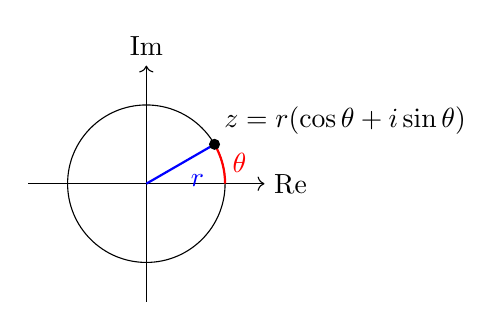
\begin{tikzpicture}
    % Axis
    \draw[->] (-1.5,0) -- (1.5,0) node[right] {$\text{Re}$};
    \draw[->] (0,-1.5) -- (0,1.5) node[above] {$\text{Im}$};

    % Unit circle
    \draw (0,0) circle [radius=1];

    % Complex number in polar form
    \coordinate (z) at (30:1);

    % Draw lines and angles
    \draw[blue, thick] (0,0) -- (z) node[midway, below right] {$r$};
    \draw[red, thick] (1,0) arc (0:30:1) node[midway, right] {$\theta$};

    % Draw complex number
    \fill (z) circle [radius=2pt] node[above right] {$z = r(\cos \theta + i \sin \theta)$};
\end{tikzpicture}
\end{figure}

$\\z_1 = (1,0) \rightarrow 1\\$
$z_2 = (1,\frac{\pi}{2}) \rightarrow i\\$
$z_3 = (1,\pi) \rightarrow -1\\$
$z_4 = (1,\frac{3\pi}{2}) \rightarrow -i\\$

\subsection{Forma trigonometrica di un numero complesso}

Dato un $z = (r, \alpha)$ in coordinate polari, vogliamo ricavare la forma algebrica.

\[\cos(\alpha) := \frac{a}{r} \hspace{20pt} \sin(\alpha) := \frac{b}{r}\]

\[z = r(\cos(\alpha)) + i\sin(\alpha)\]
è detta \textbf{forma trigonometrica di z.}
$\\$ $\\$ Esempio:

$\\\cos(0) + i\sin(0) = 1\\$
$\cos(\frac{\pi}{2}) + i\sin(\frac{\pi}{2}) = i\\$
$\cos(\pi) + i\sin(\pi) = -1\\$
$\cos(\frac{3\pi}{2}) + i\sin(\frac{3\pi}{2})) = -i\\$

In forma trigonometrica il prodotto diventa una somma di due angoli.

\subsubsection{Formula di De Moivre}

Dato $z = r(\cos(\alpha) + i\sin(\alpha) \in \mathbf{C}$ allora

\[z^n = r^n(\cos{(n \theta) + i\sin{(n \theta)}})\]

\subsection{Definizione}

$y \in \mathbf{C}, n \in \mathbf{N}$ si dicono radici n-esime di y le soluzioni dell'equazione $x^n = y$.

\subsection{Teorema}

Siano $y \in \mathbf{C}, n \in \mathbf{N}$ esistono precisamente n radici n-esime distinte $z_0, z_1, ... , z_{z-1}$ di y. Se:

\[y = r(\cos(\alpha) + i\sin(\alpha)\]
Allora:
\[z_0 = \sqrt{r}\left(\cos\left(\frac{\alpha}{n}\right) + i\sin\left(\frac{\alpha}{n}\right)\right)\]
\[z_k = \sqrt{r}\left(\cos\left(\frac{\alpha+(2\pi)k}{n}\right) + i\sin\left(\frac{\alpha+(2\pi)k}{n}\right)\right)\] per k = 1, ... $n-1$
$\\$ $\\$
Dimostrazione: Per la formula di de Moivre:

\[(z_k)^n = (\sqrt{r})^2(\cos(\alpha+(2\pi)k)) + i\sin(\alpha+(2\pi)k)\]

\begin{figure}[H]
\centering
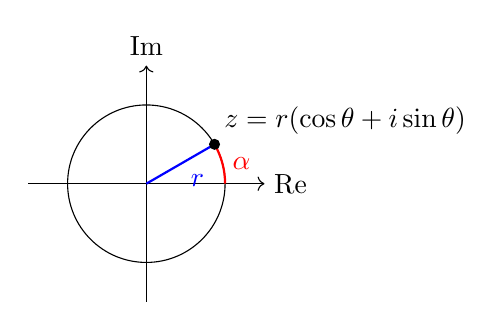
\begin{tikzpicture}
    % Axis
    \draw[->] (-1.5,0) -- (1.5,0) node[right] {$\text{Re}$};
    \draw[->] (0,-1.5) -- (0,1.5) node[above] {$\text{Im}$};

    % Unit circle
    \draw (0,0) circle [radius=1];

    % Complex number in polar form
    \coordinate (z) at (30:1);

    \draw[blue, thick] (0,0) -- (z) node[midway, below right] {$r$};
    \draw[red, thick] (1,0) arc (0:30:1) node[midway, right] {$\alpha$};

    % Draw complex number
    \fill (z) circle [radius=2pt] node[above right] {$z = r(\cos \theta + i \sin \theta)$};
\end{tikzpicture}
\end{figure}

\begin{figure}[H]
\centering
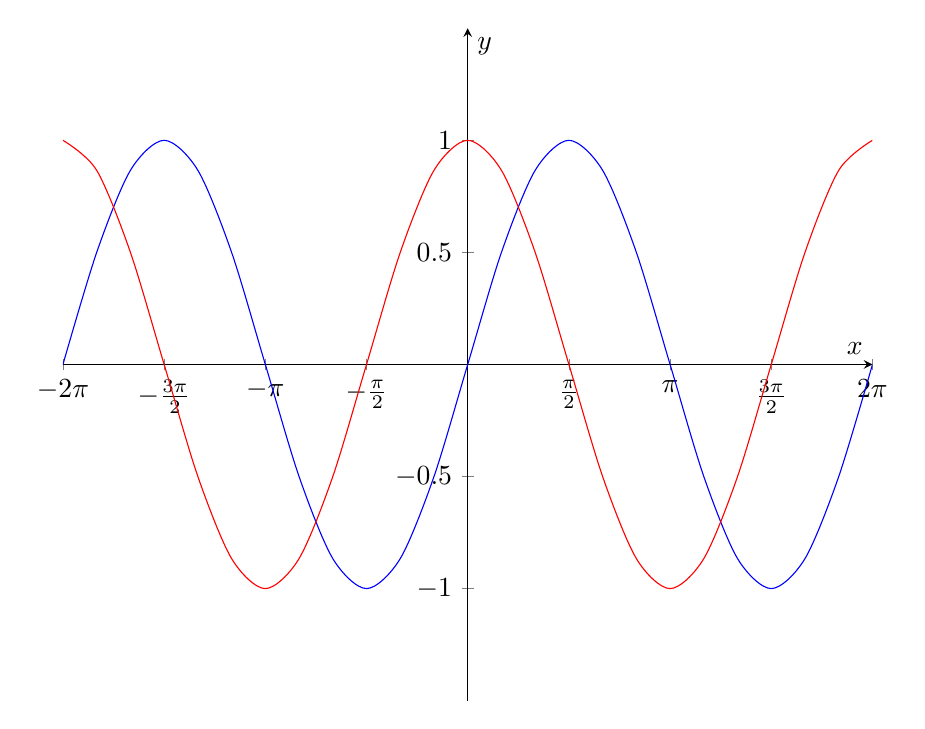
\begin{tikzpicture}
  \begin{axis}[
    scale=1.5,
    axis lines=middle,
    xlabel={$x$},
    ylabel={$y$},
    xmin=-2*pi, xmax=2*pi,
    ymin=-1.5, ymax=1.5,
    xtick={-2*pi, -3*pi/2, -pi, -pi/2, pi/2, pi, 3*pi/2, 2*pi},
    xticklabels={$-2\pi$, $-\frac{3\pi}{2}$, $-\pi$, $-\frac{\pi}{2}$, $\frac{\pi}{2}$, $\pi$, $\frac{3\pi}{2}$, $2\pi$},
    ytick={-1, -0.5, 0.5, 1},
    legend pos=outer north east,
  ]

  \addplot[domain=-2*pi:2*pi,smooth,variable=\x,blue] {sin(\x r)} node[right] {$\sin(x)$};
  \addplot[domain=-2*pi:2*pi,smooth,variable=\x,red] {cos(\x r)} node[right] {$\cos(x)$};

  \end{axis}
\end{tikzpicture}
\end{figure}

\[= r(\cos(\alpha) + i\sin(\alpha) = y\]
Quindi $z_0, ... z_{n-1}$ sono soluzioni di $y = x^n$, cioè sono radici n-esime di y. Siccome il periodo di sin e cos è $2\pi$, sono tutte distinte.

\subsection{Radici quadrate di numeri reali negativi}

Sia $a \in \mathbf{R} \subseteq \mathbf{C}$ tale che $a < 0$, esistono precisamente due radici quadrate di a in $\mathbf{C}$. Infatti, abbiamo:

\[a = (-a) (\cos(\pi) + i\sin(\pi)\]
Per Teorema 1.9:
\[z_0 = \sqrt{-a}\left(\cos\left(\frac{\pi}{2}\right) + i\sin\left(\frac{\pi}{2}\right)\right) = i\sqrt{-a}\]
\[z_1 = \sqrt{-a}\left(\cos\left(\frac{3\pi}{2}\right) + i\sin\left(\frac{3\pi}{2}\right)\right) = i\sqrt{-a}\]
NB: $ax^2 + bx + c, a, b, c \in \mathbf{R}$ o $\mathbf{C}$
Quindi: $\frac{-b+-\sqrt{b^2-4ac}}{2a}$ esistono due soluzioni anche se $\Delta < 0$.

\pagebreak

\section{Sistemi lineari e matrici}

\subsection{Sistemi lineari}

Esempio: valori nutrizionali (per porzione)

\begin{table}[H]
\centering
\begin{tabular}{|c|c|c|}
    \hline
    & Cheerios & Quakers\\
    \hline
    Proteine(g) & 4 & 3\\
    \hline
    Carbs (g) & 20 & 18\\
    \hline
    Grassi (g) & 2 & 5\\
    \hline
\end{tabular}
\end{table}
$\\$
Quanti porzioni di Quakers e Cheerios ci danno una colazione con 9 g di proteine, 48 g di carboidrati e 8g di grassi?

\begin{align*}
  \begin{cases}
    4c + 3q = 9\\
    20c + 18q = 48\\
    2c + 5q = 8
  \end{cases}
\end{align*}
Un sistema lineare è un insieme di m equazioni in n incognite, che può essere scritto nel modo seguente:

\[a_{11}x_1 + a_{12}x_2 + ... + a_{1n}x_n = b_1\]
\[...\]
\[a_{n1}x_1 + a_{n2}x_2 + ... + a_{nn}x_n = b_n\]
dove $b_k, a_ij \in \mathbf{C}$ oppure $\mathbf{R}$ per $1 <= i <= n, 1 <= j <= n, 1 <= k <= n$. Se i termini noti sono tutti nulli il sistema è detto omogeneo. $\\$
Una n-upla $(x_1, ... x_n)$ di numeri complessi (o reali) è una \textit{soluzione} se soddisfa tutte le n equazioni.
$\\$$\\$
Esempio: $\\$
4C + 3Q = 9 (I)\\
20C + 18Q = 48 (II)\\
2C + 5Q = 8 (III) \\
\\
Moltiplichiamo  (I) per $\frac{1}{4}$ e otteniamo un sistema lineare equivalente (cioè avendo \textit{esattamente} le stesse soluzioni).
\begin{center}
(I') C + $\frac{1}{4}$Q = $\frac{9}{4}$\\
(II) 20C + 18Q = 48\\
(III) 2C + 5Q = 8\\
\end{center}
Calcolando (II) - 20(I') e (III) - 2(I') si ottiene un altro sistema lineare equivalente.
\begin{center}
(I') C + $\frac{1}{4}$Q = $\frac{9}{4}$\\
(II') 0C + 3Q = 3\\
(III') 0C + $\frac{7}{2}$Q = $\frac{7}{2}$\\
\end{center}
Moltiplichiamo (II') per $\frac{1}{3}$ si ottiene
\begin{center}
(I') C + $\frac{1}{4}$Q = $\frac{9}{4}$\\
(II'')  + Q = 1\\
(III')  + $\frac{7}{2}$Q = $\frac{7}{2}$\\
\end{center}
Calcolando (III')-$\frac{7}{2}$(II') si ottiene:
\begin{center}
(I') C + $\frac{1}{4}$Q = $\frac{9}{4}$\\
(II'')  + Q = 1\\
(III')  + 0 = 0\\
\end{center}
Otteniamo dunque che Q = 1 e $C = \frac{9}{4} - \frac{3}{4} = \frac{7}{4}$.

$\\$
Analogamente possiamo risolvere il sistema lineare:

\[\begin{pmatrix}[cc|c]
  4 & 3 & 9\\
  20 & 18 & 48\\
  2 & 5 & 8
\end{pmatrix}\]

\[\rightarrow \frac{1}{4}\mathbf{R1}\]

\[\begin{pmatrix}[cc|c]
  1 & \frac{3}{4} & \frac{9}{4}\\
  20 & 18 & 48\\
  2 & 5 & 8
\end{pmatrix}\]

\[\rightarrow R2 - 20(R1), R3 - 2(R1)\]

\[\begin{pmatrix}[cc|c]
  1 & \frac{3}{4} & \frac{9}{4}\\
  0 & 3 & 3\\
  0 & \frac{7}{2} & \frac{7}{2}
\end{pmatrix}\]

\[\rightarrow \frac{1}{3}R3\]

\[\begin{pmatrix}[cc|c]
  1 & \frac{3}{4} & \frac{9}{4}\\
  0 & 1 & 1\\
  0 & \frac{7}{2} & \frac{7}{2}
\end{pmatrix}\]

\[\rightarrow R3 - \frac{7}{2}R2\]

\[\begin{pmatrix}[cc|c]
  1 & \frac{3}{4} & \frac{9}{4}\\
  0 & 1 & 1\\
  0 & 0 & 0
\end{pmatrix}\]

\subsection{Definizione}
Siano $n, n \ge 1$ una tabella

\begin{center}
A =
$\begin{pmatrix}
a_{11} & ... & a_{1n}\\
a_{n1} & ... & a_{nn}
\end{pmatrix}$ = $(a_{ij})$
\end{center}
di nxn elementi di $\mathbf{C}$ disposti in n righe e n colonne si chiama matrice di dimensione nxn. Gli elementi si dicono \textit{coefficenti} (o \textit{entrate}) della matrice e sono contrassegnati con un doppio indice ij dove i indica la rigaa e la j indica la colonna di appartenenza.\\
$M_{nxn}(\mathbf{C})$ = L'insieme di tutte le matrici di dimensioni nxn con entrate $\mathbf{C}$\\
$M_{nxn}(\mathbf{R})$ = L'insieme di tutte le matrici di dimensioni nxn con entrate $\mathbf{R}$\\
\\
ESEMPIO:

\begin{center}
$\begin{pmatrix}
3 & i & 2+7i\\
0 & 1 & \pi
\end{pmatrix} \in M_{2x3} (\mathbf{C})$
\end{center}

\begin{center}
$\begin{pmatrix}
0 & 1\\
1 & -1
\end{pmatrix} \in M_{2x2} (\mathbf{R}) \subseteq M_{2x2} (\mathbf{C})$
\end{center}

\subsection{Definizione: forma matriciale}

Un sistema lineare di n incognite e n equazioni:

\[a_{11}x_1 + a_{12}x_2 + ... + a_{1n}x_n = b_1\]
\[...\]
\[a_{n1}x_1 + a_{n2}x_2 + ... + a_{nn}x_n = b_n\]
$\\$
può essere rappresentato nella forma matriciale:

\[Ax = b\]
\begin{figure}[H]
\centering
A =
$\begin{pmatrix}
a_{11} & ... & a_{1n}\\
a_{n1} & ... & a_{nn}
\end{pmatrix}$
\end{figure}

\begin{center}
x =
$\begin{pmatrix}
x_1\\
...\\
x_n
\end{pmatrix}$
\end{center}

\begin{center}
b =
$\begin{pmatrix}
b_1\\
...\\
b_n
\end{pmatrix}$ vettore dei termini noti
\end{center}

\begin{center}
La matrice
$\begin{pmatrix}[c|c]
A & B
\end{pmatrix} =
\begin{pmatrix}[ccc|c]
a_{11} & ... & a_{1n} & b_1\\
a_{n1} & ... & a_{nn} & b_n
\end{pmatrix}
$
\end{center}
è detta \textbf{matrice aumentata.}
\\\\
Esempio:
\begin{align*}
  \begin{cases}
    2x_1 + 6x_2 + 3x_3 + 2x_4 = 4\\
    x_1 - 2x_2 + \frac{1}{2}x_3 + \frac{9}{4}x_4 = 1\\
    -x_1 + x_2 - \frac{1}{2}x_3 - x_4 = \frac{2}{5}
  \end{cases}
\end{align*}

\[\begin{pmatrix}[cccc|c]
  2 & 6 & 3 & 2 & 4\\
  1 & -2 & \frac{1}{2} & \frac{9}{2} & 1 \\
  -1 & 1 & -\frac{1}{2} & -1 & \frac{2}{5}
\end{pmatrix}\]

\[\sim \frac{1}{2}R1\]

\begin{center}
$R2 - R1, R3 + R1 \sim
\begin{pmatrix}[cccc|c]
  1 & 3 & \frac{3}{2} & 1 & 2\\
  1 & -2 & \frac{1}{2} & \frac{9}{2} & 1 \\
  -1 & 1 & -\frac{1}{2} & -1 & \frac{2}{5}
\end{pmatrix}$
\end{center}

\begin{center}
$-\frac{1}{5}R2 \sim
\begin{pmatrix}[cccc|c]
  1 & 3 & \frac{3}{2} & 1 & 2\\
  0 & -5 & -1 & \frac{5}{4} & -1 \\
  0 & 4 & 1 & 0 & \frac{12}{5}
\end{pmatrix}$
\end{center}

\begin{center}
$ R3 - 4R2 \sim
\begin{pmatrix}[cccc|c]
  1 & 3 & \frac{3}{2} & 1 & 2\\
  0 & 1 & \frac{1}{5} & -\frac{1}{4} & \frac{1}{5} \\
  0 & 0 & \frac{1}{5} & 1 & \frac{8}{5}
\end{pmatrix}$
\end{center}

\begin{center}
$5R3 \sim
\begin{pmatrix}[cccc|c]
  1 & 3 & \frac{3}{2} & 1 & 2\\
  0 & 1 & \frac{1}{5} & -\frac{1}{4} & \frac{1}{5} \\
  0 & 0 & 1 & 5 & 8
\end{pmatrix}$
\end{center}
Si ottiene il sistema lineare:
\begin{align*}
  \begin{cases}
    x_1 + 3x_2 + \frac{3}{2}x_3 + x_4 = 2\\
    2x_2 + \frac{1}{5}x_3 - \frac{1}{4}x_4 = \frac{1}{5}\\
    x_3 + 5x_4 = 8
  \end{cases}
\end{align*}
Assegniamo un parametro alla variabile libera $x_4$: $t = x_4$. Possiamo scrivere la soluzione con un parametro.

\[x_4 = t\]
\[x_3 = 8 - 5t\]
\[x_2 = \frac{1}{5} - \frac{1}{5}(8-5t) + \frac{1}{4}t\\= -\frac{7}{5} + t - \frac{1}{4}t = -\frac{7}{5} + \frac{5}{4}t\]
\[x_1 = 2 - 3(-\frac{7}{5}+\frac{5}{4}t) - \frac{3}{2}(8-5t) - 5\\=2 + \frac{21}{5} - 12 - \frac{15}{4}t + \frac{15}{2}t - t=\]
\[\frac{10+21-60}{5} - \frac{15+30}{4}t - t = -\frac{29}{5} + \frac{15}{4}t - \frac{4}{4}t = -\frac{29}{5} + \frac{11}{4}t\]
Il sistema ha infinite soluzioni, una per ogni t $\in \mathbf{C}$.

\subsection{Operazioni elementari}

Attraverso le seguenti operazioni sulla matrice aumentata (A | b), si ottiene un sistema equivalente più semplice:

\begin{itemize}
    \item Moltiplicare riga i (Ri) per uno scalare ($\alpha \in \mathbf{C})$. Questa operazioni non cambia le soluzioni del sistema se lo scalare non è $\neq 0$.
    \item Sommare una riga (Ri) con un multiplo di un'altra riga(Rj): Ri + $\alpha$Rj
    \item Scambiare riga i (Ri) e riga j (Rj): $R_i \longleftrightarrow R_j$
\end{itemize}
Esempio:
\begin{align*}
  \begin{cases}
    2x_1 + 6x_2 + 3x_3 = 4\\
    x_1 - 2x_2 - \frac{1}{2}x_3 = 1\\
    -x_1 + x_2 - \frac{7}{10} = \frac{2}{5}
  \end{cases}
\end{align*}
Applichiamo l'algoritmo \textit{Eliminazione di Gauss}.
\begin{center}
$\begin{pmatrix}[ccc|c]
  2 & 6 & 3 & 4\\
  1 & -2 & \frac{1}{2} & 1\\
  -1 & 1 & \frac{7}{10} & \frac{2}{5}
\end{pmatrix}$
\end{center}

\begin{center}
$\sim \frac{1}{2}$R1
$\begin{pmatrix}[ccc|c]
  1 & 3 & \frac{3}{2} & 2\\
  1 & -2 & \frac{1}{2} & 1\\
  -1 & 1 & \frac{7}{10} & \frac{2}{5}
\end{pmatrix}$
\end{center}

\begin{center}
$\sim $R2 - R1, R3 + R1
$\begin{pmatrix}[ccc|c]
  1 & 3 & \frac{3}{2} & 2\\
  0 & -5 & -1 & -1\\
  0 & 4 & \frac{4}{5} & \frac{12}{5}
\end{pmatrix}$
\end{center}

\begin{center}
$\sim -\frac{1}{5}$R2
$\begin{pmatrix}[ccc|c]
  1 & 3 & \frac{3}{2} & 2\\
  0 & 1 & \frac{1}{5} & \frac{1}{5}\\
  0 & 4 & \frac{4}{5} & \frac{12}{5}
\end{pmatrix}$
\end{center}

\begin{center}
$\sim$R3 - 4R2
$\begin{pmatrix}[ccc|c]
  1 & 3 & \frac{3}{2} & 2\\
  0 & 1 & \frac{1}{5} & \frac{1}{5}\\
  0 & 0 & 0 & \frac{8}{5}
\end{pmatrix}$
\end{center}
Lo scopo dell'algoritimo è di avere degli 1 in "diagonale" nella matrice.
\begin{center}
$\sim \frac{5}{8}$R3
$\begin{pmatrix}[ccc|c]
  1 & 3 & \frac{3}{2} & 2\\
  0 & 1 & \frac{1}{5} & \frac{1}{5}\\
  0 & 0 & 0 & 1
\end{pmatrix}$
\end{center}
Otteniamo un sistema lineare equivalente:
\[x_1 + 3x_2 + \frac{3}{2}x_3 = 2\]
\[x_2 + \frac{1}{5}x_3 = \frac{1}{5}\]
\[0 = 1\]
0 non è mai uguale uno e quindi non esistono soluzioni a questo sistema lineare.

\subsection{Linee in $\mathbf{R^2}$}

Consideriamo 2 equazioni in 2 incognite con coefficienti $\in \mathbf{R}$:
\begin{align*}
  \begin{cases}
    a_{11}x + a_{12}y = b_1\\
    a_{21}x + a{22}y = b_2
  \end{cases}
\end{align*}

dove $a_{11}, a_{12}, a_{21}, a{22} \in \mathbf{R}$

\[\rightarrow y = -\frac{a_{11}}{a_{12}}x + \frac{b_1}{a_{12}} (I)\]
\[y = -\frac{a_{21}}{a_{22}}x + \frac{b_2}{a_{22}} (II)\]

1. Soluzione dove le due rette sul piano cartesiano si incontrano.

\begin{figure}[H]
  \centering
  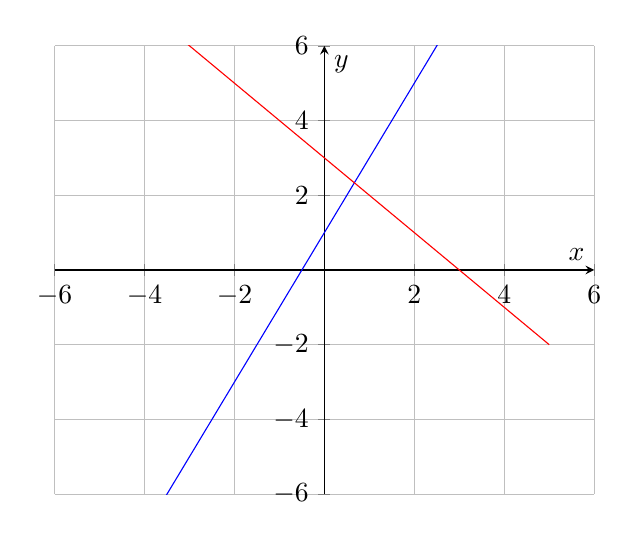
\begin{tikzpicture}
    \begin{axis}[
      xlabel=$x$,
      ylabel=$y$,
      grid=major,
      axis lines=middle,
      enlargelimits = true,
      ymin=-5, ymax=5,
      xmin=-5, xmax=5,
    ]

    % Line 1: y = 2x + 1
    \addplot[blue, domain=-5:5, samples=100] {2*x + 1};
    % Line 2: y = -x + 3
    \addplot[red, domain=-5:5, samples=100] {-x + 3};

    \end{axis}
  \end{tikzpicture}
  \caption{Rette incidenti: 1 soluzioni}
\end{figure}
2. Soluzione dove le due linee sono parallele (0 soluzioni)
\begin{figure}[H]
  \centering
  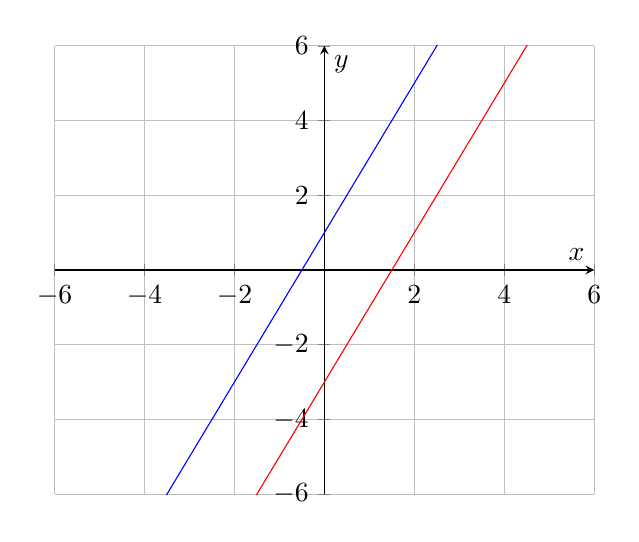
\begin{tikzpicture}
    \begin{axis}[
      xlabel=$x$,
      ylabel=$y$,
      grid=major,
      axis lines=middle,
      enlargelimits = true,
      ymin=-5, ymax=5,
      xmin=-5, xmax=5,
    ]

    % Line 1: y = 2x + 1
    \addplot[blue, domain=-5:5, samples=100] {2*x + 1};
    % Line 2: y = -x + 3
    \addplot[red, domain=-5:5, samples=100] {2*x-3};

    \end{axis}
  \end{tikzpicture}
  \caption{Rette parallele: 0 soluzioni}
\end{figure}
3. Infinite soluzioni
\begin{figure}[H]
  \centering
  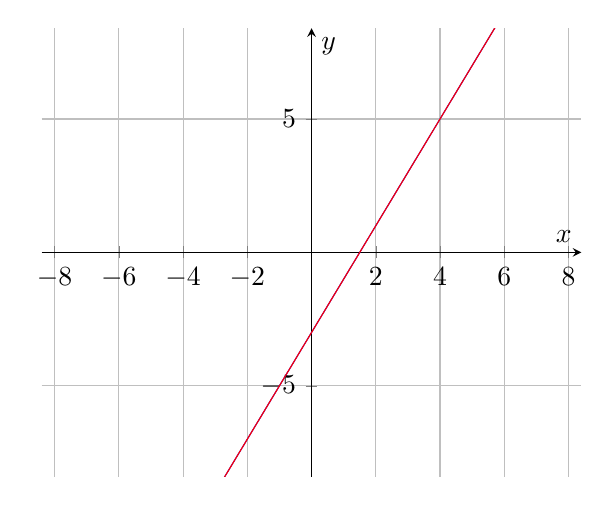
\begin{tikzpicture}
    \begin{axis}[
      xlabel=$x$,
      ylabel=$y$,
      grid=major,
      axis lines=middle,
      enlargelimits = true,
      ymin=-7, ymax=7,
      xmin=-7, xmax=7,
    ]

    % Line 1: y = 2x + 1
    \addplot[blue, domain=-7:7, samples=100] {2*x - 3};

    % Line 2: y = -x + 3
    \addplot[red, domain=-7:7, samples=100] {2*x-3};

    \end{axis}
  \end{tikzpicture}
  \caption{Rette coincidenti: $\infty$ soluzioni}
\end{figure}

\subsection{Metodo di eliminazione di Gauss (EG)}
Data una matrice M = ($a_{ij}$) in $M_{nxn} (\mathbf{C})$ (oppure in $M_{nxn} (\mathbf{R}$) con righe R1, ... Rn, eseguiamo le seguenti operazioni elementari:

\begin{itemize}
    \item Scegliamo la prima colonna non nulla j di M (partendo da sinistra). Dopo aver eventualmente scambiato due righe di M, otteniamo una matrice della forma:
    \[\begin{pmatrix}
        0 & ... & 0 & a_{ij} & ... & a_{in}\\
        . & . & . & . & . & .\\
        . & . & . & . & . & .\\
        . & . & . & . & . & .\\
        0 & ... & 0 & a_{nj} & ... & a_{nn}
    \end{pmatrix}\]
    Moltiplicando R1 per $\frac{1}{a_{ij}}$, si ottiene
    \[\begin{pmatrix}
        0 & ... & 0 & 1 & * & ... & a_{in}\\
        . & . & . & . & . & .\\
        . & . & . & . & . & .\\
        . & . & . & . & . & .\\
        0 & ... & 0 & a_{nj} & a_{nj+1} & ... & a_{nn}
    \end{pmatrix}\]
    Adesso per ogni $2 \le i \le n$, eseguiamo l'operazione elementare Ri - $a_{ij}$R1. Otteniamo una matrice di forma:
    \[\begin{pmatrix}
        0 & ... & 0 & 1 & * & ... & * \\
        . & . & . & . & . & .\\
        . & . & . & . & . & .\\
        . & . & . & . & . & .\\
        0 & ... & 0 & 0 & * & ... & *
    \end{pmatrix}\]
    \item Ripetiamo il procedimento (a) sia M' per ottenere:
    \[\begin{pmatrix}
        0 & ... & 0 & 1 & * & ... & ... & *\\
        0 & ... & 0 & 0 & 1 & 0 & * & *\\
        0 & ... & 0 & 0 & 0 & 0 &  & *
    \end{pmatrix}\]
    \item Dopo un numero finito di passi , si ottiene una matrice che è una matrice a scala

    //Rifare matrice

    cioè esiste un numero $1 \le r \le n$ tale che:
    \begin{enumerate}
        \item Le righe $1 \le i \le r$ sono non nulle
        \item Ogni riga $2 \le i \le n$ ha un numero di zeri iniziali superiore alla riga precedente
        \item Le righe $r+1 \le i \le n$ sono tutte nulle.
    \end{enumerate}
    Inoltre il primo coefficiente non nullo di ogni riga è uguale a 1 ed è detto \textit{pivot}. La matrice è detta \textit{forma ridotta} di M. Le colonne che contengono un pivot vengono chiamate \textit{dominanti}.
\end{itemize}
Esempio:

\begin{center}
M =
$\begin{pmatrix}
  0 & 0 & 0 & 5 & 4\\
  0 & 10 & 0 & 30 & 2\\
  0 & -i & 0 & 6 & 7
\end{pmatrix} \in M_{3x5} \in \mathbf{C}$
\end{center}

\begin{center}
$R1 \longleftrightarrow R2$
$\begin{pmatrix}
  0 & 10 & 0 & 30 & 2\\
  0 & 0 & 0 & 5 & 4\\
  0 & -i & 0 & 6 & 7
\end{pmatrix}$
\end{center}

\begin{center}
$\frac{1}{10}R1$
$\begin{pmatrix}
  0 & 1 & 0 & 3 & \frac{1}{5}\\
  0 & 0 & 0 & 5 & 4\\
  0 & -i & 0 & 6 & 7
\end{pmatrix}$
\end{center}

\begin{center}
$R3 + iR1$
$\begin{pmatrix}
  0 & 1 & 0 & 3 & \frac{1}{5}\\
  0 & 0 & 0 & 5 & 4\\
  0 & 0 & 0 & 6+3i & 7+\frac{1}{3}i
\end{pmatrix}$
\end{center}

\begin{center}
$\frac{1}{5}R2$
$\begin{pmatrix}
  0 & 1 & 0 & 3 & \frac{1}{5}\\
  0 & 0 & 0 & 1 & \frac{4}{5}\\
  0 & 0 & 0 & 6+3i & 7+\frac{1}{3}i
\end{pmatrix}$
\end{center}

\begin{center}
$R3 - (6+3i)R2$
$\begin{pmatrix}
  0 & 1 & 0 & 3 & \frac{1}{5}\\
  0 & 0 & 0 & 1 & \frac{4}{5}\\
  0 & 0 & 0 & 0 & \frac{11}{5} - \frac{11}{5}i
\end{pmatrix}$
\end{center}

\[(7+\frac{1}{5}i - (6+3i)\frac{4}{5} = (7+\frac{1}{5}i) - \frac{24}{5} + \frac{12}{5}i = \frac{11}{5} - \frac{11}{5}i\]

\begin{center}
$\frac{1}{\frac{11}{5} - \frac{11}{5}i}R3$
$\begin{pmatrix}
  0 & 1 & 0 & 3 & \frac{1}{5}\\
  0 & 0 & 0 & 1 & \frac{4}{5}\\
  0 & 0 & 0 & 0 & 1
\end{pmatrix}$
\end{center}

\subsection{Risoluzione di sistema lineare}

Dato un sistema lineare

\[(*)  Ax = b\]
con A $\in M_{nxn} (\mathbf{C}), b \in M_{nx1} (\mathbf{C})$ procediamo con (EG) sulla matrice aumentata $(A | b)$ fino ad ottenere la forma ridotta $(u | c)$ e sistema lineare corrispondente:
\[ux = c\]
che è equivalente a (*). Chiamiamo \textbf{variabili dominanti} le r variabilic he corrispondono alle colonne dominanti e \textbf{variabili libere} le rimanenti:

Esempio:

\begin{align*}
  \begin{cases}
    10x_1 + 10x_2 + 30x_3 = 2\\
    5x_3 = 4\\
    -x_1 - x_2 + 6x_3 = 7
  \end{cases}
\end{align*}

\begin{center}
$\begin{pmatrix}[ccc|c]
  10 & 10 & 30 & 2\\
  0 & 0 & 5 & 4\\
  -1 & -1 & 6 & 7
\end{pmatrix}$
\end{center}

\begin{center}
$(EG) \Rightarrow$
$\begin{pmatrix}[ccc|c]
  1 & 1 & 3 & \frac{1}{4}\\
  0 & 0 & 1 & \frac{4}{5}\\
  0 & 0 & 0 & 0\\
  x_1 & x_2 & x_3
\end{pmatrix}$
\end{center}
$x_1$ e $x_3$ sono variabili dominanti e $x_2$ è variabile libera.\\
Si ha uno dei seguenti casi:\\
$[1]:$ Tutte le colonne di $(u | c)$ tranne c sono dominanti. In tal caso, il sistema ammette una e una sola soluzione.
\\
Esempio 2.1:
\begin{center}
$\begin{pmatrix}[cc|c]
  1 & \frac{3}{4} & \frac{9}{4}\\
  0 & 1 & 1\\
  0 & 0 & 0
\end{pmatrix}$
\end{center}
$[\infty]:$ L'ultima colonna e almeno colonna di u \textit{non} sono dominanti. In tal caso un sistema ammette infinite soluzioni che possiamo ottenere assegnando parametri per ogni colonna libera.
\\
Esempio 2.3:
\begin{center}
$\begin{pmatrix}[cccc|c]
  1 & 3 & \frac{3}{2} & 1 & 2\\
  0 & 1 & \frac{1}{5} & -\frac{1}{4} &  \frac{1}{5}\\
  0 & 0 & 1 & 5 & 8
\end{pmatrix}$
\end{center}
$[0]:$ L'ultima colonna c è dominante in tal caso il sistema non ammette soluzione.
\\
Esempio 2.4:

\begin{center}
$\begin{pmatrix}[ccc|c]
  1 & 3 & \frac{3}{2} & 2\\
  0 & 1 & \frac{1}{5} & \frac{1}{5}\\
  0 & 0 & 0 & 1
\end{pmatrix}$
\end{center}
Attenzione: La forma ridotta di una matrice \textbf{non è unica} ma le colonne dominanti sono univocamente determinate.

\subsection{Definizione}

Sia $A \in M_{nxn} (\mathbf{C}))$ con forma ridotta U. Il numero r di righe non nulle, pari al numero di colonne dominanti, è detto \textbf{rango} di u e si indica rku (rank). Dimostreremo più avanti che ogni forma ridotta di A ha lo stesso rango, quindi definiamo il rango di A come rkA (rango di A) = rkU (rango di U).
\\
Si ha $rkA \le min(n,n)$

\subsection{Osservazione}

Possiamo ricavare le condizioni $[1], [\infty], [0]$  usando il rango:

\subsubsection{Teorema di Rouchè-Capelli}

Sia $A \in M_{nxn} (\mathbf{C}),$ sia $b \in M_{nxi} (\mathbf{C})$.

\[[1] \Longleftrightarrow rkA = rk(A | b) = n\]
\[rkU = rk(u | c)\]
\[[\infty] \Longleftrightarrow rkA = rk(A | b) < n\]
\[[0] \Longleftrightarrow rkA < rk(A | b)\]

\pagebreak

\section{Matrici e le loro operazioni}

\subsection{Definizione}
Sia $A = (a_{ij})_{1 \le i \le n, 1 \le j \le n}$ e $B = (b_{ij})_{1 \le i \le n, 1 \le j \le n}$ matrici in $M_{nxn} \mathbf{C}$.
Diciamo \textbf{somma} di A e B la matrice:
\[A + B = (a_{ij} + b_{ij})\]
\[= a_{11} + b{11} \dots a_{1n} + b_{1n}\]
\[= a_{21} + b{21} \dots a_{2n} + b_{2n}\]
\[= a_{n1} + b{n1} \dots a_{nn} + b_{nn}\]
in $M_{nxn}\mathbf{C}$.
\\
Esempio:

\begin{center}
$\begin{pmatrix}
  1 & 0 & i\\
  3 & 1 & 4
\end{pmatrix} +$
$\begin{pmatrix}
    2 & 4 & 1\\
    2 & -i & 1+i
\end{pmatrix} =$
$\begin{pmatrix}
    3 & 4 & 1+i\\
    -1 & 1-i & 5+i
\end{pmatrix}$
\end{center}
\textbf{Proprietà}: L'addizione di matrice è associativa (cioè (A+B)+C = A+(B+C)) e commutativa (cioè A+B = B+A)

\subsection{Definizione}

Data una matrice  $A = (a_{ij})_{1 \le i \le n, 1 \le j \le n} \in M_{nxn} \mathbf{C}$ e $\alpha \in \mathbf{C}$, diciamo prodotto della matrice A per lo scalare $\alpha$ la matrice:
\[
\alpha A = (\alpha a_{ij}) \in M_{nxn} (\mathbf{C})
\]

\begin{center}
$\frac{1}{2}$
$\begin{pmatrix}
  2+i & 5\\
  i & 1-2i
\end{pmatrix} =$
$\begin{pmatrix}
    1+\frac{1}{2}i & \frac{5}{2}\\
    \frac{1}{2}i & \frac{1}{2} - i
\end{pmatrix}$
\end{center}
\textbf{Proprietà}:

\[\alpha(A+B) = \alpha A + \alpha B\\(\alpha + \beta)A = \alpha A + \beta A.\]
\\per $A, B \in M_{nxn} (\mathbf{C}), \alpha, \beta \in \mathbf{C}.$

\subsection{Definizione}

Accanto a una matrice $A = (a_{ij}) \in M_{nxn} (\mathbf{C})$, consideriamo la matrice $A^t$ ottenuta da A scambiando le righe per le colonne detta trasposta di A.
\\
Esempio:

\begin{center}
$A =$
$\begin{pmatrix}
  1 & i & 7\\
  \pi & \frac{1}{12} & 0
\end{pmatrix} A^t = $
$\begin{pmatrix}
    1 & \pi\\
    i & \frac{1}{12}\\
    7 & 0
\end{pmatrix}$
\end{center}

\subsection{Prodotto di matrici}

(a) Una matrice di dimensione nx1 è detta vettore (colonna) e si usa la notazione:

\[v = \begin{pmatrix}
    v_1\\
    .\\
    .\\
    .\\
    v_n
\end{pmatrix} \in M_{nx1} (\mathbf{C})\]
Una matrice di dimensione 1xn è detta vettore riga e si usa la notazione $v^t$.

\[v^t = \begin{pmatrix}
    v_1 & \dots & v_n
\end{pmatrix} \in M_{1xn} (\mathbf{C})\]
Siano $v^t$ un vettore riga in $M_{1xn} (\mathbf{C})$ e u un vettore colonna in $M_{nx1} (\mathbf{C})$. Si chiama \textbf{prodotto di $v^t$ con u} il numero complesso $v^t_u = v_1u_1 + v_2u_2 + ... + v_nu_n \in \mathbf{C}$.
\\\\
Esempio:

\begin{center}
$v^t =$
$\begin{pmatrix}
  1 & 2 & 3
\end{pmatrix} u = $
$\begin{pmatrix}
    1\\
    0\\
    3
\end{pmatrix}$
\end{center}
\[v^t_u = 1 + 0 + 9 = 10.\]
\\
(b) possiamo vedere una matrice $A = (a_{ij})$ come n vettori riga $R_i = (a_{i1}...a_{in})$ detti \textbf{righe di A} oppure n vettori colonna: $c_j = \begin{pmatrix}
    a_{ij}\\
    .\\
    .\\
    .\\
    a_{nj}
\end{pmatrix}$ detti \textbf{colonne di A}.
\\
Esempio:
\[
A =
\begin{pmatrix}
    10 & 2 & 1\\
    2i & 4 & 0\\
    0 & 2 & 8
\end{pmatrix} =
\begin{pmatrix}
    10 & 2 & 1\\
    2i & 4 & 0\\
    0 & 2 & 8
\end{pmatrix}
\]
Siano $A = (a_{ij}) \in M_{nxn} \in \mathbf{C}$ e $B = (b_{ij}) \in M_{nxn} \in \mathbf{C}$ se n = s, allora possiamo formare il prodotto di A e B:

\[AB = (c_{ij})\]
dove $c_{ij} = R_iC_j =
$
$\begin{pmatrix}
  a_{i1} & \dots & a_{in}
\end{pmatrix}$
$\begin{pmatrix}
    b_{ij}\\
    .\\
    .\\
    .\\
    b_{nj}
\end{pmatrix}$
è il prodotto della riga i di A e la colonna j di B.
\\\\
Esempio:

\begin{center}
$v^t =$
$\begin{pmatrix}
  1 & 2 & 3\\
  0 & 1 & 4
\end{pmatrix} \cdot$
$\begin{pmatrix}
    1 & 4 & 0\\
    0 & 1 & 5\\
    1 & 2 & 4
\end{pmatrix} = $
$\begin{pmatrix}
    R1C1 & R1C2 & R1C3\\
    R2C1 & R2C2 & R2C3
\end{pmatrix} = $
$\begin{pmatrix}
    4 & 12 & 22\\
    4 & 9 & 21
\end{pmatrix}$
\end{center}
\textbf{Proprietà}:

\begin{itemize}
    \item Il prodotto di matrici è associativo: \[(AB)C = A(BC)\]
    \item Leggi distributive: \[(A+B)C = AC + BC\]
    \[A(B+C) = AB + AC\]
    \item Scriviamo $I_n \in M_{nxn} (\mathbf{C})$ per la matrice ridotta e diciamo \textbf{matrice identità}.

ESEMPIO:

\begin{center}
$I_3 =$
$\begin{pmatrix}
  1 & 0 & 0\\
  0 & 1 & 0\\
  0 & 0 & 1
\end{pmatrix} I_2 = $
$\begin{pmatrix}
  1 & 0\\
  0 & 1
\end{pmatrix} M = $
$\begin{pmatrix}
  1 & 2\\
  3 & 4
\end{pmatrix}$\\
$MI_2 = \begin{pmatrix}
  1 & 2\\
  3 & 4
\end{pmatrix}$
$\begin{pmatrix}
  1 & 0\\
  0 & 1
\end{pmatrix} = $
$\begin{pmatrix}
    1 & 2\\
    3 & 4
\end{pmatrix} = M$
\end{center}
Per ogni matrice $M = \in M_{nxn} (\mathbf{C})$ abbiamo che $MI_n = M = I_nM$

\item $(AB)^t = B^tA^t$\\\\
ESEMPIO:
\begin{center}
    $A = \begin{pmatrix}
        1 & 0\\
        2 & 1
    \end{pmatrix} \cdot B = $
    $\begin{pmatrix}
        1 & 2 & 4\\
        0 & 1 & 5
    \end{pmatrix} = $
    $\begin{pmatrix}
        1 & 2 & 4\\
        2 & 5 & 13
    \end{pmatrix}$
\end{center}
\begin{center}
    $A^t = \begin{pmatrix}
        1 & 2\\
        0 & 1
    \end{pmatrix} \cdot B^t = $
    $\begin{pmatrix}
        1 & 0\\
        2 & 1\\
        4 & 5
    \end{pmatrix} = $
    $\begin{pmatrix}
        1 & 2\\
        2 & 5\\
        4 & 13
    \end{pmatrix} = (AB)^t$
\end{center}

\begin{center}
    $B^tA^t = \begin{pmatrix}
        1 & 0\\
        2 & 1\\
        4 & 5
    \end{pmatrix}$
    $\begin{pmatrix}
        1 & 2\\
        0 & 1
    \end{pmatrix} = $
    $\begin{pmatrix}
        1 & 2\\
        2 & 5\\
        4 & 13
    \end{pmatrix}$
\end{center}

\item Il prodotto tra matrici NON è commutativo.
\[AB \neq BA\]
\end{itemize}
\subsection{Osservazione}

Siano A = ($a_{ij}) \in M_{nxn} (\mathbf{C}$ e $b = \begin{pmatrix}
    b_1\\
    \vdots\\
    b_n
\end{pmatrix} \in M_{nx1} (\mathbf{C}), x = \begin{pmatrix}
    x_1\\
    \vdots\\
    x_n
\end{pmatrix}$. Consideriamo  Ax = b in forma matriciale. Abbiamo:

\begin{center}
$Ax = \begin{pmatrix}
    a_{11} & ... & a_{1n}\\
    \vdots & & \vdots\\
    a_{n1} & ... & a_{nn}
\end{pmatrix}\begin{pmatrix}
    x_1\\
    \vdots\\
    x_n
\end{pmatrix} = \begin{pmatrix}
    a_{11}x_1 + & ... & + a_{1n}x_n\\
    \vdots & & \vdots\\
    a_{n1}x_1 + & ... & + a_{nn}x_n
\end{pmatrix}$
\end{center}
è uguale a $b = \begin{pmatrix}
    b_1\\
    \vdots\\
    b_n
\end{pmatrix}$;

\begin{center}
    $\begin{pmatrix}
        b_1\\
        \vdots\\
        b_n
    \end{pmatrix} =
    \begin{pmatrix}
        a_{11}x_1 + & ... & + a_{1n}x_n\\
        \vdots & & \vdots\\
        a_{n1}x_1 + & ... & + a_{nn}x_n
    \end{pmatrix} \leadsto \begin{cases}
            a_{11}x_1 + ... + a_{1n}x_n = b_1\\
            \vdots\\
            a_{n1}x_1 + ... + a_{nn}x_n = b_n
        \end{cases}$
\end{center}
ESEMPIO:
\begin{center}
    $\begin{cases}
        2x_1 + 6x_2 = 4\\
        x_1 - 2x_2 = 1\\
        -x_1 + x_2 = \frac{2}{5}
    \end{cases}$
\end{center}

\begin{center}
    $A = \begin{pmatrix}
        2 & 6\\
        1 & -2\\
        -1 & 1
    \end{pmatrix} x = \begin{pmatrix}
        x_1\\
        x_2
    \end{pmatrix} b = \begin{pmatrix}
        4\\
        1\\
        \frac{2}{5}
    \end{pmatrix}$
\end{center}

\begin{center}
$Ax = \begin{pmatrix}
        2 & 6\\
        1 & -2\\
        -1 & 1
    \end{pmatrix}\begin{pmatrix}
        x_1\\
        x_2
    \end{pmatrix} = \begin{pmatrix}
        2x_1 & 6x_2\\
        x_1 & -2x_2\\
        -x_1 & x_2
    \end{pmatrix} = \begin{pmatrix}
        4\\
        1\\
        \frac{2}{5}
    \end{pmatrix}$
\end{center}

\subsection{Definizione}

Una matrice A = $a_{ij}$ di dimensione nxn si dice matrice quadrata di ordine n. Gli elementi di A $a_{ii}$ formano la \textbf{diagonale} di A.
\\\\
Esempio:

\[\begin{pmatrix}
    0 & -10 & i\\
    7 & 8 & 0\\
    100 & \frac{1}{2} & i
\end{pmatrix}\]
Se tutti gli elementi fuori dalla diagonale sono nulli, allora è detta \textbf{matrice diagonale}.
\\
Esempio:
\[\begin{pmatrix}
    0 & 0 & 0\\
    0 & 8 & 0\\
    0 & 0 & i
\end{pmatrix}\]
Se tutti i coefficienti al di sotto della diagonale sono nulli, allora la matrice è detta matrice \textbf{triangolare} superiore o inferiore.

\begin{center}
    $\begin{pmatrix}
        0 & -10 & i\\
        0 & 8 & 0\\
        0 & 0 & i
    \end{pmatrix} oppure \begin{pmatrix}
        0 & 0 & 0\\
        7 & 8 & 0\\
        100 & \frac{1}{2} & i
    \end{pmatrix} $
\end{center}

\subsection{Matrici elementari}

Prendiamo la matrice identità:

\[I_n = \begin{pmatrix}
    1 & 0 & ... & 0\\
    0 & 1 & ... & 0\\
    \vdots & \vdots & \ddots & \vdots\\
    0 & 0 & ... & 1
\end{pmatrix}\]
Applichiamo le operazioni elementari alla matrice identità $I_n$ per ottenere matrici elementari che denotiamo come segue:

\begin{itemize}

\item $E_{ij}$ la matrice ottenuta da $I_n$ scambiando la riga i con la riga j.
\\Esempio:
\[I_3 = \begin{pmatrix}
    1 & 0 & 0\\
    0 & 1 & 0\\
    0 & 0 & 1
\end{pmatrix}\]
\[E_{12} = \begin{pmatrix}
    0 & 1 & 0\\
    1 & 0 & 0\\
    0 & 0 & 1
\end{pmatrix}\]

\item $E_{i}(K)$ ottenuta da $I_n$ moltiplicando la riga per lo scalare $\alpha \neq 0 \in \mathbf{C}.$

\[n = 3, \alpha = i+5 \in \mathbf{C}\]
\[E_3(i+5) = \begin{pmatrix}
    1 & 0 & 0\\
    0 & 1 & 0\\
    0 & 0 & i+5
\end{pmatrix}\]

\item  $E_{ij}(\alpha)$ ottenuta da $I_n$ sommando la riga i con la riga j moltiplicata per $\alpha \in \mathbf{C}$.

\[n = 3, k = -\frac{5}{6}\]
\[E_{13}\left(-\frac{5}{6}\right) = \begin{pmatrix}
    1 & 0 & -\frac{5}{6}\\
    0 & 1 & 0\\
    0 & 0 & 1
\end{pmatrix}\]

\end{itemize}
\subsection{Moltiplicazione con matrici elementari}

Esempio:

\[A = \begin{pmatrix}
    1 & 0\\
    0 & 3\\
    -1 & 5
\end{pmatrix}\]
\[E_{23}A = \begin{pmatrix}
    1 & 0 & 0\\
    0 & 0 & 1\\
    0 & 1 & 0
\end{pmatrix}
\begin{pmatrix}
    1 & 0\\
    0 & 3\\
    -1 & 5
\end{pmatrix} =
\begin{pmatrix}
    1 & 0\\
    -1 & 5\\
    0 & 3
\end{pmatrix}
\]

\[E_3(i+5)A = \begin{pmatrix}
    1 & 0 & 0\\
    0 & 0 & 1\\
    0 & 0 & i+5
\end{pmatrix}
\begin{pmatrix}
    1 & 0\\
    -1 & 5\\
    0 & 3
\end{pmatrix} =
\begin{pmatrix}
    1 & 0\\
    0 & 3\\
    -i-5 & 5i+25
\end{pmatrix}
\]

\[E_{13}\left(-\frac{5}{6}\right)A =
\begin{pmatrix}
    1 & 0 & -\frac{5}{6}\\
    0 & 1 & 1\\
    0 & 0 & 1
\end{pmatrix}
\begin{pmatrix}
    1 & 0\\
    -1 & 5\\
    0 & 3
\end{pmatrix} =
\begin{pmatrix}
    \frac{11}{6} & -\frac{25}{6}\\
    0 & 3\\
    -1 & 5
\end{pmatrix}
\]
Vediamo che ogni operazioni elementare su una matrice A $\in M_{nxn} (\mathbf{C})$ corrisponde alla  (pre)moltiplicazione di A con la matrice elementare ottenuta di $I_n$ effettuando la medesima operazione elementare.
\\\\
NB:

\[AE_1, (-\pi) = \begin{pmatrix}
    1 & 0\\
    -1 & 5\\
    0 & 3
\end{pmatrix}
\begin{pmatrix}
    -\pi & 0\\
    0 & 1
\end{pmatrix} =
\begin{pmatrix}
    -\pi & 0\\
    0 & 3\\
    \pi & 5
\end{pmatrix}
\]
Esempio:
\[A = \begin{pmatrix}
    1 & -1 & 0\\
    3 & 2 & 15
\end{pmatrix} \leadsto R2 - 3R1 \sim E_{21}(-3)
\begin{pmatrix}
    1 & -1 & 0\\
    0 & 5 & 15
\end{pmatrix}
\]

\[\frac{1}{5}R2 \sim E_2\left(\frac{1}{5}\right)\begin{pmatrix}
1 & -1 & 0\\
0 & 1 & 3
\end{pmatrix} = u = E_2\left(\frac{1}{5}\right)(E_{21}(-3))A
\]
Quindi $u = E_2\left(\frac{1}{5}\right)(E_{21}(-3))A$. Si può svolgere lo stesso calcolo in questo modo:

\[\begin{pmatrix}
    1 & 0\\
    0 & \frac{1}{5}
\end{pmatrix}
\begin{pmatrix}
    1 & 0\\
    -3 & 1
\end{pmatrix}
\begin{pmatrix}
    1 & -1 & 0\\
    3 & 2 & 15
\end{pmatrix}
\]
\[= \begin{pmatrix}
    1 & 0\\
    -\frac{3}{5} & \frac{1}{5}
\end{pmatrix}
\begin{pmatrix}
    1 & -1 & 0\\
    3 & 2 & 15
\end{pmatrix}
\]
\[\leadsto\]
\[\begin{pmatrix}[ccc|cc]
1 & -1 & 0 & 1 & 0\\
3 &  2 & 15 & 0 & 1
\end{pmatrix} R2 - 3R1 \sim
\begin{pmatrix}[ccc|cc]
    1 & -1 & 0 & 1 & 0\\
    0 &  5 & 15 & -3 & 1
\end{pmatrix}
\]
\[\frac{1}{5}R3 \sim \begin{pmatrix}[ccc|cc]
    1 & -1 & 0 & 1 & 0\\
    0 & 1 & 3 & -\frac{3}{5} & \frac{1}{5}
\end{pmatrix}\]

\subsection{Definizione di invertibile}

Una matrice A di dimensione {nxn} è detta invertibile se esiste un'altra matrice C di dimensione nxn tale che:

\begin{center}
    $CA = I_n$ e $AC = I_n$
\end{center}
In tal caso, $\mathbf{C}$ è detta inversa di A. L'inversa di A, quando esiste, è univocamente determinata e si indica $A^{-1}$.
Infatti se C e C' sono inverse di A allora:

\[C = I_nC = (C'A)C = C'(AC) = C'I_n = C'\]
Esempio:
\[A = \begin{pmatrix}
    2 & 5\\
    -3 & -7
\end{pmatrix}, C = \begin{pmatrix}
    -7 & -5\\
    3 & 2
\end{pmatrix}\]
\[AC = \begin{pmatrix}
    2 & 5\\
    -3 & -7
\end{pmatrix}
\begin{pmatrix}
    -7 & -5\\
    3 & 2
\end{pmatrix}
=
\begin{pmatrix}
    1 & 0\\
    0 & 1
\end{pmatrix}
\]
\[CA = \begin{pmatrix}
    -7 & -5\\
    3 & 2
\end{pmatrix}
\begin{pmatrix}
    2 & 5\\
    -3 & -7
\end{pmatrix} =
\begin{pmatrix}
    1 & 0\\
    0 & 1
\end{pmatrix}
\]
$\leadsto C = A^{-1}$\\
Se A, B $\in M_{nxn} (\mathbf{C})$ sono invertibili allora lo è anche il loro prodotto AB. Infatti l'inversa di AB = $B^{-1}A^{-1}:$

\[(AB)(B^{-1}A^{-1}) = A(BB^{-1})A^{-1} = (AI_n)A = AA^{-1} \]
\[= I_n\]
\[(B^{-1}A^{-1})(AB) = B^{-1}(A^{-1}A)B = (B^-1I_n)B\]
\[= B^{-1}B = I_n\]
Quindi $(AB)^-1$ = $B^{-1}A^{-1}$

\subsection{Inverse di matrici elementari}
La matrici elementari sono tutte invertibili con inverse:

\[E_{ij}^-1 = E_{ij}\]
Esempio:
\[E_{23} = \begin{pmatrix}
    1 & 0 & 0\\
    0 & 0 & 1\\
    0 & 1 & 0
\end{pmatrix}\]

\[\begin{pmatrix}
    1 & 0 & 0\\
    0 & 0 & 1\\
    0 & 1 & 0
\end{pmatrix}
\begin{pmatrix}
    1 & 0 & 0\\
    0 & 0 & 1\\
    0 & 1 & 0
\end{pmatrix} = \begin{pmatrix}
    1 & 0 & 0\\
    0 & 1 & 0\\
    0 & 0 & 1
\end{pmatrix}\]

\[E_3(i+5) =
\begin{pmatrix}
    1 & 0 & 0\\
    0 & 1 & 0\\
    0 & 0 & i+5
\end{pmatrix}
\]

\[E_3\left(\frac{1}{i+5}\right)E_3(i+5) = I_3\]

\[E_{ij}\alpha^-1 = E_{ij}(-\alpha)\]
\[E_{23}\left(-\frac{5}{6}\right) = \begin{pmatrix}
    1 & 0 & -\frac{5}{6}\\
    0 & 1 & 0\\
    0 & 0 & 1
\end{pmatrix}\]
\[E_{23}E_{23}\left(-\frac{5}{6}\right) = I_3\]

\subsection{Proposizione}

Sia Ax = b un sistema lineare in forma matriciale, cioè $A \in M_{nxn} (\mathbf{C})$ e $b \in M_{nx1} (\mathbf{C})$ Se $(u | c)$ è una forma ridotta della matrice aumentata $(A | b)$, allora i sistemi lineari Ax = b e Ux = c hanno precisamente le \textbf{stesse soluzioni.} cioè sono equivalenti.

\subsubsection{Dimostrazione}

Siano $E_1, ..., E_5$ le matrici elementari che trasformano $(A | b)$ nella forma ridotta $(u | c)$:

\[(A|b) \sim (A'|b') \sim ... \sim (u|c)\]
Allora abbiamo $(u | c) = E_3,...,\underbrace{E_1(A|b)}_{A'|b'}$.
Per 3.10, le matrici elementari $E_1,...,E_5$ sono invertibili. \\Dunque anche il prodotto $E = E_3 ... E_1$, è invertibile con $E^{-1} = E_1^{-1}, ... , E_5^{-1}$.
Abbiamo che E(A|b) = (u|c), ovvero EA = u e Eb = c.\\
Pertanto, se v $\in M_{nx1} (\mathbf{C})$ è una soluzione di Ax = b, cioè $Av = b$, allora

\[U_v = (EA)v = E(Av) = Eb = c \]
Quindi v è soluzione di Ux = c.\\
Se $v \in M_{nx1} (\mathbf{C})$ è soluzione di Ux = c, cioè Uv = c, allora:

\[Av = \underbrace{(E^{-1}E)}_{I_n}Av = E^-1(EA)v = E^{-1}(Uv) = E^{-1}c = E^-1(Eb) = b\]
Quindi v è soluzione di Ax = b. $\quad \square$

\subsection{Proposizione}

Sono equivalenti seguenti annunciati per A $\in M_{nxn} (\mathbf{C}):$ \begin{enumerate}
    \item Il sistema lineare Ax = b ammette soluzione per qualsiasi b $\in M_{nx1} (\mathbf{C})$
    \item Il rkA di A è pari al numero di righe di A.
\end{enumerate}

\subsubsection{Dimostrazione}

$[(1) \longrightarrow (2)]$ Supponiamo (1) sia u una forma ridotta di A:

\[u = \begin{pmatrix}
    1 & ... & *** & ... & *** & ... & *\\
    \vdots & 1 & \vdots\\
    \vdots & 0 & 1\\
    \vdots & 0 & 0 & \ddots\\
    0 & ... & ... & 000 & ... & 000 & 0
\end{pmatrix}\]
Queste righe esistono se e solo se rkA = rkU $<$ $\#$ righe di u = $\#$ righe di A\\
Esiste una matrice invertibile E tale che u = EA (E = prodotto delle matrici elementari dell'EG).\\
Consideriamo il vettore $c = \begin{pmatrix}
    0\\
    \vdots\\
    0\\
    1
\end{pmatrix}$ e mettiamo $b = E^{-1}C$. Allora il sistema lineare Ax = b ammette una soluzione v per (1) cioè Av = b. Allora:

\begin{center}$Uv = Eb = E(E^{-1}C) = C$ per 3.11\end{center}
Per il teorema di Ronché-Capelli, rkU = rk(u|c), cioè

\[(u|c) = \begin{pmatrix}[cccccc|c]
    1 & ... & *** & ... & *** & ... & 0\\
    \vdots & 1 & & & \vdots & & 0\\
    \vdots & 0 & 1 & & & \vdots & \vdots\\
    \vdots & 0 & 0 & \ddots & & \vdots\\
    0 & ... & ... & 000 & ... & 000 & 1
\end{pmatrix}\]L'ultima riga non può essere nulla, altrimenti l'ultima colonna di (u|c) sarebbe una colonna dominante.
\\
Dunque rkA = rkU = $\#$ righe di U = $\#$ righe di A.
\\\\
$[(2) \longrightarrow (1)]$ Supponiamo (2)\\
Sia b $\in M_{nx1} (\mathbf{C})$ e consideriamo Ax = b. Eseguendo EG sulla matrice (A|b), otteniamo una forma ridotta (u|c). Siccome rkU = $\#$ righe di U, ogni riga di U contiene un \textit{pivot}. Perciò rkU = rk(u|c) e quindi rkA = rk(A|b). Quindi siamo in caso [1] oppure [$\infty$]. del teorema RC. $\quad \square$

\pagebreak

\section{Matrici invertibili e il determinante}
Esempio:

\[A = \begin{pmatrix}
    1 & 2 & 0\\
    5 & 11 & -1\\
    -4 & -10 & -2
\end{pmatrix}\]
Eseguiamo EG e calcoliamo il prodotto delle matrici elementari contemporaneamente:
\[
\begin{pmatrix}[ccc|ccc]
     1 & 2 & 0 & 1 & 0 & 0\\
    5 & 11 & -1 & 0 & 1 & 0\\
    -4 & -10 & -2 & 0 & 0 &  1
\end{pmatrix} \sim E_{21}(-5), E_{31}(4)
\begin{pmatrix}[ccc|ccc]
    1 & 2 & 0 & 1 & 0 & 0\\
    0 & 1 & -1 & -5 & 1 & 0\\
    0 & -2 & -2 & 4 & 0 & 1
\end{pmatrix}
\]
\[E_{32}(2) \sim
\begin{pmatrix}[ccc|ccc]
    1 & 2 & 0 & 1 & 0 & 0\\
    0 & 1 & -1 & -5 & 1 & 0\\
    0 & 0 & -4 & -6 & 2 & 1
\end{pmatrix} \sim  E_3\left(-\frac{1}{4}\right)
\begin{pmatrix}[ccc|ccc]
    1 & 2 & 0 & 1 & 0 & 0\\
    0 & 1 & -1 & -5 & 1 & 0\\
    0 & 0 & 1 & \frac{3}{2}& -\frac{1}{2} & -\frac{1}{4}
\end{pmatrix}
\]
Siccome rkU = 3, possiamo continuare per ottenere la matrice identità.\\
\[(u | E) \sim E_{23}(1) \begin{pmatrix}[ccc|ccc]
    1 & 2 & 0 & 1 & 0 & 0\\
    0 & 1 & 0 & -\frac{7}{2} & \frac{1}{2} & -\frac{1}{4}\\
    0 & 0 & 1 & \frac{3}{2}& -\frac{1}{2} & -\frac{1}{4}
\end{pmatrix}\]
\[\sim E_{12}(-2) \begin{pmatrix}
    1 & 0 & 0 & 8 & -1 & \frac{1}{2}\\
    0 & 1 & 0 & -\frac{7}{2} & \frac{1}{2} & -\frac{1}{4}\\
    0 & 0 & 1 & \frac{3}{2}& -\frac{1}{2} & -\frac{1}{4}
\end{pmatrix}\]
Allora: \[I_3 = E_{12}(-2)E_{23}(1)u = E_{12}(-2)E_{23}(1)EA\]
\[= E'A\]
Osserviamo che:
\[AE' = \begin{pmatrix}
    1 & 2 & 0\\
    5 & 11 & -1\\
    -4 & -10 & -2
\end{pmatrix}
\begin{pmatrix}
    8 & -1 & -\frac{1}{2}\\
    -\frac{7}{2} &  \frac{1}{2} & -\frac{1}{4}\\
    \frac{3}{2} & -\frac{1}{2} & -\frac{1}{4}
\end{pmatrix} =
\begin{pmatrix}
    1 & 0 & 0\\
    0 & 1 & 0\\
    0 & 0 & 1
\end{pmatrix}
\]
Dunque: \[A^{-1} = E'\]

\subsection{Proposizione}

Sia $A \in M_{nxn} (\mathbf{C})$. $A$ è invertibile se e solo se esiste una sequenza $E_1, ..., E_t$ di matrici elementari tali che $I_n = E_t ... E_1 A$.

\subsubsection{Dimostrazione}

Supponiamo che A sia invertibile. Per ogni $b \in M_{nx1} (\mathbf{C})$, il vettore $A^{-1}b =: v$ è una soluzione del sistema lineare $Ax = b$.\\
Infatti: \[Av = A(A^{-1}b) = (AA^{-1})b = I_nb = b\]
Per 3.12, abbiamo che rkA = n. (Il rango è il numero di righe non nulle nella forma ridotta di A). Esiste una forma ridotta di A:
\[u = \begin{pmatrix}
    1 & * & ... & ... & *\\
    0 & 1 & * & ... & *\\
    & & \vdots & &\\
    0 & 0 & 0 & ... & 1
\end{pmatrix}\]
Con 1 sulla diagonale e matrici elementari $E_1 ... E_t$ tali che $u = E_t ... E_1A$.\\
Proseguendo l'esempio precedente, troviamo matrici elementari $E_{t+1}, ... E_s$ tali che $I_n = E_s ... E_{t+1}u = E_s ... E_{t+1}, E_t ... E_1A$.\\
Ora supponiamo che esistano $E_1,...,E_s$ matrici elementari tali che $I_n = E_s ... E_1A$.\\
Per 3.10 le matrici elementari sono invertibili, quindi abbiamo:

\[E_1^{-1} \dots E_s^{-1} = E_1^{-1}... E_s^{-1}I_n = \overbrace{\underbrace{E_1^{-1}E_s^{-1}}_{(E_s \dots E_1)^{-1}}E_s ... E_1}^{I_n}A\]
Dunque A è prodotto di matrici invertibili e quindi A è invertibile con $A^{-1} = E_s ... E_1. \quad \square$

\subsection{Calcolo della matrice inversa}

Data una matrice invertibile $A \in M_{nxn} (\mathbf{C})$.\\
Usiamo le operazioni elementari per trasformare $A$ nella matrice identità, eseguiamo le medesime operazioni elementari su $I_n$ per ottenere $A^{-1}:$

\[(A|I_n) \sim E_1 (A'|E') \sim E_2 \dots \sim E_s (I_n|A^{-1})\]
Esempio:
\[A = \begin{pmatrix}
    1 & 2 & 3\\
    0 & 1 & 4\\
    5 & 6 & 0
\end{pmatrix} =
\begin{pmatrix}[ccc|ccc]
    1 & 2 & 3 & 1 &0 &0\\
    0 & 1 & 4 & 0 &1 &0\\
    5 & 6 & 0 & 0& 0 &1
\end{pmatrix}
\]
\[\sim E_{31}(-5) \begin{pmatrix}[ccc|ccc]
    1 & 2 & 3 & 1 & 0 &0\\
    0 & 1 & 4 & 0 & 1 &0\\
    0 & -4 & -15 & -5 & 0 & 1
\end{pmatrix}\]
\[\sim E_{32}(4) \begin{pmatrix}[ccc|ccc]
    1 & 2 & 3 & 1 & 0 &0\\
    0 & 1 & 4 & 0 & 1 &0\\
    0 & 0 & 1 & -5 & 4 & 1
\end{pmatrix}\]
\[\sim E_{23}(-4) \begin{pmatrix}[ccc|ccc]
    1 & 2 & 3 & 1 & 0 &0\\
    0 & 1 & 0 & 20 & -15 & 4\\
    0 & 0 & 1 & -5 & 4 & 1
\end{pmatrix}\]
\[\]
\[\sim E_{13}(-3) \begin{pmatrix}[ccc|ccc]
    1 & 2 & 0 & 16 & -12 & -3\\
    0 & 1 & 0 & 20 & -15 & 4\\
    0 & 0 & 1 & -5 & 4 & 1
\end{pmatrix}
\]
\[\sim E_{12}(-2) \underbrace{\begin{pmatrix}[ccc|ccc]
    1 & 0 & 0 & -24 & 18 & 5\\
    0 & 1 & 0 & 20 & -15 & 4\\
    0 & 0 & 1 & -5 & 4 & 1
\end{pmatrix}}_{I_n \quad \quad \quad \quad A^{-1}}\]
\pagebreak
\subsection{Teorema delle matrici invertibili}

Sono equivalenti i seguenti enunciati per la matrice $A \in M_{nxn} (\mathbf{C}):$
\begin{itemize}
    \item (a) $A$ è invertibile.
    \item (b) Esiste una sequenza $E_1 ... E_t$ di matrici elementari tali che $E_t ... E_1A = I_n$
    \item (c) rkA = n
    \item (d) Il sistema lineare $Ax = b$ ammette soluzione per qualsiasi $b \in M_{nx1} (\mathbf{C})$
    \item (e) Il sistema lineare $Ax = 0$ (Vettore nullo) ammette la soluzione x = 0 = $\begin{pmatrix}
        0\\
        \vdots\\
        0
    \end{pmatrix}$
    \item (f) Esiste una matrice $C \in M_{nxn} (\mathbf{C}) $tale che $CA = I_n$
    \item (g) Esiste una matrice $D \in M_{nxn} (\mathbf({C})$ tale che $AD = I_n$
\end{itemize}

\subsubsection{Dimostrazione}

(a) $\Longleftrightarrow$ (b) (4.2)\\
(a) $\Longrightarrow$ (g)\\
(a) $\Rightarrow$ (f)\\
(g) $\Longrightarrow$ (d) (4.1)\\
(d) $\Longrightarrow$ (c) (3.12)\\
(e) $\Longrightarrow$ (c)\\\\
(f) $\Longrightarrow$ (e)\\
Supponiamo che esiste $C \in M_{nxn} (\mathbf{C})$ tale che $CA = I_n$. Sia $v \in M_{nx1} (\mathbf{C})$ una soluzione del sistema Ax = 0. Allora $v = vI_n = (CA)v = C(Av) = C0 = 0$.\\
Esempio:
\[\begin{pmatrix}
    1 & 2\\
    3 & 4
\end{pmatrix}
\begin{pmatrix}
    0\\
    0
\end{pmatrix} =
\begin{pmatrix}
    0\\
    0
\end{pmatrix}
\quad \quad \square\]

\subsubsection{Nota}

\[D = I_nD = (CA)D = C(AD) = CI_n = C\]
Quindi:

\[C = D = A^{-1}\]

\subsection{Proposizione}

Sia $A = \begin{pmatrix}
    a & b\\
    c & d
\end{pmatrix} \in M_{2x2} (\mathbf{C})$ se $ad - bc \neq 0$, allora 0 è invertibile  e
\[
A^{-1} = \frac{1}{ad-bc}\begin{pmatrix}
    d & -b\\
    -c & a
\end{pmatrix}
\]
Se $ad-bc = 0$ allora $A$ non è invertibile.

\subsubsection{Dimostrazione}

\[M(\alpha N ) = \alpha(MN)\]
\[\begin{pmatrix}
    1 & 2\\
    3 & 4
\end{pmatrix}
\left(\frac{1}{ad - bc}
\begin{pmatrix}
    d & -b\\
    -c & a
\end{pmatrix}\right) =
\frac{1}{ad - bc}\left(
\begin{pmatrix}
    1 & 2\\
    3 & 4
\end{pmatrix}
\begin{pmatrix}
    d & -b\\
    -c & a
\end{pmatrix}\right)\]
\[
= \frac{1}{ad - bc}\left(
\begin{pmatrix}
    ad-bc & -ba + ab\\
    cd - dc & -bc+ad
\end{pmatrix}\right)
\]
\[
= \frac{1}{ad - bc}\left(
\begin{pmatrix}
    ad-bc & 0\\
    0 & ad-bc
\end{pmatrix}\right)
= \begin{pmatrix}
    1 & 0\\
    0 & 1
\end{pmatrix}\]
Quindi \[\frac{1}{ad - bc}
\begin{pmatrix}
    d & -b\\
    -c & a
\end{pmatrix} = A^{-1}\]
Se invece $ad-bc = 0$, allora
\[
\begin{pmatrix}
    a & b\\
    c & d
\end{pmatrix}
\begin{pmatrix}
    d\\
    -c
\end{pmatrix}
=
\begin{pmatrix}
    ad-bc\\
    cd-cd
\end{pmatrix} =
\begin{pmatrix}
    0\\
    0
\end{pmatrix}
\]
Quindi, $\begin{pmatrix}
    d\\
    -c
\end{pmatrix}$ è soluzione al sistema Ax = 0.\\
Se $\begin{pmatrix}
    d\\
    -c
\end{pmatrix} \neq \begin{pmatrix}
    0\\
    0
\end{pmatrix}$, allora A non è invertibile per 4.3(e).
\\
Se $\begin{pmatrix}
    d\\
    -c
\end{pmatrix} =  \begin{pmatrix}
    0\\
    0
\end{pmatrix}$, allora d = c = 0.\\
$A = \begin{pmatrix}
    a & b\\
    0 & 0
\end{pmatrix}$ ha rango $<$ 2, quindi $A$ non è invertibile per 4.3(e). $\quad \quad \square$

\subsection{Definizione}

Definiamo una funzione: \[
det: M_{nxn} (\mathbf{C}) \rightarrow \mathbf{C}
\]
Detta \textit{determinante} per ricorrenza:

\[n = 1\]
\[A = (a) \quad det A := a\]
\\
\[n = 2\]\[A = \begin{pmatrix}
    a & b\\
    c & d
\end{pmatrix} det A := ad - bc\]
\\
\[n \ge 3\]
\[A = a_{ij}\]
Si pone
\[det A = \sum^n_{j = 1} (-1)^{j+1} a_{ij} detA_{ij}\]
dove $A_{ij}$ è la matrice ottenuta da A cancellando la prima riga e la colonna j.\\\\
Esempio:

\[A = \begin{pmatrix}
    1 & 2 & 3\\
    0 & 1 & 3\\
    1 & 2 & 0
\end{pmatrix} = \begin{pmatrix}
    a_{11} & a_{12} & a_{13}\\
    a_{21} & a_{22} & a_{23}\\
    a_{31} & a_{32} & a_{33}
\end{pmatrix}\]
\[det A = (-1)^2 \cdot 1 \cdot det \begin{pmatrix}
1 & 3\\
2 & 0
\end{pmatrix} + (-1)^3 \cdot 2 \cdot det \begin{pmatrix}
    0 & 3\\
    1 & 0
\end{pmatrix} + (-1)^4 \cdot 3 \cdot det \begin{pmatrix}
    0 & 1\\
    1 & 2
\end{pmatrix} =
\]
\[= -6 + 6 - 3 = -3\]
Ulteriore esempio:
\[det \begin{pmatrix}
    1 & 2 & 3\\
    3 & 2 & 1\\
    0 & 1 & -1
\end{pmatrix} = \]
\[(-1)^{1+1} \cdot 1 \cdot det \begin{pmatrix}
    2 & 1\\
    1 & -1
\end{pmatrix} + (-1)^{2+1} \cdot 2 \cdot det \begin{pmatrix}
    3 & 1\\
    0 & -1
\end{pmatrix} + (-1)^{3+1} \cdot 3 \cdot det \begin{pmatrix}
    3 & 2\\
    0 & 1
\end{pmatrix} =\]
\[= 1(-2-1) - 2(-3-0) + 3(3-0) = -3+6+9= 12\]

\subsection{Regola di Sarrus}

Per una matrice di dimensione 3x3 possiamo usare la regola:

\[A = \begin{pmatrix}
    a_{11} & a_{12} & a_{13}\\
    a_{21} & a_{22} & a_{23}\\
    a_{31} & a_{32} & a_{33}
\end{pmatrix}
\begin{matrix}
    a_{11} & a_{12} \\
    a_{21} & a_{22} \\
    a_{31} & a_{32}
\end{matrix}
\]
\[det A = a_{11}a_{22}a_{33} + a_{12}a_{23}a_{31} + a_{13}a_{21}a_{32} \]
\[- a_{13}a_{22}a_{31} - a_{11}a_{23}a_{32}-a{12}a_{21}a_{33}\]
Esempio:
\[A = \begin{pmatrix}
    1 & 2 & 3\\
    3 & 2 & 1\\
    0 & 1 & -1
\end{pmatrix}
\begin{matrix}
    1 & 2\\
    3 & 2\\
    0 & 1
\end{matrix}
\]


\[det A = 1*1*0 + 2*3*1 + 3*0*2 - 3*1*1 - 1*3*2 - 2*0*0 = 6 - 3 - 6 = -3\]

\subsection{Teorema di Laplace}

Il determinante di una matrice $A = (a_{ij})$ può essere sviluppato per qualsiasi riga o colonna come segue:\\
Sviluppo per la riga i

\[det A = \sum^n_{j=1} (-1)^{i+j} a_{ij} det(A_{ij})\]
dove $A_{ij}$ è la matrice ottenuta da A cancellando la riga i e la colonna j.\\
Sviluppo per la colonna j
\[det A =  \sum^n_{i=1} (-1)^{i+j} a_{ij} det(A_{ij}) \]
Il valore $(-1)^{i+j} det A_{ij}$ è detto complemento algebrico di $a_{ij}$. Il segno si determina secondo a
\[\begin{pmatrix}
    + & - & + & \dots\\
    - & + & - & \dots\\
    + & - & + & \dots\\
    \vdots & \vdots & \vdots &
\end{pmatrix}\]
Esempio:
\[A = \begin{pmatrix}
    1^+ & 2^- & 3^+\\
    0^- & 1^+ & 3^-\\
    1^+ & 2^- & 0^+
\end{pmatrix}\]
\textbf{Riga 3:}
\[det A = 1 \cdot det \begin{pmatrix}
    2^- & 3^+\\
    1^+ & 3^-
\end{pmatrix} - 2 \cdot det \begin{pmatrix}
    1 & 3\\
    0 & 3
\end{pmatrix} = (6-3) - 2(3-0) = 3-6 = -3\]
\textbf{Colonna 3}
\[det A = 3 \cdot det \begin{pmatrix}
    0 & 1\\
    1 & 2
\end{pmatrix} - 3 \cdot det \begin{pmatrix}
    1 & 2\\
    1 & 2
\end{pmatrix} = 3(0-1) - 3(2-2) =  -3\]

\subsection{Il determinante e la trasposta}

\[A = \begin{pmatrix}
    a & b\\
    c & d
\end{pmatrix} \quad A^t =\begin{pmatrix}
    a & c\\
    b & d
\end{pmatrix}\]

\[det A = ad-bc \quad \quad det A^t = ad-cb\]
\[\Longrightarrow detA = detA^t\]
Esempio:
\[A = \begin{pmatrix}
    1 & 2 & 3\\
    0 & 1 & 3\\
    1 & 2 & 0
\end{pmatrix} \quad detA = -3\]
\[A^t \begin{pmatrix}
    1 & 0 & 1\\
    2 & 1 & 2\\
    3 & 3 & 0
\end{pmatrix}\]
Sviluppo per riga 1:
\[det A = 1 \cdot det \underbrace{\begin{pmatrix}
    1 & 3\\
    2 & 0
\end{pmatrix}}_{A_{11}} -2 \cdot det \underbrace{\begin{pmatrix}
    0 & 3\\
    1 & 0
\end{pmatrix}}_{A_{12}} + 3 \cdot det \underbrace{\begin{pmatrix}
    0 & 1\\
    1 & 2
\end{pmatrix}}_{A_{13}} = -3\]
Sviluppo per la trasposta la colonna 1:
\[det A^t = 1 \cdot det \underbrace{\begin{pmatrix}
    1 & 3\\
    2 & 0
\end{pmatrix}}_{A^t_{11} = (A_{11})^t} -2 \cdot det \underbrace{\begin{pmatrix}
    0 & 3\\
    1 & 0
\end{pmatrix}}_{A^t_{12} = (A_{12})^t} + 3 \cdot det \underbrace{\begin{pmatrix}
    0 & 1\\
    1 & 2
\end{pmatrix}}_{A^t_{13} = (A_{13})^t} = -3\]
Se $A = a_{ij} \in M_{nxn} (\mathbf{C})$, \textbf{allora $detA = detA^t$.}
\subsection{Il principio di induzione}

"Dimostrare che per ogni $n \ge 1$ vale una proprietà p(n)"
\begin{center}
  p(n) = "Ogni matrice di A di dimensione nxn, $detA = detA^t$"
\end{center}
\textbf{Base dell'induzione}
\begin{center}
    p(n) è vera per $n = 1$ ovvero p(1) è vera.
\end{center}
\textbf{Passo induttivo}
\begin{center}
    Supponendo che p(n) sia vera; ne consegue che p(n+1) è vera.
\end{center}
Allora p(n) è vera per tutti gli $n \in \mathbf{N}$.
\\\\
Esempio:

\[A = \begin{pmatrix}
    1 & 2 & 3 & 4\\
    0 & 5 & 6 & 7\\
    0 & 0 & 8 & 9\\
    0 & 0 & 0 & 10
\end{pmatrix}\]
Sviluppo per la riga 4:
\[detA = 10 \cdot det \begin{pmatrix}
    1 & 2 & 3\\
    0 & 5 & 6\\
    0 & 0 & 8
\end{pmatrix}\]
(Si Laplasizza ulteriormente) Riga 3:
\[10 (8 \cdot \begin{pmatrix}
    1 & 2\\
    0 & 5
\end{pmatrix} =\]
\[= 10 \cdot 8 \cdot (1 \cdot 5 - 0 \cdot 2)\]
\[= 80 \cdot 5\]
\[= 400\]

\subsection{Proposizione}
Sia $A = a_{ij} \in M_{nxn} (\mathbf{C})$ una matrice triangolo superiore o inferiore. Allora $detA = a_{11}a_{22} ... a_{nn}$.

\subsubsection{Dimostrazione}

(Superiore) Induzione su n.
\\
\textbf{Proprietà p(n)}: per $A \in M_{nxn} (\mathbf{C}), detA = a_{11} ... a_{nn}$
\begin{itemize}
    \item \textbf{Base dell'induzione}: p(1) è vera:\\\\
    $A = a_{11} \in M_{1x1} (\mathbf{C})$
    \item \textbf{Passo induttivo}: Supponiamo p(n): \\\\$A = a_{ij} \in M_{n+1n+1} (\mathbf{C})$\\\\
    Laplace per riga n+1\\\\
    $detA = a_{n+1n+1} detA_{n+1n+1} = a_{n+1n+1} (a_{nn}...a_{11})$\\
    Quindi p(n+1) è vera.
\end{itemize}
Per il principio di induzione, abbiamo dimostrato che p(n) è vera per ogni $n \in \mathbf{N}$. La dimostrazione per A triangole inferiore è simile. $\quad \square$\\\\
Esempio:

\[(1) \quad \quad u = \begin{pmatrix}
    1 & 8 & 0 & i\\
    0 & 1 & 2 & 0\\
    0 & 0 & 1 & 5-i\\
    0 & 0 & 0 & 1
\end{pmatrix}\]
\[detu = 1\]
\[\quad \quad u' = \begin{pmatrix}
    1 & 8 & 0 & i\\
    0 & 0 & 1 & 0\\
    0 & 0 & 0 & 1\\
    0 & 0 & 0 & 0
\end{pmatrix}\]
\[detu' = 0\]
Poiché il prodotto degli elementi sulla diagonale è uguale a 0.
\[(2) \quad \quad A = \begin{pmatrix}
    1 & 2 & 3\\
    0 & 1 & 3\\
    1 & 2 & 0
\end{pmatrix} \quad detA = -3\]
\[det(E_{23}A) = det\begin{pmatrix}
    1 & 2 & 3\\
    1 & 2 & 0\\
    0 & 1 & 3
\end{pmatrix} = (LP j = 1) = 1 \cdot det\begin{pmatrix}
    2 & 0\\
    1 & 3
\end{pmatrix} - 1 \cdot det \begin{pmatrix}
    2 & 3\\
    1 & 3
\end{pmatrix}\]
\[6 - 0 - (6 - 3) = 3 = -detA\]
\\\\
\[det(E_2(2)A = det \begin{pmatrix}
    1 & 2 & 3\\
    0 & 2 & 6\\
    1 & 2 & 0
\end{pmatrix}\]
\[= 1 det \begin{pmatrix}
    2 & 6\\
    2 & 0
\end{pmatrix} + 1 det \begin{pmatrix}
    2 & 3\\
    2 & 6
\end{pmatrix}\]
\[= -12 + 6\]
\[= -6 = 2detA\]
\\\\
\[det(E_{13}(2)A = det \begin{pmatrix}
    3 & 6 & 3\\
    0 & 1 & 3\\
    1 & 2 & 0
\end{pmatrix}\]
\[= (j = 1) 3 det \begin{pmatrix}
    1 & 3\\
    2 & 0
\end{pmatrix} + 1 det \begin{pmatrix}
    6 & 3\\
    1 & 3
\end{pmatrix}\]
\[= 3(-6) + 1(18-3)\]
\[= -3 = detA\]


\subsection{Teorema}

Siano $A \in M_{nxn} (\mathbf{C}), 0 \neq \alpha \in \mathbf{C}$, allora:

\[det(EA) := \begin{cases}
    -detA \quad se \quad E = E_{ij}\\
    \alpha detA \quad se \quad E = E_i (\alpha)\\
    detA \quad se \quad E = E_{ij}(\alpha)
\end{cases}\]
NB:
\begin{center}
    $\det{I_n} = 1$ (Matrice diagonale)
\end{center}
\[\det{E_{ij}} = \det{E_{ij}I_n = -1}\]
\[\det{E_{i}(\alpha)} = \det{E_{i}(\alpha)I_n = \alpha}\]
\[\det{E_{ij}(\alpha)} = \det{E_{ij}(\alpha)I_n = 1}\]
Quindi per $A \in M_{nxn} (\mathbf{C})$ ed ogni matrice elementare E, abbiamo
\[\det{EA} = \det{E}\det{A}\]



\subsubsection{Dimostrazione}

(n=2): \[A = \begin{pmatrix}
    a & b\\
    c & d
\end{pmatrix} \in M_{nxn} (\mathbf{C})\]
\[detA = ad-bc\]
\\
\[det(E_{12}A \quad o \quad E_{21}A) = det \begin{pmatrix}
    c & d\\
    a & b
\end{pmatrix} = cb - ad = -detA\]
\\
\[det(E_1(\alpha)A = det \begin{pmatrix}
    \alpha a & \alpha b\\
    c & d
\end{pmatrix} = \alpha ad - \alpha bc\]
\[\alpha(ad-bc) = \alpha detA\]
\\
\[det(E_{21}(\alpha)A =  det \begin{pmatrix}
    a & b\\
    c + \alpha a & d + \alpha b
\end{pmatrix} = a(\alpha + \alpha b) - b(c + \alpha a)\]
\[= ad + \cancel{\alpha ab} - bc - \cancel{\alpha ab}\]
\[= detA \quad \quad \square\]
Esempio:
\[A = \begin{pmatrix}
    1 & 2 & 3\\
    0 & 1 & 3\\
    0 & 1 & 0
\end{pmatrix}\]

\[\begin{pmatrix}
    1 & 2 & 3\\
    0 & 1 & 3\\
    0 & 1 & 0
\end{pmatrix} \sim E_{31}(-1)
\begin{pmatrix}
    1 & 2 & 3\\
    0 & 1 & 3\\
    0 & 0 & -3
\end{pmatrix} \sim E_{3}\left(-\frac{1}{3}\right)
\underbrace{\begin{pmatrix}
    1 & 2 & 3\\
    0 & 1 & 3\\
    0 & 0 & 1
\end{pmatrix}}_u
\]
\[detu = 1\]
\[u = E_3\left(-\frac{1}{3}\right)E_{31}(-1)A\]
\[A = E_{31}(-1)^{-1}E_3\left(-\frac{1}{3}\right)^{-1}u\]
\[E_{31}(1)E_3(-3)u\]
\\
\[\det{u} = det(E_{31}(1)E_3(-3)u) =\] \[= det(E_3(-3)u) = -3 \cdot detu = -3\]

\subsection{Corollario}

Se $A \in M_{nxn}$, allora $\det{A} \neq 0$ se e solo se
$A$ è invertibile.

\subsubsection{Dimostrazione}

Sia u una forma ridotta di A:

\begin{center}
 $\det{A} \neq 0 \underset{4.3}{\Longleftrightarrow} \det{u} \neq 0 \underset{4.10}{\Longleftrightarrow} rkU = n \underset{4.3}{\Longleftrightarrow}$ A è invertibile $\quad \quad \square$
\end{center}

\subsection{Corollario}

Siano $A, B \in M_{nxn} (\mathbf{C})$. Allora $\det{AB} = \det{A}\det{B}$.

\subsubsection{Dimostrazione}

\textbf{Caso 1}: A non è invertibile allora $\det{A} = 0$. Se AB è invertibile, allora $A(B(AB)^{-1}) = AB(AB)^{-1} = I_n$ e $B(AB)^{-1}$ sarebbe l'inversa di A. Quindi AB non è invertibile. Allora $\det{AB} = 0 = \det{A}\det{B}$.\\\\
\textbf{Caso 2}: A è invertibile.\\
Per 4.1, esiste una sequenza $E_1 \dots E_t$ di matrici elementari tali che $E_t \dots E_1A = I_n$.\\
Siccome $E_1 \dots E_t$ sono invertibili, possiamo considerare

\[A = (E_1^{-1} \dots E_t^{-1})E_t \dots E_1A\]
\[= E_1^{-1} \dots E_t^{-1}I_n = E_1^{-1} \dots E_t^{-1}\]
Dunque
\[\det{AB} = \det{E_1^{-1} \dots E_t^{-1}B} \]
\[= (teo.) \det{E_t^{-1}}\det{E_2^{-1}} \dots \det{E_t^{-1}}\det{B}\]
\[= (teo.) \det{E_1^{-1} \dots \det{E_t^{-1}}} \det{B}\]
\[= \det{A}\det{B} \quad \quad \square\]

\subsection{Formula per $A^{-1}$}

Se $\det{A} \neq 0$, allora
\[A^{-1} = \frac{1}{\det{A}}A*\] è la matrice i cui coefficienti sono i complementi algebrici di $A^t$ e $\det{A^t} = \frac{1}{\det{A}}$.
\\\\
Esempio:
\[A = \begin{pmatrix}
    1 & 2 & 3\\
    0 & 1 & 3\\
    1 & 2 & 0
\end{pmatrix} \quad A^t = \begin{pmatrix}
    1 & 0 & 1\\
    2 & 1 & 2\\
    3 & 3 & 0
\end{pmatrix}\]

\[A* =
\begin{pmatrix}
    \det{\begin{pmatrix}
        1 & 0 & 1\\
        2 & 1 & 2\\
        3 & 3 & 0
    \end{pmatrix}} & -\det{\begin{pmatrix}
        1 & 0 & 1\\
        2 & 1 & 2\\
        3 & 3 & 0
    \end{pmatrix}} & \det{\begin{pmatrix}
        1 & 0 & 1\\
        2 & 1 & 2\\
        3 & 3 & 0
    \end{pmatrix}}\\
    -\det{\begin{pmatrix}
        1 & 0 & 1\\
        2 & 1 & 2\\
        3 & 3 & 0
    \end{pmatrix}} &
    \det{\begin{pmatrix}
        1 & 0 & 1\\
        2 & 1 & 2\\
        3 & 3 & 0
    \end{pmatrix}} &
    -\det{\begin{pmatrix}
        1 & 0 & 1\\
        2 & 1 & 2\\
        3 & 3 & 0
    \end{pmatrix}}\\
    \det{\begin{pmatrix}
        1 & 0 & 1\\
        2 & 1 & 2\\
        3 & 3 & 0
    \end{pmatrix}} &
    -\det{\begin{pmatrix}
        1 & 0 & 1\\
        2 & 1 & 2\\
        3 & 3 & 0
    \end{pmatrix}} &
    \det{\begin{pmatrix}
        1 & 0 & 1\\
        2 & 1 & 2\\
        3 & 3 & 0
    \end{pmatrix}}
\end{pmatrix}
\]
\[= \begin{pmatrix}
    -6 & 6 & 3\\
    3 & -3 & -3\\
    -1 & 0 & 1
\end{pmatrix}\]
\[A^{-1} = \frac{1}{3} \begin{pmatrix}
    -6 & 6 & 3\\
    3 & -3 & -3\\
    -1 & 0 & 1
\end{pmatrix} =
\begin{pmatrix}
    2 & -2 & -1\\
    -1 & 1 & 1\\
    \frac{1}{3} & 0 & -\frac{1}{3}
\end{pmatrix}
\]
\[\det{A^{-1}} = -\frac{1}{3}\]

\subsection{Teorema di Cramer}

Sia $A \in M_{nxn} (\mathbf{C})$ con $\det{A} \neq 0$, sia $b \in M_{nx1} (\mathbf{C})$. Allora il sistema lineare:
\[Ax = b\]
possiede un'unica soluzione.
\[p = \begin{pmatrix}
    p_1\\
    \vdots\\
    p_n
\end{pmatrix}\]
dove $p_i = \frac{\det{A_i}}{\det{A}}$ dove $A_i$ è la matrice ottentua da A sostituendo la colonna i con il vettore b.
\\\\
Esempio:
\[\begin{pmatrix}
    1 & 2 & 3\\
    0 & 1 & 3\\
    1 & 2 & 0
\end{pmatrix} = A \quad \det{A} = -3\]

\[A_1 = \begin{pmatrix}
    1 & 2 & 3\\
    0 & 1 & 3\\
    0 & 2 & 0
\end{pmatrix}\]
\[A_2 = \begin{pmatrix}
    1 & 1 & 3\\
    0 & 0 & 3\\
    1 & 0 & 0
\end{pmatrix}\]
\[A_3 = \begin{pmatrix}
    1 & 2 & 1\\
    0 & 1 & 0\\
    1 & 2 & 0
\end{pmatrix}\]

\[\det{A_1} = 1 \cdot \det{\begin{pmatrix}
    1 & 3\\
    2 & 0
\end{pmatrix}} = -6\]
\[\det{A_2} = 3\]
\[\det{A_3} = -1\]

\begin{center}
    $p_1 = \frac{-6}{-3} = 2$, $p_2 = \frac{3}{-3} = -1$, $p_3 = \frac{-1}{-3} = \frac{1}{3}$\\
    Dunque $p = \begin{pmatrix}
        2\\
        -1\\
        \frac{1}{3}
    \end{pmatrix}$ è l'unica soluzione del sistema lineare $Ax = b$.
\end{center}

\pagebreak

\section{Spazi vettoriali e sottospazi}

Esempio:

\begin{center}
    Possiamo identificare $R^2$ con l'insieme $M_{2x1} = \left(\begin{pmatrix}
        a\\
        b
    \end{pmatrix} | a, b \in \mathbf{R}\right) $
\end{center}
Possiamo
\begin{itemize}
    \item Sommare i vettori
    \[\begin{pmatrix}
        a\\
        b
    \end{pmatrix} + \begin{pmatrix}
        a'\\
        b'
    \end{pmatrix} = \begin{pmatrix}
        a+a'\\
        b+b'
    \end{pmatrix}\]
    \item Moltiplicare per uno scalare $\alpha \in \mathbf{R}$
    \[\alpha \begin{pmatrix}
        a\\
        b
    \end{pmatrix} = \begin{pmatrix}
        \alpha a\\
        \alpha b
    \end{pmatrix}\]
\end{itemize}

\subsection{Definizione}

    Sia $\mathbf{K} = \mathbf{R}$ oppure $\mathbf{K}= \mathbf{C}$; sia uno \textit{spazio vettoriale} su $\mathbf{K}$ è un insieme non vuoto $\mathbf{V}$ i cui elementi sono detti \textit{vettori} sul quale sono definite due operazioni:

\begin{enumerate}
    \item per $v, w \in \mathbf{V}$ abbiamo $v+w \in \mathbf{V}$ (\textit{addizione})
    \item per $\alpha \in \mathbf{R}, v \in \mathbf{V}$ abbiamo $\alpha \mathbf{V} \in \mathbf{V}$ (\textit{moltiplicazione per uno scalare})
\end{enumerate}
che godono della seguenti proprietà:
\begin{enumerate}
    \item Valgono le seguenti proprietà:
        \begin{itemize}
            \item $(v+u) + w = v + (u+w)$ per tutti i vettori dell'insieme $v, w , u \in \mathbf{V}$ (\textit{associativa})
            \item esiste $0_v \in \mathbf{V}$ tale che $v + 0_v = v = 0_v + v$ per ogni $v \in \mathbf{V}$ (\textit{elemento neutro})
            \item Per ogni $v \in \mathbf{V}$ esiste $w \in \mathbf{V}$ tale che $v+w = 0_v = w + v$, scriviamo $w = -v$
            \item $v+w = w+v$ per tutti $v, w \in \mathbf{V}$ (\textit{Commutativa})
        \end{itemize}
    \item per ogni $v \in \mathbf{V}$
        \[1v = v\]
    \item ($\alpha \beta)v = \alpha (\beta v)$ per tutti gli scalari $\alpha, \beta \in \mathbf{K}$ e tutti i vettori $v \in \mathbf{V}$
    \item $\alpha (v+w) = \alpha v + \alpha w$\\
    $(\alpha + \beta)v = \alpha v + \beta w$ (\textit{Leggi Distributive})
\end{enumerate}
Esempi:

\begin{enumerate}
    \item $v = M_{nxn} (\mathbf{K})$ è uno spazio vettoriale su $\mathbf{K}$ con addizione di matrici e moltiplicazioni per scalari uguali
    \[0_v = \begin{pmatrix}
        a & b\\
        c & d
    \end{pmatrix} + \begin{pmatrix}
        0 & 0\\
        0 & 0
    \end{pmatrix} = \begin{pmatrix}
        a & b\\
        c & d
    \end{pmatrix}\]
    \[0_v = \begin{pmatrix}
        0 & \dots & 0\\
        \vdots & \ddots & \vdots\\
        0 & \dots & 0
    \end{pmatrix}\]
In particolare scirivamo
\[\mathbf{K}^n = M_{nx1} (\mathbf{K})\]
\[0_{\mathbf{K}n} = \begin{pmatrix}
    0\\
    \vdots\\
    0
\end{pmatrix}\]
\item $\mathbf{K}[x]$ l'insieme dei polinomi a coefficenti in $\mathbf{K}$.

\[f = a_0 + a_1x + a_2x^2 + a_3x^3 + \dots + a_nx^n\]
ES:
\[f = 1 - 2x + 3x^2 + 0x^3\]
\[9 = 1 + 6x^3 + 4x^4\]
\[9 = b_0 + b_1x + \dots + b_nx^n\]
\[f + 9 = (a_0 + b_0) + (a_1+b_1)x + \dots + (a_n+b_n)x^n\]
\[\alpha f = (\alpha a_0) + (\alpha a_1)x^1 + \dots + (\alpha a_n)x^n \]

\begin{center}
    $\mathbf{K}[x]$ è uno spazio vettoriale.\\
    L'elemento neutro:
    \[0 + 0x + \dots + 0x^n\]
    $\mathbf{K}[x]$ l'insieme di polinomi di grado $\le n$ a coefficenti in $\mathbf{K}$ è uno spazio vettoriale.
\end{center}

\item Le successioni $(a_n)_{n \in \mathbf{N}} \in \mathbf{K}$\\
Esempio: \[(1, -1, 2, 3, 6, i, \dots) \in \mathbf{C}\]
formano uno spazio vettoriale $S$ su $K$.
\[(a_n)_{n \in \mathbf{N}} + (b_n)_{n \in \mathbf{N}} = (a_n + b_n)_{n \in \mathbf{N}} \]
\[\alpha(a_n)_{n \in \mathbf{N}} = (\alpha a_n)_{n \in \mathbf{N}}\]
L'insieme di successioni che soddisfano la relazione
`\[a_{k+2} - 5a_{k+1} + 3a_k = 0\]
per $k = 1, 2, 3, \dots \in \mathbf{N}$.\\
Esempio:
\[(1, 0, -3, -15, -66, \dots)\]
è uno spazio vettoriale.
\[0_v = 0_{v'} = (0, 0, 0, 0, \dots)\]
\item L'insieme di funzioni $f: \mathbf{R} \rightarrow \mathbf{R}$ è uno spazio vettoriale:
\[f, g \in \mathbf{R}^{\mathbf{R}}\]
\[f + g: \mathbf{R} \rightarrow \mathbf{R}\]
\[(f+g)(x) = f(x) + g(x)\]
$\alpha \in \mathbf{R}$,
\[\alpha f: \mathbf{R} \rightarrow \mathbf{R}\]
\[(\alpha f)(x) = \alpha f(x)\]
$0_{\mathbf{R}^{\mathbf{R}}}$ è la funzione: $0_{\mathbf{R}^{\mathbf{R}}}(x) = 0$
\item $\mathbf{V} = {0_v}$ è uno spazio vettoriale. Scriviamo $\mathbf{V} = 0$.
PIPO
\end{enumerate}

\subsection{Osservazioni}

Sia $\mathbf{V}$ uno spazio vettoriale su $\mathbf{K}$. Siano $v \in \mathbf{V}$, $a \in \mathbf{K}$

\begin{itemize}
    \item $\alpha 0_v = 0_v$ infatti $\alpha 0_v = \alpha(0_v + 0_v) = \alpha0_v + \alpha0_v$\\
    Sommando con $-\alpha0_v$, si ottiene \[\alpha 0v + (-\alpha 0v) = (\alpha 0v + \alpha 0v) + (\alpha 0v)\]
    \[= \alpha 0v + (\alpha 0v + (-\alpha 0v))\]
    \[= \alpha 0v + 0v\]
    \[\alpha 0v\]
    \item 0.v = 0v\\
    $v = 1.v = (1+0).v = 1.v + 0.v = v + 0.v$\\
    Sommando con $-v$ , si ottiene
    \[0v = v + (-v) = (v+0.v) + (-v) = 0.v + (v + (-v))\]
    \[= 0.v + 0v\]
    \[= 0.v\]
    \item Se $\alpha.v = 0v$, allora $\alpha = 0$ oppure $v = 0v$.\\
    Se $\alpha = 0$ allora
    \[0.v = 0v \quad \quad \square\]
    Se $v = 0v$:
    \[\alpha.0v = 0v \quad \quad \square\]
    \item $(-\alpha)v = -(\alpha v) = \alpha (-v)$
\end{itemize}

\subsection{Definizione di combinazione lineare}

Sia $\mathbf{V}$ uno spazio vettoriale su $\mathbf{K}$ e siano $v_1 \dots v_n \in \mathbf{V}$, $\alpha_1 \dots \alpha_n \in \mathbf{K}$. Il vettore $v = \alpha_1v_1 + \alpha_2v_2 + \alpha_nv_n$ è detto \textit{combinazione lineare} di $v_1, \dots, v_n$ con coefficienti $\alpha_1, \dots, v_n$.\\
Esempio:
\begin{center}
    Il vettore $\begin{pmatrix}
        1\\
        2\\
        3
    \end{pmatrix} \in \mathbf{C}^3$ è combinazione lineare di\\
    $e_1 = \begin{pmatrix}
        1\\
        0\\
        0
    \end{pmatrix}, e_2 = \begin{pmatrix}
        0\\
        1\\
        0
    \end{pmatrix}, e_3 = \begin{pmatrix}
        0\\
        0\\
        1
    \end{pmatrix}$ con\\
    coefficienti 1, 2, 3. Infatti
    \[\begin{pmatrix}
        1\\
        2\\
        3
    \end{pmatrix} = 1\begin{pmatrix}
        1\\
        0\\
        0
    \end{pmatrix} + 2\begin{pmatrix}
        0\\
        1\\
        0
    \end{pmatrix} + 3\begin{pmatrix}
        0\\
        0\\
        1
    \end{pmatrix}\]
    Un'altra combinazione lineare
    \[\begin{pmatrix}
        1\\
        2\\
        1
    \end{pmatrix} = 2\begin{pmatrix}
        1\\
        i\\
        0
    \end{pmatrix} - i\begin{pmatrix}
        0\\
        1\\
        0
    \end{pmatrix}\]
\end{center}
ESEMPIO:

\[f = 2x^2 + 4x + 3 \in \mathbf{R}[x]\]
è una combinazione lineare
\begin{center}
  $g_1 = x^2+2x$, $g_2 = x-1$, $g_3$, $\frac{1}{2}x -1$\\
\end{center}
infatti
\[2g_1 + 3g_2 + (-6)g_3 = 2(x^2+2x) + 3(x-1) - 6\left(\frac{1}{2}x -1\right)\]
\[= 2x^2+4x + 3x-3 - 3x+6\]
\[= 2x^2 + 4x + 3 = f\]

\subsection{Definizione}

Sia $\mathbf{V}$ uno spazio vettoriale e siano $v_1, \dots, v_n \in \mathbf{V}$. Se ogni $v \in \mathbf{V}$ è combinazione linare di $v_1, \dots, v_n$ si dice $(v1, \dots,  v_n)$ è un insieme di generatori e $\mathbf{V}$ è detto \textit{finitamente generato}.
\\\\
Esempi:
\begin{center}
    $(1) e_1 = \begin{pmatrix}
    1\\
    0\\
    0
\end{pmatrix}$, $e_2 = \begin{pmatrix}
    0\\
    1\\
    0
\end{pmatrix}$, $e_3 = \begin{pmatrix}
    0\\
    0\\
    1
\end{pmatrix}$\\
è un insieme di genetarore $\mathbb{K}^3 = M_{3x1} (\mathbf{K})$\\
per $\mathbb{K} =\mathbb{R}$  e $\mathbb{K} = \mathbb{C}$\\
Infatti se $v = \begin{pmatrix}
    v_1\\
    v_2\\
    v_3
\end{pmatrix} \in \mathbb{K}^3$, allora:\\
$v = v_1 \begin{pmatrix}
    1\\
    0\\
    0
\end{pmatrix} + v_2 \begin{pmatrix}
    0\\
    1\\
    0
\end{pmatrix} + v_3 \begin{pmatrix}
    0\\
    0\\
    1
\end{pmatrix}$
\end{center}
\begin{center}
    Scrivendo $e_i = \begin{pmatrix}
        0\\
        \vdots\\
        1\\
        \vdots\\
        0
    \end{pmatrix}$\\
    abbiamo che $\{e_1, \dots, e_n\}$ è un insieme di generatori di $\mathbb{K}^n$\\
    Dunque $\mathbb{K}^n$ è finitamente generato.\\
    Esempio:\\
    $\left\{  \begin{pmatrix}
        1\\
        0
    \end{pmatrix}, \begin{pmatrix}
        0\\
        1
    \end{pmatrix}\right\}$ è un insieme di generatori di $\mathbb{R}^2$\\
    (2)\\
    $\left\{ \begin{pmatrix}
        1\\
        3
    \end{pmatrix}, \begin{pmatrix}
        1\\
        1
    \end{pmatrix}, \begin{pmatrix}
        0\\
        1
    \end{pmatrix} \right\}$ è un insieme di generatori $\mathbb{R}^2$.\\
    Infatti, se $v = \begin{pmatrix}
        v_1\\
        v_2
    \end{pmatrix} \in \mathbb{R}^2$, allora\\
    $v = (v_1 - v_2) \begin{pmatrix}
        1\\
        3
    \end{pmatrix} + v_2 \begin{pmatrix}
        1\\
        1
    \end{pmatrix} + 3(v_2 - v_1) \begin{pmatrix}
        0\\1
    \end{pmatrix}$\\
    $= \begin{pmatrix}
        (v_1 - v_2) + v_2\\
        3(v_1 - v_2) + v_2 + 3(v_2 - v_1)
    \end{pmatrix}$
\end{center}
Esempio:
\[v = \begin{pmatrix}
    4\\
    4
\end{pmatrix} \in \mathbf{R}^2\]
\[v = 0. \begin{pmatrix}
    1\\
    3
\end{pmatrix} + 4.\begin{pmatrix}
    1\\
    1
\end{pmatrix} + 0.\begin{pmatrix}
    0\\
    1
\end{pmatrix}\]
I coefficenti della combinazione lineare non sono univocamenti determinati:
\[\begin{pmatrix}
    2\\
    3
\end{pmatrix} = -1\begin{pmatrix}
    1\\
    3
\end{pmatrix} + 3\begin{pmatrix}
    1\\
    1
\end{pmatrix} + 3\begin{pmatrix}
    0\\
    1
\end{pmatrix}\]
\[= 0 \begin{pmatrix}
    1\\
    3
\end{pmatrix} + 2 \begin{pmatrix}
    1\\
    1
\end{pmatrix}+ 1 \begin{pmatrix}
    0\\
    1
\end{pmatrix}\]
Gli spazi vettoriali $\overbrace{\mathcal{S}}^{successioni}, \overbrace{\mathbf{K}[x]}^{polinomi}, \overbrace{R^R}^{funzioni}$
non sono finitamente generati

\subsection{Definizione}

Sia $\mathbb{V}$ uno spazio vettoriale su $\mathbb{K}$. Un sotto insieme $\emptyset \neq \mathbb{U} \subseteq \mathbb{V}$ è detto \textit{sottospazio} di $\mathbb{V}$ se soddisfa le proprietà:

\begin{enumerate}
    \item Per ogni $u$, $u' \in \mathbb{U}$, $u+u' \in \mathbb{U}$
    \item per ogni $u \in \mathbb{U}$, $\alpha \in \mathbb{K}$, $\alpha u \in \mathbb{U}$
\end{enumerate}

\subsubsection{Osservazione}

In tal caso $\mathbb{U}$ è uno spazio vettoriale rispetto alle stesse operazioni +, $\cdot $ di $\mathbb{V}$.
\\\\
Esempi:\\
(1) Il sottoinsieme\\
    \[u = \left\{ \begin{pmatrix}
        v_1\\
        v_2
    \end{pmatrix} \in \mathbb{R}^2 \Bigm\vert v_2 = mv_1   \right\}\]
è un sottospazio di $\mathbb{R}^2$ per qualsiasi $n \in \mathbb{R}$.\\
Infatti:\\
(i)
\[\begin{pmatrix}
    v\\
    mv
\end{pmatrix} + \begin{pmatrix}
    u\\
    mu
\end{pmatrix} = \begin{pmatrix}
    v+u\\
    m(v+u)
\end{pmatrix} \in U\]
(ii)
\[\alpha \begin{pmatrix}
    v\\
    mv
\end{pmatrix} = \begin{pmatrix}
    \alpha v\\
    \alpha mv
\end{pmatrix} = \begin{pmatrix}
    \alpha v\\
    m (\alpha)v
\end{pmatrix} \in U\]

\subsection{Definizione}

Dati $v_1, \dots, v_n \in \mathbf{V}$, l'insieme $<v_1, \dots, v_n = { \alpha_1 v_1 + \dots + \alpha_nv_n | \alpha_1, \dots, \alpha_n \in \mathbf{R}}$ di tutte le combinazioni lineari di $v_1, \dots, v_n$ è un sottospazio di $\mathbf{V}$. Infatti:

\begin{enumerate}
    \item ($\sum^n_{i = 1} \alpha_iv_i) + (\sum^n_{i = 1} \beta_iv_i)$\\\\
    $= \alpha_1v_1 + \dots + \alpha_nv_n + \beta_1v_1 + \dots + \beta_nv_n$\\\\
    = ($\alpha_1v_1 + beta_1v_1) + \dots + (\alpha_nv-n + \beta_nv_n)$\\\\
    = $\sum^n_{i = 1} (\alpha_i + \beta_i) \in <v_1, \dots ,v_n>$\\
    \item $\beta(\sum^n_{i = 1} \alpha_iv_i = \sum^n_{i=1} (\beta \alpha_i)v_i \in \left<v_1, \dots, v_n\right>$\\\\
\end{enumerate}
Diciamo che $\left< v_1, \dots, v_n\right>$ è il sottospazio generato da $v_1, \dots, v_n$
\\\\Esempi:
\[v = \mathbb{R}^2\]
\[\mathcal{L} \subseteq \mathbb{R}^2\]
è il sottospazio guidato da $\left(\frac{1}{m}\right)$
\[\left<\left(\frac{1}{m}\right)\right> = \left\{\alpha \frac{1}{m} | \alpha \in \mathbb{R}\right\}\]
$\mathbf{S}'$ è il sottospazio di $\mathcal{S}$ generato da $u_1$ e $u_2.$

\subsection{Definizione}

Se $u, w$ sono sottospazi di $\mathbf{V}$ allora l'intersezione

\[u \cap w = \{v \in \mathbf{V} | v \in U \land v \in W\}\]
è un sottospazio di $\mathbf{V}$.\\
In generale, l'unione
\[u \cup w = \{v \in \mathbf{V} | v \in U \lor v \in W\}\]
Esempio:

\[v = \mathbb{R}^2\]
\[u = \left<\begin{pmatrix}
    1\\
    0
\end{pmatrix}\right> = \left\{\alpha \begin{pmatrix}
    1\\
    0
\end{pmatrix} = \begin{pmatrix}
    \alpha\\
    0
\end{pmatrix} | \alpha \in \mathbb{R}\right\}\]
\[w = \left<\begin{pmatrix}
    0\\
    1
\end{pmatrix}\right> = \left\{\alpha \begin{pmatrix}
    0\\
    \alpha
\end{pmatrix} | \alpha \in \mathbb{R}\right\}\]
\[\begin{pmatrix}
    a\\
    0
\end{pmatrix} + \begin{pmatrix}
    0\\
    b
\end{pmatrix} = \begin{pmatrix}
    a\\
    b
\end{pmatrix} \in U \cup W\]
Quindi $U \cup W \subseteq \mathbf{V}$ non soddisfa (i).
\\\\
L'insieme $U + W = \{u+w | u \in U \land w \in W\}$ è un sottospazio di $\mathbf{v}$, detto che la somma di $U$ e $W$.
\\
NB: \[U \cup W \subseteq U+W\] perché
\[u = \{u = u + 0_v \quad | \quad  u \in U\}\]
\[w = \{w = 0_v + w \quad | \quad  w \in W\}\]

\subsection{Definizione}

Consideriamo lo spazio vettoriale $\mathbb{K}^n$. Sia $A = (a_{ij}) \in M_{nxn} (\mathbb{K})$.
\\\\
Il sottospazio di $\mathbb{K}^n$
\[C(A) = \left<  \begin{pmatrix}
    a_{11}\\
    \vdots\\
    a_{n1}
\end{pmatrix}, \dots, \begin{pmatrix}
    a_{1n}\\
    \vdots\\
    a_{nn}
\end{pmatrix}\right>\]
generato dalle colonne di A è detto lo spazio delle colonne di A.
\\\\
Esempio:

\[\mathbb{K} = \mathbb{R}\]
\[A = \begin{pmatrix}
    1 & 2& 0\\
    0 & 6 & 3
\end{pmatrix} \in M_{2x3} (\mathbb{R})\]
\[C(A) \subseteq \mathbb{R}^2\]
\[C(A) = \left\{x_1\begin{pmatrix}
    1\\
    0
\end{pmatrix} + x_2\begin{pmatrix}
    2\\
    6
\end{pmatrix} + x_3\begin{pmatrix}
    0\\
    3
\end{pmatrix} \quad | \quad x_1, x_2, x_3 \in \mathbb{R}\right\}\]
\[C(A) = 2\begin{pmatrix}
    1\\
    0
\end{pmatrix} + (-1)\begin{pmatrix}
    2\\
    6
\end{pmatrix} + (3)\begin{pmatrix}
    0\\
    3
\end{pmatrix} = \begin{pmatrix}
    0\\
    3
\end{pmatrix} \in C(A)\]
NB:
\[\left\{x_1\begin{pmatrix}
    1\\
    0
\end{pmatrix} + x_2\begin{pmatrix}
    2\\
    6
\end{pmatrix} + x_3\begin{pmatrix}
    0\\
    3
\end{pmatrix}\right\} = \begin{pmatrix}
    x_1 + 2x_2\\
    6x_2 + 3x_3
\end{pmatrix} = \begin{pmatrix}
    1 & 2 & 0\\
    0 & 6 & 3
\end{pmatrix} = \begin{pmatrix}
    1 & 2 & 0\\
    0 & 6 & 3
\end{pmatrix} \begin{pmatrix}
    x_1\\
    x_2\\
    x_3
\end{pmatrix}\]

\subsection{Proposizione}

Sia $A = (a_{ij}) \in M_{nxn} \in (\mathbb{K})$ \\
Lo spazio delle colonne $C(A)$ consiste di tutti i vettori $b \in \mathbb{K}^n$ per i quali il sistema lineare Ax=b possiede soluzione.

\subsubsection{Dimostrazione}

\[C(A) = \left\{ \begin{pmatrix}
    b_1\\
    \vdots\\
    b_n
\end{pmatrix} = v_1 \begin{pmatrix}
    a_{11}\\
    \vdots\\
    a_{n1}
\end{pmatrix} + \dots + v_n \begin{pmatrix}
    a_{1n}\\
    \vdots\\
    a_{nn}
\end{pmatrix} \quad \Bigm\vert \quad v_1, \dots, v_n \in \mathbb{K}^2 \right\}\]

\[ \left\{  b \in \mathbb{K}^n \Bigm\vert \exists v = \begin{pmatrix}
    v_1\\
    \vdots\\
    v_n
\end{pmatrix} \Bigm\vert Av = b   \right\}  \quad \quad \square\]

\subsection{Definizione di spazio nullo}

Sia $A \in M_{nxn} (\mathbb{K})$. L'insieme $N(A) = \left\{v \in \mathbb{K}^n \Bigm\vert Av = 0\right\}$ dove $0 = \begin{pmatrix}
    0\\
    \vdots\\
    0
\end{pmatrix}$ è detto spazio nullo di $A$.
\\\\
NOTAZIONE: $N(A)$ sta per Null(A).

\subsection{Proposizione}

Lo spazio nullo $N(A)$ di una matrice $A \in M_{nxn} (\mathbb{K})$ è uno sottospazio di $K^n$.

\subsubsection{Dimostrazione}

Siano $v, u \in N(A)$ cioè $Av = 0 = Au$, e sia $\alpha \in \mathbb{K}$. Allora
\begin{itemize}
    \item $A(v+u) = Av + Au = 0 + 0 = 0$ (\textit{legge distributiva del prodotto di matrici)}\\
    Quindi $v+u \in N(A)$
    \item $A(\alpha v) = \alpha(Av)$ (\textit{Proprietà di moltiplicazione con uno scalare})\\
    $= \alpha . 0 = 0$\\
    Quindi $\alpha v \in N(A)$
\end{itemize}
Dunque $N(A)$ è un sottospazio. $\quad \quad \square$
\\\\
Esempio:
(1)
\[\mathbb{K} = \mathbb{C}, A = \begin{pmatrix}
    i & 0\\
    0 & 1\\
    i & -1
\end{pmatrix}, N(A) \subseteq \mathbb{C}\]

\begin{center}
    N(A) = {Soluzioni del sistema lineare Ax = 0}\\
    Risolviamo il sistema lineare:

    \[\begin{pmatrix}[cc|c]
        i & 0 & 0\\
        0 & 1 & 0\\
        i & -1 & 0
    \end{pmatrix} \sim E_1{-i} \begin{pmatrix}[cc|c]
        1 & 0 & 0\\
        0 & 1 & 0\\
        i & -1 & 0
    \end{pmatrix} \sim E_{31}(-i) \land E_{23}(1)\]
    \[= \begin{pmatrix}[cc|c]
        1 & 0 & 0\\
        0 & 1 & 0\\
        0 & 0 & 0
    \end{pmatrix}\]
    \\
    $\leadsto \begin{cases}
        x_1 = 0\\
        x_2 = 0
\end{cases}$ quindi N(A) $\left\{0 = \begin{pmatrix}
    0\\
    0
\end{pmatrix}\right\}$
\end{center}
(2)
\[\mathbb{K} = \mathbb{R}, A = \begin{pmatrix}
    1 & 2 & 0\\
    0 & 6 & 3
\end{pmatrix}, N(A) \subseteq \mathbb{R}^3\]
\begin{center}

    Risolviamo il sistema lineare Ax = 0

    \[\begin{pmatrix}[ccc|c]
        1 & 2 & 0 & 0\\
        0 & 6 & 3 & 0
    \end{pmatrix} \sim E_{2}\left(\frac{1}{6}\right) \begin{pmatrix}[ccc|c]
        1 & 2 & 0 & 0\\
        0 & 1 & \frac{1}{2} & 0
    \end{pmatrix}\]
    $\leadsto \begin{cases}
        x_1 + 2x_2 = 0\\
        x_2 + \frac{1}{2}x_3 = 0
    \end{cases} \leadsto x_3 = t$\\
    $\begin{cases}
        x_1 = -2(-\frac{1}{2}t) = t\\
        x_2 =  -\frac{1}{2}t
        x_3 = t
    \end{cases} \in \mathbb{R}$
    Quindi $N(A) = \left\{ \begin{pmatrix}
        t\\
        -\frac{1}{2}t\\
        t
    \end{pmatrix} = \begin{pmatrix}
        1\\
        -\frac{1}{2}\\
        1
    \end{pmatrix}t \Bigm\vert t \in \mathbb{R}\right\} =
    \left<\begin{pmatrix}
        1\\
        -\frac{1}{2}\\
        -1
    \end{pmatrix}\right> \in R^3$
\end{center}

\pagebreak

\section{Dipendenza e indipendenza lineare}

Esempio:

\[\mathbb{K} = \mathbb{R}, \mathbb{V} = \mathbb{R}^2 =
\left\{\begin{pmatrix}
    x_1\\
    x_2
\end{pmatrix} \in M_{2x1} (\mathbb{R})\right\}\]

\begin{center}
$\mathcal{C} = \left\{\begin{pmatrix}
    0\\
    1
\end{pmatrix}, \begin{pmatrix}
    1\\
    0
\end{pmatrix}, \begin{pmatrix}
    3\\
    2
\end{pmatrix}\right\}$ insieme di generatori.
\end{center}
Infatti, per ogni $v = \begin{pmatrix}
    v_1
    v_2
\end{pmatrix} \in \mathbb{V}$,
\[\begin{pmatrix}
    v_1\\
    v_2
\end{pmatrix} = (v_2 - 2)\begin{pmatrix}
    0\\
    1
\end{pmatrix} + (v_1 - 3)\begin{pmatrix}
    1\\
    0
\end{pmatrix} + 1\begin{pmatrix}
    3\\
    2
\end{pmatrix}\]
\[= v_2\begin{pmatrix}
    0\\
    1
\end{pmatrix} + v_1\begin{pmatrix}
    1\\
    0
\end{pmatrix} + 0\begin{pmatrix}
    3\\
    2
\end{pmatrix}\]
\[= 0 \begin{pmatrix}
    0\\
    1
\end{pmatrix} + \left(v_1 - \frac{3}{2}v_2\right)\begin{pmatrix}
    1\\
    0
\end{pmatrix}+ \frac{v_2}{2}\begin{pmatrix}
    3\\
    2
\end{pmatrix}\]
I sottoinsiemi $\left\{ \begin{pmatrix}
    0\\
    1
\end{pmatrix}, \begin{pmatrix}
    1\\
    0
\end{pmatrix} \right\}, \left\{ \begin{pmatrix}
    1\\
    0
\end{pmatrix}, \begin{pmatrix}
    3\\
    2
\end{pmatrix}\right\} \subseteq \mathcal{C}$ sono insieme di generatori.
\\\\
In particolare:

\[\begin{pmatrix}
    3\\
    2
\end{pmatrix} = 2\begin{pmatrix}
    0\\
    1
\end{pmatrix} + 3\begin{pmatrix}
    1\\
    0
\end{pmatrix}\]
\[\begin{pmatrix}
    0\\
    1
\end{pmatrix} = -\frac{3}{2} \begin{pmatrix}
    1\\
    0
\end{pmatrix} + \frac{1}{2}\begin{pmatrix}
    3\\
    2
\end{pmatrix}\]

\subsection{Proposizione e definizione di insieme di generatori}

Se $\{v_1, \dots, v_n\}$ è un insieme di generatori di uno spazio vettoriale $\mathbb{V}$ su $\mathbb{K}$ e $v_n$ è combinazione di lineare $v_1, \dots, v_n$ allora
$\{v_1, \dots, v_n\}$ è un \textbf{insieme di generatori.}

\subsubsection{Dimostrazione}

Siano $\alpha_1, \dots, \alpha_n \in \mathbb{K}$ tali che $v_n = \sum^{n-1}_{i=1} \alpha_iv_i$. Per ogni $v \in \mathbb{V}$, esistono $\beta_1, \dots, \beta_n \in \mathbb{K}$ tali che

\[v = \beta_1v_1 + \dots + \beta_{n-1}v_{n-1} + \beta_nv_n\]
\[= \beta_1v_1 +  \dots + b_{n-1}v_{n-1} + \beta_n\left(\sum^{n-1}_{i=1} \alpha_iv_i\right)\]
\[= (\beta_1 + b_n\alpha_1)v_1 + \dots + (\beta_n + \beta_n\alpha_{n-1})v_{n-1}\]
Quindi $\{v_1, \dots, v_{n-1}\}$ è un insiemi di generatori. $\quad \quad \square$.

\subsection{Definizione di linearmente dipendente}

Siano $v_1, \dots v_n \in \mathbb{V}$ dei vettori in uno spazio vettoriale $\mathbb{V}$. \\
Un insieme $\{v_1, \dots, v_{n-1}\}$ è detto \textit{linearmente dipendente}. Se almeno uno dei vettori $v_1, \dots, v_n$ è combinazione lineare dei rimanenti.

\subsection{Teorema e definizione di linearmente indipendente}

Siano $v_1, \dots, v_n \in \mathbb{V}$. Sono equivalenti i seguenti enunciati:

\begin{enumerate}
    \item $\{v_1, \dots, v_n\}$ \textbf{non} è linearmente dipendente
    \item se $\sum^n_{i=1}\alpha_iv_i = \sum^n_{i=1}\beta_iv_i$, allora $\alpha_i = \beta_i \; \; \forall \; 1 \le i \le n$.
    \item Se $\alpha_1, \dots, \alpha_n \in \mathbb{K}$ sono coefficenti tali che $\alpha_1v_1 + \dots + \alpha_nv_n = 0v$, allora $\alpha_1 = \alpha_2 = \dots = \alpha_n = 0$.
\end{enumerate}
Se valgono le condizioni (i), (ii), (iii), allora $\{v_1, \dots, v_n\}$ è detto \textit{linearmente indipendente}.

\subsubsection{Dimostrazione}

Dimostreremo che (i) $\Longrightarrow$ (ii) $\Longrightarrow$ (iii) $\Longrightarrow$ (i)
\\\\
$\neg(ii) \Longrightarrow \neg(i) \Longrightarrow \neg (iii)$
\\\\
$[\neg2 => \neg3]$
\\\\
$\sum^n_{i=1}\alpha_iv_i = \sum^n_{i=1}\beta_iv_i \Longrightarrow \alpha_i = \beta_i$ per ogni $1 \le i \le n$.
\\
Supponiamo che
\[\alpha_1v_1 + \alpha_2v_2 +\dots + \alpha_nv_n = 0v\]
\[= 0.v_1 + 0.v_2 + \dots + 0.v_n\]
Quindi $\alpha_1 = \dots = \alpha_n = 0$ per (2).
\\\\
$[\neg (2) \Longrightarrow \neg(1)]$
\\\\
Supponiamo che $\sum^n_{i=1}\alpha_iv_i = \sum^n_{i=1}\beta_iv_i$ e $\alpha_j \neq \beta_j$ per qualche $1 \le i \le n$.\\
Quindi $0v = \sum^n_{i=1}\alpha_iv_i - \sum^n_{i=1}\beta_iv_i = \sum^n_{i=1} (\alpha_i - \beta_i)v_i$.
\\\\
E allora $v_j = \sum^{j-1}_{i=1} \frac{b_i - \alpha_i}{\alpha_j - \beta_j}v_i + \sum^{n}_{i=j+1} \frac{b_i - \alpha_i}{\alpha_j - \beta_j}v_i$
\\\\
Dunque $\{v_1, \dots, v_n\}$ è linearmente dipendente.
\\\\
$[\neg (1) \Longrightarrow \neg (3)]$
\\\\
Supponiamo che $\{v_1, \dots, v_n\}$ è linearmente dipendente cioè esistono
\[\alpha_i, \dots, \alpha_{j-1}, \alpha_{j+1}, \dots, \alpha_n \in \mathbb{K}\]
tali che \[
v_j = \sum^{j-1}_{i=1} \alpha_iv_i + \sum^{n}_{i = j+1} \alpha_iv_i
\]
Allora $0v = \alpha_1v_1 + \dots + \alpha_{j-1}v_{j-1} + (-1)v_j + \alpha_{j+1}v_{j+1} + \dots ... + \alpha_nv_n$
\\\\
Dunque (3) non vale.
\\\\
Esempi: (1)
\[\mathbb{K} = \mathbb{R}, \mathbb{V} = \mathbb{R}^2\]

\begin{center}
    L'insieme $\left\{\begin{pmatrix}
        1\\
        0
    \end{pmatrix}, \begin{pmatrix}
        3\\
        2
    \end{pmatrix}\right\}$ è linearmente indipendente. Infatti se
    \[0 = \begin{pmatrix}
        0\\
        0
    \end{pmatrix} = \alpha_1 \begin{pmatrix}
        1\\
        0
    \end{pmatrix} + \alpha_2 \begin{pmatrix}
        3\\
        2
    \end{pmatrix} = \begin{pmatrix}
        \alpha_1\\
        0
    \end{pmatrix} + \begin{pmatrix}
        3\alpha_2\\
        2\alpha_2
    \end{pmatrix}\]
    \[= \begin{pmatrix}
        \alpha_1 + 3\alpha_2\\
        2\alpha_2
    \end{pmatrix}\]
    Quindi $\alpha_1 + 3\alpha_2 = 0$ e $2\alpha_2 = 0$.\\
    Abbiamo $\alpha_2 = 0$ e $\alpha_1 = 0$
\end{center}
(2)\\\\
Un insieme $\{v_1, v_2\} \subseteq \mathbb{V}$ è linearmente dipendente se e solo se esiste $\alpha \in \mathbb{K}$ tale che $\alpha v_1 = v_2$ oppure $\alpha v_1 = v_2$ oppure $v_1 = \alpha v_2$.\\\\
(3)\\\\
Un insieme $\{v\} \subseteq \mathbb{V}$ è linearmente dipendente se e solo se $v = 0v$.\\
Inoltre, per ogni $\{v_1, \dots, v_n\}$ se $v_j = 0v$ per qualche j, allora $\{v_1, \dots, v_n\}$ è linearmente dipendente perché $0v = \underbrace{0v_1}_{0v} + \dots + \underbrace{0v_{j-1}}_{0v} + \underbrace{0v_{j}}_{0v} + \underbrace{0v_{j+1}}_{0v} + \dots + \underbrace{0v}_{0v}$.
\\\\
e quindi $\neg (3)$.

\subsection{Definizione di base}

Sia $\mathbb{V}$ uno spazio vettoriale su $\mathbb{K}$ e siano $v_1, \dots, v_n \in \mathbb{V}$. L'insieme $U = \{v_1, \dots, v_n\}$ è detto \textbf{base} di $\mathbb{V}$ se $U$ è un insieme di generatori di $\mathbb{V}$ e $U$ è linearmente indipendente.

\subsection{Osservazione}

Per teorema 6.4, un sottoinsieme $U \subseteq \mathbb{V}$ è una base se e solo se possiamo ricostruire in modo unico tutti i vettori di $\mathbb{V}$ medianti combinazione lineari. Possiamo pensare di una base $U = \{b_1, \dots, b_n\}$ di $\mathbb{V}$ come un sistema di coordinate:

\begin{center}
    Sia $v \in \mathbb{V}$. Esiste un unico vettore $\begin{pmatrix}
        \alpha_1\\
        \vdots\\
        \alpha_n
    \end{pmatrix} \in \mathbb{K}^n$ tale che $\mathbb{V} = \alpha_1b_1 + \dots + \alpha_nb_n$.\\
    Scriviamo $[v]_u$ per il vettore $\begin{pmatrix}
        \alpha_1\\
        \vdots\\
        \alpha_n
    \end{pmatrix}$.
\end{center}
Esempi: (1)

\[\mathbb{V} = \mathbb{K}^n, \mathcal{C} = \left\{
\underbrace{\begin{pmatrix}
    1\\
    0\\
    \vdots\\
    0
\end{pmatrix}}_{e_1}, \underbrace{\begin{pmatrix}
    0\\
    1\\
    \vdots\\
    0
\end{pmatrix}}_{e_2}, \; \dots \;, \underbrace{\begin{pmatrix}
    0\\
    \vdots\\
    0\\
    1
\end{pmatrix}}_{e_n}\right\}\]
è una base di $\mathbb{K}^n$ detta \textbf{base canonica}.\\\\
Infatti per ogni $v = \begin{pmatrix}
    v_1\\
    \vdots\\
    v_n
\end{pmatrix} \in \mathbb{K}^n$, abbiamo $v = v_1e_1 + v_2e_2 + \dots + v_ne_n$.\\
Supponiamo $\mathbb{O} =  v_1e_1  + \dots + v_ne_n = \begin{pmatrix}
    v_1\\
    \vdots\\
    v_n
\end{pmatrix}$, quindi $v_1 = 0, v_2 = 0, \; \dots \;, v_n = 0$.
\\\\
(2)
\[\mathbb{V} = \mathbb{R}^2, \mathbb{K} = \mathbb{R}, \mathcal{B} = \left\{\begin{pmatrix}
    1\\
    0
\end{pmatrix}, \begin{pmatrix}
    3\\
    2
\end{pmatrix}  \right\}\]
è una base di $\mathbb{R}^2$.

\subsubsection{Base di C(U) per una matrice u in forma ridotta}

\[u = \begin{pmatrix}
    1 & 2 & 7 & 3 & 0\\
    0 & 0 & 1 & -1 & 1\\
    0 & 0 & 0 & 0 & 1\\
    0 & 0 & 0 & 0 & 0
\end{pmatrix}\]

\[C(U)= \left<\begin{pmatrix}
    1\\
    0\\
    0\\
    0
\end{pmatrix}, \begin{pmatrix}
    2\\
    0\\
    0\\
    0
\end{pmatrix}, \begin{pmatrix}
    7\\
    1\\
    0\\
    0
\end{pmatrix}, \begin{pmatrix}
    3\\
    -1\\
    0\\
    0
\end{pmatrix}, \begin{pmatrix}
    0\\
    1\\
    1\\
    0
\end{pmatrix}\right> \subseteq \mathbb{R}^4\]
Le colonne dominanti formano una base di C(U):  Infatti\\
\textbf{Insiemi di generatori}
\\\\
Siano $\alpha_1, \alpha_2, \alpha_3 \in \mathbb{R}$ tali che
\[\begin{pmatrix}
    0\\
    0\\
    0\\
    0
\end{pmatrix} = \alpha_1 \begin{pmatrix}
    1\\
    0\\
    0\\
    0
\end{pmatrix} + \alpha_2 \begin{pmatrix}
    7\\
    1\\
    0\\
    0
\end{pmatrix} + \alpha_3 \begin{pmatrix}
    0\\
    1\\
    1\\
    0
\end{pmatrix}\]

\[= \begin{pmatrix}
    \alpha_1\\
    0\\
    0\\
    0
\end{pmatrix} + \begin{pmatrix}
    \alpha_2 7\\
    \alpha_2\\
    0\\
    0
\end{pmatrix} + \begin{pmatrix}
    0\\
    \alpha_3\\
    \alpha_3\\
    0
\end{pmatrix}\]
\[= \begin{pmatrix}
    \alpha_1 + 7\alpha_2\\
    \alpha_2 + \alpha_3\\
    \alpha_3\\
    0
\end{pmatrix}\]
Quindi $\alpha_3 = 0, \alpha_2 = \alpha_2 + \alpha_3 = 0, \alpha_1 = \alpha_1 + 7\alpha_2 = 0$\\\\
\textbf{Insieme di generatori}
\\\\
Proposizione 6.1:

\[\begin{pmatrix}
    2\\
    0\\
    0\\
    0
\end{pmatrix} = 2 \begin{pmatrix}
    1\\
    0\\
    0\\
    0
\end{pmatrix}, \begin{pmatrix}
    3\\
    -1\\
    0\\
    0
\end{pmatrix} = -1 \begin{pmatrix}
    7\\
    1\\
    0\\
    0
\end{pmatrix} + 10 \begin{pmatrix}
    0\\
    1\\
    1\\
    0
\end{pmatrix}\]
Quindi
\[\left\{ \begin{pmatrix}
    1\\
    0\\
    0\\
    0
\end{pmatrix}, \begin{pmatrix}
    7\\
    1\\
    0\\
    0
\end{pmatrix}, \begin{pmatrix}
    0\\
    1\\
    1\\
    0
\end{pmatrix}\right\}\]
è un insieme di generatori di C(U).
\\\\
In generale le colonne dominanti di una matrice $\mathbb{U}$ in forma ridotta formano una base $C(U)$. Inoltre le colonne non nulle di $U^t$ (cioè le righe non nulle di U) formano una base di $C(U^t)$.

\subsection{Proposizione}

Sia $\mathcal{B} = \{v_1, \dots, v_n\}$ una base di uno spazio vettoriale su $\mathbb{K}.$\\\\
(1) $\mathcal{B}$ è un insieme di generatori minimo, cioè nessun sottoinsieme di $\mathcal{B}$ è un insieme di generatori.
\\
(2) $\mathcal{B}$ è massimamente linearmente dipendente, cioè nessun insieme di vettori che contenga propriamente $\mathcal{B}$ è linearmente indipendente.

\subsection{Teorema}

Sia $\mathbb{V}$ uno spazio vettoriale $\mathbb{K}$ finitamente generato. \begin{itemize}\item Se $\mathbb{V} \neq 0$, allora $\mathbb{V}$ possiede una base.
\item Se $\mathbb{V} = 0$, allora $\mathbb{V}$ \textit{non} possiede una base.
\end{itemize}

\subsubsection{Dimostrazione}

Se $V = 0 = \{0v\}$, allora ogni sottoinsieme non-vuoto di $\mathbb{V}$ contiene $0v$ e quindi non può essere linearmente indipendente.\\
Supponiamo $V \neq 0$.
Sia $\mathcal{B}_n = \{v_1, \dots, v_n\}$ un insieme di generatori. Se $\mathcal{B}_n$ è linearmente indipendente, allora $\mathcal{B}_n$ è una base di $\mathbb{V}$.
Altrimenti uno dei vettori di $\mathcal{B}_n$ è combinazione lineare dei rimanenti. \\
Senza perdita di generalità, supponiamo che: \[v_n = \sum^{n-1}_{i = 1} \alpha_iv_i\]
Per 6.1, $\mathcal{B}_{n-1} = \{v_1, \dots, v_n\}$ è un insieme di generatori. Se $\mathcal{B}_{n-1}$ è linearmente indipendente allora è una base.\\
Altrimenti continuiamo come sopra. Proseguendo così, otteniamo un sottoinsieme di $\mathcal{B}_n$ che è una base.
\\\\
Esempio:

\[\mathbb{K} = \mathbb{R}, \mathbb{V} = \mathbb{R}^2\]

\[\mathcal{C}_3 = \left\{\overbrace{\begin{pmatrix}
    0\\
    1
\end{pmatrix}}^{v_1}, \overbrace{\begin{pmatrix}
    1\\
    0
\end{pmatrix}}^{v_2}, \overbrace{\begin{pmatrix}
    3\\
    2
\end{pmatrix}}^{v_3}\right\}\]
$\mathcal{C}_3$ è un insieme di generatori, ma non è linearmente dipendente:
\[v_3 = \begin{pmatrix}
    3\\
    2
\end{pmatrix} = 3 \begin{pmatrix}
    1\\
    0
\end{pmatrix} + 2 \begin{pmatrix}
    0\\
    1
\end{pmatrix} = 3v_2 + 2v_1\]
Allora
\[\mathcal{C}_2 = \left\{\begin{pmatrix}
    0\\
    1
\end{pmatrix}, \begin{pmatrix}
    1\\
    0
\end{pmatrix}\right\}\]
è un insieme di generatori. Inoltre $\mathcal{C}_2$ è linearmente dipendente:
\[\begin{pmatrix}
    0\\
    0
\end{pmatrix} = \alpha_1 \begin{pmatrix}
    0\\
    1
\end{pmatrix} + \alpha_2 \begin{pmatrix}
    1\\
    0
\end{pmatrix} = \begin{pmatrix}
    0\\
    \alpha_1
\end{pmatrix} + \begin{pmatrix}
    \alpha_2\\
    0
\end{pmatrix}\]
\[= \begin{pmatrix}
    \alpha_2\\
    \alpha_1
\end{pmatrix}\]
Quindi $\alpha_1 = 0 = \alpha_2$. Allora $\mathcal{C}_2$ è una base.

\subsection{Lemma di Steinitz (senza dimostrazione)}

Sia $\mathcal{G} = \{v_1, \dots, v_n\}$ un insieme di generatori di $\mathbb{V}$ e $\mathcal{L} = \{u_1, \dots, u_n\}$ un insieme linearmente dipendente. Allora
$m \le n$ ed esiste un insieme di generatori di $\mathbb{V}$ forrmato da $\mathcal{L}$ e $n-m$ vettori di $\mathcal{G}$.

\subsection{Corollario}

Se $\mathcal{B}_1 = \{v_1, \dots, v_n\}$ e $\mathcal{B}_2 = \{u_1, \dots, u_n\}$ sono basi di uno spazio vettoriale, allora $n = m$.

\subsubsection{Dimostrazione}

Ponendo $\mathcal{G} = \mathcal{B}_1$ e $\mathcal{L} = \mathcal{B}_2$ per il teorema di Steinitz, si ha $m \le n$. Ponendo $\mathcal{G} = \mathcal{B}_2$ e $\mathcal{L} = \mathcal{B}_1$  si ha $n \le m$. $\quad \quad \square$

\subsection{Definizione di dimensione}

Sia $\mathbb{V}$ uno spazio vettoriale finitamente generato. Il numero di vettori che formano un base di $\mathbb{V}$ è detto \textit{dimensione} di $\mathbb{V}$ e si indica con $dim_k\mathbb{V}$.
\\\\
Esempio: \\
(1)

\[\mathbb{K} = \mathbb{C}, \mathbb{V} = \mathbb{C}\]
\begin{center}
$\{1\}$ è una base di $\mathbb{V}$ su $\mathbb{C}$.
Dunque $dim_{\mathbb{K}}\mathbb{V} = dim_{\mathbb{C}}\mathbb{C} = 1$
\end{center}
(2)
\[\mathbb{K} = \mathbb{R}, \mathbb{V} = \mathbb{C}\]
\{1, i\} \text{è una base di $\mathbb{V}$ su $\mathbb{R}$}
\\
$[\text{Insieme di generatori}]$ \\
$z \in \mathbb{C} = \mathbb{V}$
$z = a + bi = a(1) + b(i), a, b \in \mathbb{R}$.\\
$[\text{Linearmente indipendente}]$ \\
$0v \in \mathbb{C}$\\
0 = 0 + 0i è l'unico modo di scrivere 0 come combinazione lineare di $\{1, i\}$.
$\Longrightarrow dim_{\mathbb{K}}\mathbb{V} = dim_{\mathbb{K}}\mathbb{C} = 2$.

\subsection{Corollario}

In uno spazio vettoriale $\mathbb{V}$ di dimensione $dim_{\mathbb{K}}\mathbb{V} = n$, si ha
\begin{enumerate}
    \item Un insieme con $> n$ vettori è linearmente dipendente.
    \item Se n vettori sono linearmente indipendenti, allora formano una base
    \item Ogni insieme di generatori consiste di almeno $n$ vettori.
\end{enumerate}

\subsection{Proposizione}

Sia $dim_{\mathbb{K}}\mathbb{V} = n$. Allora ogni sottospazio $U$ di $V$ ha dimensione $dim_{\mathbb{K}}\mathbb{U} \le n$. Inoltre $dim_{\mathbb{K}}\mathbb{U} = n$ se e solo se $\mathbb{U} = \mathbb{V}$.

\subsubsection{Dimostrazione}

Sia $\mathcal{B} = \{u_1, \dots, u_n\}$ una base di $\mathbb{U}$. Allora $\mathcal{B}$ è linearmente indipendente in $\mathbb{V}$ perché 0v = 0u. Quindi possiamo completare $\mathcal{B}$ a una base di $\mathcal{B}'$ di $\mathbb{V}$ (usando il teorema di Steinitiz). Allora

\[\#\mathcal{B} \le \#\mathcal{B}'\]
Abbiamo che $\mathcal{B}$ contiene n elementi (cioè $dim_{\mathbb{K}}\mathbb{U} = n)$ se e solo se $\mathcal{B}$ è una base di $\mathbb{V}$. Quindi in tal caso, abbiamo $\mathbb{U} = <u_1, \dots, u_n> = \mathbb{V} \quad \quad \square$
\pagebreak
\section{Applicazione Lineare}

\subsection{Definizione di applicazione lineare}

Siano $\mathbb{U}$ e $\mathbb{V}$ spazi vettoriali su $\mathbb{K}$. Un'\textbf{applicazione} $f: \mathbb{U} \mapsto \mathbb{V}$ si dice \textbf{lineare} se per $u, u' \in \mathbb{V}$ e $\alpha \in \mathbb{K}$ si ha

\begin{enumerate}
    \item $f(u + u') = f(u) + f(u')$
    \item $f(\alpha u) = \alpha f(u)$
\end{enumerate}

\subsubsection{Osservazioni}

(a)
\[f(0u) \stackrel{5.2(b)}{=} f(0.0u) \stackrel{7.1(ii)}{=} 0.f(0u) \stackrel{5.2(b)}{=} 0v\]
(b)
\[f(-u) \stackrel{5.2(d)}{=} f((-1).u) \stackrel{7.1(ii)}{=} -1.f(u) \stackrel{5.2(d)}{=} -f(u)\]
Esempi:

\[\mathbb{U} = \mathbb{R}_2[x] = \{a_0 + a_1x + a_2x^2 \mid a_0, a_1, a_2 \in \mathbb{R}\}\]
\[\mathbb{V} = \mathbb{R}^2 = M_{2x1} (\mathbb{R})\]
\[f: \mathbb{U} \mapsto \mathbb{V}\]
\[p = a_0 + a_1x + a_2x^2\]
\[f(p) = \begin{pmatrix}
    p(0)\\
    p(1)
\end{pmatrix} = \begin{pmatrix}
    a_0 + a_1 \cdot 0 + a_2 \cdot 0\\
    a_0 + a_1 \cdot 1 + a_2 \cdot 1\\
\end{pmatrix}\]
\[= \begin{pmatrix}
    a_0\\
    a_0 + a_1 + a_2
\end{pmatrix}\]
f è lineare. Infatti, $p = a_0 + a_1x + a_2x^2$, $q = b_0 + b_1x + b_2x^2$:

\begin{enumerate}
    \item
    \[f(p + q) = f((a_0 + b_0)+ (a_1 + b_1)x + (a_2 + b_2)x^2) = \]
    \[= \begin{pmatrix}
        a_0 + b_0\\
        (a_0 + b_0)+ (a_1 + b_1) + (a_2 + b_2)
    \end{pmatrix}\]
    \[f(p) + f(q) = \begin{pmatrix}
        a_0\\
        a_0 + a_1 + a_2
    \end{pmatrix} + \begin{pmatrix}
        b_0\\
        b_0 + b_1 + b_2
    \end{pmatrix}\] \[= \begin{pmatrix}
        a_0 + b_0\\
        (a_0 + a_1 + a_2) + (b_0 + b_1 + b_2)
    \end{pmatrix}\]
Quindi $f(p + q) = f(p) + f(q)$
\item
\[\alpha \in \mathbb{R}\]
\[f(\alpha p) = f(\alpha(a_0) + \alpha(a_1x) + \alpha(a_2x^2))\]
\[= \begin{pmatrix}
    \alpha a_0\\
    \alpha a_0 + \alpha a_1 + \alpha a_2
\end{pmatrix}\]
\[\alpha f(p) = \alpha \begin{pmatrix}
    a_0\\
    a_0 + a_1 + a_2
\end{pmatrix} = \begin{pmatrix}
    \alpha a_0\\
    \alpha (a_0 + a_1 + a_2)
\end{pmatrix}\]
Quindi $f(\alpha p) = \alpha f(p)s$
\end{enumerate}


\subsection{Applicazioni lineari $\mathbb{K}^n \rightarrow \mathbb{K}^n$}
Sia $A \in M_{nxn}(\mathbb{K})$, definiamo \[f_A : \mathbb{K}^n \rightarrow \mathbb{K}^n\]
per ogni $v = \begin{pmatrix}
    v_1\\
    \vdots\\
    v_n
\end{pmatrix} \in \mathbb{K}^n$
$f(v) = Av$\\
$f_A$ è lineare:
\begin{enumerate}
    \item $f_A(v+w) = A(v+w) = Av+Aw = f_A(v) + f_A(w)$
    \item $f_A(\alpha v) = A(\alpha v) = \alpha (Av) = \alpha f_A (v)$
\end{enumerate}
Esempio:
\[A = \begin{pmatrix}
    2 & i\\
    0 & 1-i\\
    1 & 0
\end{pmatrix} \in M_{3x2} (\mathbb{C})\]

\[f_A: \mathbb{C}^2 \rightarrow \mathbb{C}^3\]

\[f_A \left(\begin{pmatrix}
    x\\
    y
\end{pmatrix} = \begin{pmatrix}
    2 & i\\
    0 & 1-i\\
    1 & 0
\end{pmatrix}\right)\]

\[\begin{pmatrix}
    x\\
    y
\end{pmatrix} = \begin{pmatrix}
    2x+ iy\\
    (1-i)y\\
    x
\end{pmatrix}\]
(2)
\[f: \mathbb{K}^3 \rightarrow \mathbb{K}^3\]
\[f \left(\begin{pmatrix}
    x\\
    y\\
    z
\end{pmatrix}\right) = f\left(x\begin{pmatrix}
    1\\
    0\\
    0
\end{pmatrix} + y\begin{pmatrix}
    0\\
    1\\
    0
\end{pmatrix} +z \begin{pmatrix}
    0\\
    0\\
    1
\end{pmatrix}\right)\]
\[= x\begin{pmatrix}
    2\\
    0
\end{pmatrix} + y \begin{pmatrix}
    0\\
    -1
\end{pmatrix} + z \begin{pmatrix}
    0\\
    3
\end{pmatrix}\]
\[\begin{pmatrix}
    2 & 0 & 0\\
    0 & -1 & 3
\end{pmatrix} \begin{pmatrix}
    x\\
    y\\
    z
\end{pmatrix}\]
Dunque $f = f_A$ dove $A = \begin{pmatrix}
    2 & 0 & 0\\
    0 & -1 & 3
\end{pmatrix}$
\\\\
Quindi
\[f_A(v) = Av\]
Per ogni applicazione lineare $f: \mathbb{K}^n \mapsto \mathbb{K}^n$ e per $v = \begin{pmatrix}
    v_1\\
    \vdots\\
    v_n
\end{pmatrix} \in \mathbb{K}^n$, abbiamo che:
\[v = \underbrace{v_1\begin{pmatrix}
    1\\
    0\\
    0\\
    \vdots\\
    0
\end{pmatrix}}_{e_1} + \underbrace{v_2\begin{pmatrix}
    0\\
    1\\
    0\\
    \vdots\\
    0
\end{pmatrix}}_{e_2} + \dots + \underbrace{v_n \begin{pmatrix}
    0\\
    0\\
    0\\
    \vdots\\
    1
\end{pmatrix}}_{e_n}\]
\[f(v) = f(v_1e_1 + v_2e_2 + \dots + v_ne_n) = \]
\[= f(v_1e_1) + f(v_2e_2) + \dots + f(v_ne_n) = \]
\[= v_1f(e_1) + v_2f(e_2) + \dots + v_nf(e_n) =\]
\[= (f(e_1), \dots, f(e_n)) \begin{pmatrix}
    v_1\\
    \vdots\\
    v_n
\end{pmatrix}\]
\[= Av\]
dove $A = (f(e_1), \dots, f(e_n))$ e $\{e_1, \dots, e_n\}$ è la base canonica di $\mathbb{K}^n$. Allora $f=f_A$. La matrice $A$ è detta la \textit{matrice associata} a f (rispetto alla base canonica).
\\
\underline{NB}: Per una matrice $A \in M_{nxn}(\mathbb{K})$ invertibile abbiano $f_A: \mathbb{K}^n \mapsto \mathbb{K}^n$ e $f_{A^{-1}}: \mathbb{K}^n \mapsto \mathbb{K}^n$. Osserviamo che:
\[f_{A^{-1}}(f_A(v)) = f_{A^{-1}}(Av) = A^{-1}(Av) = (A^{-1}A)v = I_nv = v\]
\[f_A(f_A^{-1}(v)) = f_{A}(A^{-1}v) = AA^{-1}v = I_nv = v\]


\subsection{Definizione di Isomorfismo}
Un'applicazione lineare $f: \mathbb{V} \mapsto \mathbb{W}$ è detta \textbf{isomorfismo} se esiste $g : \mathbb{W} \mapsto \mathbb{V}$ tale che $g(f(v)) = v$ per ogni $v \in \mathbb{V}$ e $f(g(w)) = w$ per ogni $w \in \mathbb{W}$. L'applicazione lineare $g$ è detta inversa di $f$ e si dice che $\mathbb{V}$ e $\mathbb{W}$ sono \textbf{isomorfi}. Scriviamo $f^{-1} = g$ e $\mathbb{V} \cong \mathbb{W}$.
\\\\
Esempio: Sia $f: \mathbb{K}^n \mapsto \mathbb{K}^n$ un'applicazione lineare. Allora esiste una matrice $A \in M_{nxn}(\mathbb{K})$ tale che $f = f_A$.
L'applicazione lineare $f$ è un \textit{isomorfismo} se e solo se $A$ è invertibile.\\
Infatti, supponiamo che esiste $f^{-1}$ e consideriamo la matrice associata B,  cioè $f^{-1} = f_B$. Allora, per ogni $v \in \mathbb{K}^n$, abbiamo:
\[(BAv = f_Bf_A(v) = f^{-1}f(v) = v = ff^{-1}(v) = f_Af_B(v) = f_A(Bv) = (AB)v\]
Ne segue $AB = I_n = BA$. Quindi $B = A^{-1}$.

\subsection{Applicazione delle coordinate}

Sia $\mathcal{B} = \{b_1, \dots, b_n\}$ una base di uno spazio vettoriale $\mathbb{V}$ su $\mathbb{K}$. Per ogni $\alpha_1 b_1 + \dots + \alpha_n b_n = v \in \mathbb{V}$ abbiamo definito i vettori $[v]_{\mathcal{B}} = \begin{pmatrix}
    \alpha_1\\
    \vdots\\
    \alpha_n
\end{pmatrix}$. L'applicazione:
\[C_{\mathcal{B}} = \mathbb{V} \mapsto \mathbb{K}^n\]
definita come:
\[C_{\mathcal{B}}(v) = [v]_{\mathcal{B}}\]
è lineare ed è detta \textbf{applicazione delle coordinate} rispetto alla base $\mathcal{B}$.
Infatti, per $v = \alpha_1b_1 + \dots + \alpha_nb_n$ e $w = \beta_1b_1 + \dots + \beta_nb_n \in \mathbb{V}$ e $\alpha \in \mathbb{K}$, abbiamo:
\begin{enumerate}
    \item $C_{\mathcal{B}}(v+w) = C_{\mathcal{B}} = (\alpha_1b_1 + \dots + \alpha_nb_n + \beta_1b_1 + \dots + \beta_nb_n) = $\\\\
    $= C_{\mathcal{B}} = ((\alpha_1 + \beta_1)b_1 + \dots + (\alpha_n + \beta_n)b_n)$\\\\
    = $\begin{pmatrix}
        \alpha_1 + \beta_1\\
        \vdots\\
        \alpha_n + \beta_n
    \end{pmatrix}$
    \\\\
    $C_{\mathcal{B}}(v) + C_{\mathcal{B}}(w) = \begin{pmatrix}
        \alpha_1\\
        \vdots\\
        \alpha_n
    \end{pmatrix} + \begin{pmatrix}
        \beta_1\\
        \vdots\\
        \beta_n
    \end{pmatrix} = $
    $\begin{pmatrix}
        \alpha_1 + \beta_1\\
        \vdots\\
        \alpha_n + \beta_n
    \end{pmatrix}$
    \item $C_{\mathcal{B}}(\alpha v) = \begin{pmatrix}
        \alpha \alpha_1\\
        \vdots\\
        \alpha \alpha_n
    \end{pmatrix}$
    \\\\
    $\alpha C_{\mathcal{B}}(\alpha v) = \alpha \begin{pmatrix}
        \alpha_1\\
        \vdots\\
        \alpha_n
    \end{pmatrix}$
\end{enumerate}
Quindi $C_{\mathcal{B}}(\alpha v) = \alpha C_{\mathcal{B}}(v)$.
\\\\
Esempio:
\[\mathbb{V} = \mathbb{R}_2[x], \mathbb{K} = \mathbb{R}\]
\[= \{a_0 + a_1x + a_2x^2 \mid a_0, a_1, a_2 \in \mathbb{R}^2\}\]
\[\mathcal{B} = \{b_1= 1+x, b_2 = 1+x^2, b_3 =x+x^2\}\]
è una base di $\mathbb{V}$.\\
Prendiamo $v = 6+3x-x^2 \in \mathbb{V}$. Poichè $\mathcal{B}$ è una base di $\mathbb{V}$, esistono $\alpha_1, \alpha_2, \alpha_3 \in \mathbb{R}$ tali che $v = \alpha_1b_1 + \alpha_2b_2 + \alpha_3b_3$.
\[6+3x-x^2 = \alpha_1(1+x) + \alpha(1+x^2) + \alpha_3(x+x^2)\]
\[= (\alpha_1 + \alpha_1x) + (\alpha_2 + \alpha_2x^2) + (\alpha_3x + \alpha_3x^2)\]
\[= (\alpha_1 + \alpha_2) + (\alpha_1 + \alpha_3)x + (\alpha_2 + \alpha_3)x^2\]
Quindi
\[\leadsto \begin{cases}
    \alpha_1 + \alpha_2 = 6\\
    \alpha_1 + \alpha_3 = 3\\
    \alpha_2 + \alpha_3 = -1
\end{cases}\]
Risolviamo il sistema lineare:
\[\begin{pmatrix}[ccc|c]
    1 & 1 & 0 & 6\\
    1 & 0 & 1 & 3\\
    0 & 1 & 1 & -1
\end{pmatrix} \stackrel{EG}{\longrightarrow} \begin{pmatrix}[ccc|c]
    1 & 1 & 0 & 6\\
    0 & 1 & -1 & 3\\
    0 & 0 & 1 & -2
\end{pmatrix}\]
\[\leadsto \begin{cases}
    \alpha_1 = 6 - \alpha_2 = 5\\
    \alpha_2 = 3 + \alpha_3 = 1\\
    \alpha_3 = -2
\end{cases}\]
Quindi
\[6 + 3x - x^ 2 = v = 5b_1 + b_2 + 2b_3 =\]  \[= 5(1+x) + (1+x^2) - 2(x+x^2)\]

\subsection{Applicazione delle coordinate $C_{\mathcal{B}}: \mathbb{K}^n \mapsto \mathbb{K^n}$}

Esempio:
\[\mathbb{V} = \mathbb{R}^2, \mathcal{B} = \left\{b_1 = \begin{pmatrix}
    -1\\
    2
\end{pmatrix}, b_2 = \begin{pmatrix}
    \frac{1}{2}\\
    3
\end{pmatrix}\right\}\]
Per ogni $v = \begin{pmatrix}
    v_1\\
    v_2
\end{pmatrix} \in \mathbb{R}^2$, esistono $\alpha_1, \alpha_2 \in \mathbb{R}$ tali che $v = \alpha_1b_1 + \alpha_2b_2 = \alpha_1 \begin{pmatrix}
    -1\\
    2
\end{pmatrix} + \alpha_2 \begin{pmatrix}
    \frac{1}{2}\\
    3
\end{pmatrix}$
\[= \begin{pmatrix}
    -\alpha_1 + \frac{1}{2}\alpha_2\\
    2\alpha_2 + 3\alpha_2
\end{pmatrix} = \begin{pmatrix}
    -1  & \frac{1}{2}\\
    2 & 3
\end{pmatrix} \begin{pmatrix}
    \alpha_1\\
    \alpha_2
\end{pmatrix}\]
Quindi $C_{\mathbb{B}}(v) = \begin{pmatrix}
    \alpha_1\\
    \alpha_2
\end{pmatrix}$ è soluzione del sistema lineare $Ax = v$ dove $A = \begin{pmatrix}
    -1 & \frac{1}{2}\\
    2 & 3
\end{pmatrix} = (b_1 b_2)$
\\\\
Siccome $\mathcal{B}$ è una base, $\alpha_1$ e $\alpha_2$ sono univocamente determinati e quindi $Ax = v$ ha soluzione per ogni $v \in \mathbb{R}^2$. Per Teorema $4.2$, $A$ è invertibile e $\begin{pmatrix}
    \alpha_1\\
    \alpha_2
\end{pmatrix} = A^{-1}v$. Calcolando $A^{-1}$:
\[\begin{pmatrix}[cc|cc]
    -1 & \frac{1}{2} & 1 & 0\\
    2 & 3 & 0 & 1
\end{pmatrix} \stackrel{\text{Operazioni Elementari}}{\longrightarrow} \begin{pmatrix}
    1 & 0 & \frac{3}{4} & \frac{1}{8}\\
    0 & 1 & \frac{1}{2} & \frac{1}{4}
\end{pmatrix}\]
Dunque, per ogni $v = \begin{pmatrix}
    v_1\\
    v_2
\end{pmatrix} \in \mathbb{R}^2$,
\[C_{\mathcal{B}} = \begin{pmatrix}
    \alpha_1\\
    \alpha_2
\end{pmatrix} = A^{-1}v = \begin{pmatrix}
    \frac{3}{4} & \frac{1}{8}\\
    \frac{1}{2} & \frac{1}{4}
\end{pmatrix}\begin{pmatrix}
    v_1\\
    v_2
\end{pmatrix} = \begin{pmatrix}
    \frac{3}{4}v_1 + \frac{1}{8}v_2\\
    \frac{1}{2}v_1 + \frac{1}{4}v_2
\end{pmatrix}\]
In generale per una base $\mathcal{B} = \{b_1, \dots, b_n\}$ di $\mathbb{K}^n$, la matrice $A = (b_1, \dots, b_n)$ è invertibile e $C_{\mathcal{B}} = f_{A^{-1}}$. Dunque $C_{\mathcal{B}}: \mathbb{K}^n \mapsto \mathbb{K^n}$ è \textit{isomorfismo} con inversa $f_A$.

\subsection{Teorema per cui l'applicazione lineare $C_{\mathcal{B}}$ è isomorfa}

Sia $\mathbb{V}$ uno spazio vettoriale su $\mathbb{K}$ con base $\mathcal{B} = \{b_1, \dots, b_n\}$. L'applicazione lineare $C_{\mathcal{B}} = \mathbb{V} \mapsto \mathbb{K}^n$ è un \textit{isomorfismo}.

\subsubsection{Dimostrazione}

Definiamo $g_{\mathcal{B}}: \mathbb{K}^n \mapsto \mathbb{V}$,
\[g_{\mathcal{B}} = \alpha_1b_1 + \dots + \alpha_nb_n\]
Mostriamo $g_{\mathcal{B}}$ è l'inversa di $C_{\mathcal{B}}$. Infatti:
\[C_{\mathcal{B}}(g_{\mathcal{B}}\left(\begin{pmatrix}
    \alpha_1\\
    \vdots\\
    \alpha_n
\end{pmatrix}\right) = C_{\mathcal{B}}(\alpha_1b_1 + \dots + \alpha_nb_n)\]
\[= \begin{pmatrix}
    \alpha_1\\
    \vdots\\
    \alpha_n
\end{pmatrix}\]
Per ogni $v = \alpha_1b_1 + \dots \alpha_nb_n \in \mathbb{V}$,
\[g_{\mathcal{B}}(C_{\mathcal{B}}) = g_{\mathcal{B}}\left(\begin{pmatrix}
    \alpha_1\\
    \vdots\\
    \alpha_n
\end{pmatrix}\right) = \alpha_1b_1 + \dots+ \alpha_nb_n = v\]
Dunque $g_{\mathcal{B}} = C_{\mathcal{B}}^{-1}. \quad \square$

\subsection{Osservazione}

Se $f: V \mapsto W$ è un isomorfismo e $\mathcal{B} = \{b_1, \dots, b_n\}$ è una base di $V$, allora $\{f(b_1), \dots, f(b_n)\}$ è una base di $W$. In particolare, $dim_{\mathbb{K}}V = dim_{\mathbb{K}}W$.

\subsection{Corollario}

Due spazi vettoriale $V$ e $W$ sono isomorfi se e solo se  $dim_{\mathbb{K}}V = dim_{\mathbb{K}}W$.

\subsubsection{Dimostrazione del corollario}

Se $f: V \mapsto W$ è un isomorfismo, allora $dim_{\mathbb{K}}V = dim_{\mathbb{K}}W$. (Osservazione 7.7)\\
Supponiamo $V, W$ sono spazi vettoriali tali che $dim_{\mathbb{K}}V = dim_{\mathbb{K}}W$. Allora esiste una base di $V, \mathcal{B} = \{v_1, \dots, v_n\} $ ed esiste una base di $W, \mathcal{C} = \{c_1, \dots, c_n\}$.\\
Consideriamo $C_{\mathcal{B}}: V \mapsto \mathbb{K}^n$ e $C_{\mathcal{C}}: W \mapsto \mathbb{K}^n$. \\
Notiamo che abbiamo:
\\\\
dove $C_{\mathcal{C}}^{-1} \cdot C_{\mathcal{B}}(v) = C_{\mathcal{C}}^{-1}(C_{\mathcal{B}(v)}$.\\
L'applicazione lineare ha inversa $C_{\mathcal{B}}^{-1} \cdot C_{\mathcal{C}}: W \mapsto V$ dove $C_{\mathcal{B}}^{-1} \cdot C_{\mathcal{C}}(w) = C_{\mathcal{B}}^{-1}(C_{\mathcal{C}}(w))$ per ogni $w \in W$. Infatti:

\[C_{\mathcal{C}}^{-1} \cdot C_{\mathcal{B}}(C_{\mathcal{B}}^{-1} \cdot C_{\mathcal{C}}(w)) = C_{\mathcal{C}}^{-1}(C_{\mathcal{B}}(C_{\mathcal{B}}^{-1}(C_{\mathcal{C}}(w)))\]
\[= C_{\mathcal{C}}^{-1}(C_{\mathcal{C}}(w))\]
\[= w\]

\[C_{\mathcal{B}}^{-1} \cdot C_{\mathcal{C}}(C_{\mathcal{C}}^{-1} \cdot C_{\mathcal{B}}(v)) = C_{\mathcal{B}}^{-1}(C_{\mathcal{C}}(C_{\mathcal{C}}^{-1}(C_{\mathcal{B}}(v)))\]
\[= C_{\mathcal{B}}^{-1}(C_{\mathcal{B}}(v))\]
\[= v\]
Dunque $V$ e $W$ sono isomorfi. $\quad \quad \square$
\\
NB: Per ogni $b_i \in \mathcal{B}$, abbiamo

\[C_{\mathcal{C}}^{-1} \cdot C_{\mathcal{B}}(b_i) = C_{\mathcal{C}}^{-1}( C_{\mathcal{B}}(b_i))\]
Ricordiamo che
\[b_i = 0.b_1 + \dots + 0.b_n\]
\[= C_{\mathcal{C}}^{-1}\begin{pmatrix}
    0\\
    \vdots\\
    1\\
    0\\
    \vdots
    0
\end{pmatrix}\]
Per ottenere l'inversa:
\[C_{\mathcal{C}}^{-1}\left\{\begin{pmatrix}
    \alpha_1\\
    \vdots\\
    \alpha_n
\end{pmatrix}\right\} = \sum^n_{i = 1} \alpha_ic_i\]
\[= C_{\mathcal{C}}^{-1} = \{C_{\mathcal{C}}^{-1} \cdot C_{\mathcal{B}}(b_1), \dots, C_{\mathcal{C}}^{-1} \cdot C_{\mathcal{B}}(b_n)\}\]
\[= \{c_1, \dots, c_n\} = C\]

\subsection{Matrice del cambio base}

Esempio: $V = \mathbb{K}^2$ con basi:
\[\mathcal{B} = \left\{\begin{pmatrix}
    3\\
    -1
\end{pmatrix}, \begin{pmatrix}
    -2\\
    2
\end{pmatrix}\right\}\]
\[\mathcal{D} = \left\{\begin{pmatrix}
    \frac{1}{2}\\
    -\frac{1}{2}
\end{pmatrix}, \begin{pmatrix}
    1\\
    \frac{1}{2}
\end{pmatrix}\right\}\]
Sia $v \in V$. Dati numeri $\alpha_1, \alpha_2 \in \mathbb{K}$ tali che $v = \alpha_1b_1 + \alpha_2b_2 = \alpha_1 \begin{pmatrix}
    3\\
    -1
\end{pmatrix} + \alpha_2 \begin{pmatrix}
    -2\\
    2
\end{pmatrix}$, come possiamo determinare $\beta_1\beta_2 \in \mathbb{K}$ tali che $v = \beta_1\alpha_1 + \beta_2\alpha_2 = \beta_1 \begin{pmatrix}
    \frac{1}{2}\\
    -\frac{1}{2}
\end{pmatrix} + \beta_2 \begin{pmatrix}
    1\\
    \frac{1}{2}
\end{pmatrix}$?

\begin{equation*}
\begin{tikzcd}[row sep=huge]
 &
\overbrace{V}^{\mathbb{K}^2} \arrow[dl,swap, "C_{\mathcal{B}}"] \arrow[dr,"C_{\mathcal{D}}"] &
\\
\mathbb{K}^2  \arrow[rr, swap, "C_{\mathcal{D}} \cdot C_{\mathcal{B}}^{-1}"] & & \mathbb{K}^2
\end{tikzcd}
\end{equation*}


\[\begin{pmatrix}
    \beta_1\\
    \beta_2
\end{pmatrix} = [v]_{\mathcal{B}} = C_{\mathcal{D}}(v) = C_{\mathcal{D}}(\alpha_1b_1 + \alpha_2b_2\]
\[= C_{\mathcal{D}}\left(C_{\mathcal{B}}^{-1}\left(\begin{pmatrix}
    \alpha_1\\
    \alpha_2
\end{pmatrix}\right)\right)\]
\[= C_{\mathcal{D}} \cdot C_{\mathcal{B}}^{-1}([v]_{\mathcal{B}})\]
Per 7.5, $C_{\mathcal{B}} \cdot C_{\mathcal{B}}^{-1} = f_c$ per una matrice C, cioè per ogni $\begin{pmatrix}
    \alpha_1\\
    \alpha_2
\end{pmatrix} \in \mathbb{K}^2$,
$C_{\mathcal{B}} \cdot  C_{\mathcal{B}}^{-1}\left(\begin{pmatrix}
    \alpha_1\\
    \alpha_2
\end{pmatrix}\right) = C\begin{pmatrix}
    \alpha_1\\
    \alpha_2
\end{pmatrix}$.\\
In questo esempio abbiamo che $C_{\mathcal{B}}: \mathbb{K}^2 \mapsto \mathbb{K}^2$ e $C_{\mathcal{B}}^{-1}: \mathbb{K}^2 \mapsto \mathbb{K}^2$ sono della forma
\begin{center}
$C_{\mathcal{B}} = f_{A^{-1}}$ e $C_{\mathcal{B}}^{-1} = f_{\mathcal{B}}$
\\
dove
$B = \begin{pmatrix}
    3 & -2\\
    -1 & 2
\end{pmatrix}$ e $A = \begin{pmatrix}
    \frac{1}{2} & 1\\
    -\frac{1}{2} & \frac{1}{2}
\end{pmatrix}$
\end{center}
Allora
\[f_{A^{-1}B} = f_{A^{-1}} \cdot f_B = C_{\mathcal{B}} \cdot C_{\mathcal{B}}^{-1} = f_c\]
Quindi $C = A^{-1}B$.
Calcolando $A^{-1}$:
\[\begin{pmatrix}[cc|cc]
    \frac{1}{2} & 1 & 1 & 0\\
    -\frac{1}{2} & \frac{1}{2} & 0 & 1
\end{pmatrix} \stackrel{EG}{\Longrightarrow} \begin{pmatrix}
    \frac{2}{3} & -\frac{4}{3}\\
    \frac{2}{3} & \frac{2}{3}
\end{pmatrix}\underbrace{\begin{pmatrix}
    3 & -2\\
    -1 & 2
\end{pmatrix}}_{\mathcal{B}} = \begin{pmatrix}
    \frac{10}{3} & -4\\
    \frac{4}{3} & 0
\end{pmatrix}\]
Allora, per ogni $v \in V$, abbiamo
\[\begin{pmatrix}
    \frac{10}{3} & -4\\
    \frac{4}{3} & 0
\end{pmatrix}[v]_{\mathcal{B}} = [v]_{\mathcal{D}}\]

\subsubsection{Teorema}
Siano $\mathcal{B} = \{b_1, \dots, b_n\}$ e $\mathcal{C} ?= \{c_1, \dots, c_n\}$ basi di uno spazio vettoriale $V$. Esiste una matrice $A_{\mathcal{B} \rightarrow \mathcal{C}}$ tale che $[v]_{\mathcal{C}} = A_{\mathcal{B} \rightarrow \mathcal{C}}$. Le colonne di $A_{\mathcal{B} \rightarrow \mathcal{C}}$ sono i vettori $[b_1]_{\mathcal{C}}, \dots, [b_n]_{\mathcal{C}}$ è detta matrice del cambio di base $\mathcal{B} \rightarrow \mathcal{C}$.

\subsubsection{Dimostrazione}

\begin{equation*}
\begin{tikzcd}[row sep=huge]
 &
\overbrace{V}^{\mathbb{K}^2} \arrow[dl,swap, "C_{\mathcal{B}}"] \arrow[dr,"C_{\mathcal{C}}"] &
\\
\mathbb{K}^n  \arrow[rr, swap, "C_{\mathcal{C}} \cdot C_{\mathcal{B}}^{-1}"] \arrow[ur, swap, shift right=0.2cm, "C_{\mathcal{B}}^{-1}"]& & \mathbb{K}^n
\end{tikzcd}
\end{equation*}


Esempio:
\[V = \mathbb{R}_2[x] = \{a_0 + a_1x + a_2x^2 \mid a_0, a_1, a_2 \in \mathbb{R}^2\}\]
\[\mathcal{B} = \{1+x, 1+x^2, x+x^2\}\]
\[\mathcal{C} = \{1, x, x^2\}\]
NB:
\[C_{\mathcal{C}}(a_0 + a_1x + a_2x^2) = \begin{pmatrix}
    a_0\\
    a_1\\
    a_2
\end{pmatrix}\]
\[A_{\mathcal{B} \mapsto \mathcal{C}} = ([b_1]_{\mathcal{C}}, [b_2]_{\mathcal{C}}, [b_3]_{\mathcal{C}}) = \]
\[= (C_{\mathcal{C}}[b_1], C_{\mathcal{C}}[b_2], C_{\mathcal{C}}[b_3])\]
\[= (C_{\mathcal{C}}[1+x], C_{\mathcal{C}}[1+x^2], C_{\mathcal{C}}[x+x^2]) =\]
\[= \begin{pmatrix}
    1 & 1 & 0\\
    1 & 0 & 1\\
    0 & 1 & 1
\end{pmatrix}\]
per ogni $a_0 + a_1x + a_2x^2: $
\[\begin{pmatrix}
    1 & 1 & 0\\
    1 & 0 & 1\\
    0 & 1 & 1
\end{pmatrix}\begin{pmatrix}
    a_0\\
    a_1\\
    a_2
\end{pmatrix} = \begin{pmatrix}
    a_0 + a_1\\
    a_0 + a_2\\
    a_1 + a_2
\end{pmatrix} = [a_0 + a_1x + a_2x^2]_{\mathcal{C}}\]
\[a_0 + a_1x + a_2x^2 = (a_0 + a_1)(1+x) + (a_0+a_2)(1+x^2) + (a_1 + a_2)(x+x^2)\]
\subsection{Matrice associata a f rispetto a basi}
Esempio:
\[U = \mathbb{R}_2[x], V = \mathbb{R}^2\]
\[f: U \mapsto V\]
tale che $f(p) = \begin{pmatrix}
    p(0)\\
    p(1)
\end{pmatrix}$
Ovvero, per ogni $p = a_0 + a_1x + a_2x^2$,
\[f(p) = f(a_0 + a_1x + a_2x^2) = \begin{pmatrix}
    a_0\\
    a_0 + a_1 + a_2
\end{pmatrix}\]
Abbiamo $\mathcal{C} = \{1, x, x^2\}$ base di $U$ e $\mathcal{B} = \left\{\begin{pmatrix}
    1\\
    1
\end{pmatrix}, \begin{pmatrix}
    1\\
    0
\end{pmatrix}\right\}$ base di $V$.
\\\\
Per 7.2, esiste una matrice $A$ associata a $C_{\mathcal{B}} \cdot f \cdot C_{\mathcal{C}}^{-1}$ rispetto alla base canonica:
\[C_{\mathcal{B}} \cdot f \cdot C_{\mathcal{C}}^{-1} = f_A\]
dove
\[A = (C_{\mathcal{B}} \cdot f(1), C_{\mathcal{B}} \cdot f(x), C_{\mathcal{B}} \cdot f(x^2))\]
\[=  C_{\mathcal{B}}\begin{pmatrix}
   1\\
   1
\end{pmatrix}, C_{\mathcal{B}}\begin{pmatrix}
   1\\
   1
\end{pmatrix}, C_{\mathcal{B}}\begin{pmatrix}
   0\\
   1
\end{pmatrix}, C_{\mathcal{B}}\begin{pmatrix}
    0\\
    1
\end{pmatrix}\]
\[= \begin{pmatrix}
    1 & 1 & 1\\
    0 & -1 & -1
\end{pmatrix}\]
Per ogni $p \in U$, $[f(p)]_{\mathcal{B}} = \begin{pmatrix}
    1 & 1 & 1\\
    0 & -1 & -1
\end{pmatrix}[p]_{\mathcal{C}}$
\\\\
Es. $p = 3 + 2x - x^2 \quad \quad f(p)?$
\[[p]_{\mathcal{C}} = \begin{pmatrix}
    3\\
    2\\
    -1
\end{pmatrix}\]
\[[f(p)]_{\mathcal{B}} = \begin{pmatrix}
    1 & 1 & 1\\
    0 & -1 & -1
\end{pmatrix}\begin{pmatrix}
    3\\
    2\\
    -1
\end{pmatrix} = \begin{pmatrix}
    4\\
    -1
\end{pmatrix}\]
\[f(p) = 4b_1 - b_2 = 4\begin{pmatrix}
    1\\
    1
\end{pmatrix} - \begin{pmatrix}
    1\\
    0
\end{pmatrix} = \begin{pmatrix}
    4-1\\
    4
\end{pmatrix} = \begin{pmatrix}
    3\\
    4
\end{pmatrix}\]

\subsubsection{Teorema}

Siano $U, V$ spazi vettoriale su $\mathbb{K}$, $f: U \mapsto V$, $\mathcal{C} = \{c_1, \dots, c_n\}$ base di $U$, $\mathcal{B} = \{b_1, \dots, b_n\}$ base di $V$.
Esiste una matrice $A \in M_{nxn} (\mathbb{K})$ tale che $A[u]_{\mathcal{C}} = [u]_{\mathcal{B}}$ per ogni $u \in U$. $A$ è detta \textit{matrice associata ad f rispetto alla base $\mathcal{C}$ di $U$ e la base $\mathcal{B}$ di $V$}, Le sue colonne sono $[f(c_1)]_{\mathcal{B}}, \dots, [f(c_n)]_{\mathcal{B}}$.
\\\\
Esempio:
Definiamo l'applicazione $id: V \mapsto V$ come $id(v) = v$ per ogni $v \in V$. Allora la matrice associata a $id$ rispetto ad una base $\mathcal{C}$ e $\mathcal{B}$ di $V$ è la matrice del cambio base $A_{\mathcal{C} \mapsto \mathcal{B}}$.
\pagebreak

\section{Rank + Nullity}

\subsection{Definizione di spazio nullo e immagine}
Sia $f: V \rightarrow W$ un applicazione linare, allora:
\[N(f):= \{v \in V \mid f(v) = 0w\}\]
è un sottospazio di $V$, detto lo spazio nullo di $f$. Inoltre
\[Im(f) = \{f(v) \mid v \in V\}\]
è un sottospazio di $W$ detto immagine di $f$.
\\\\
Esempi: \\(1)
\[\; A = (a_{ij}) \in M_{nxn} (\mathbb{K})\]
\[f_A : \mathbb{K}^n \rightarrow \mathbb{K}^n\]
\[N(f_A) = \{v \in \mathbb{K}^n \mid Av = 0\} = N(A)\]
\[Im(f_A) = \{Av \in \mathbb{K}^n \mid v \in \mathbb{K}^n\}\]
\[= \left\{\begin{pmatrix}
    a_{11}&  \dots & a_{1n}\\
    \vdots & \ddots & \vdots\\
    a_{n1} & \dots & a_{nxn}
\end{pmatrix}\begin{pmatrix}
    v_1\\
    \vdots\\
    v_n
\end{pmatrix} = \begin{pmatrix}
    a_{11}v_1 &  \dots & a_{1n}v_n\\
    \vdots & \ddots & \vdots\\
    a_{n1}v_1 & \dots & a_{nxn}v_n
\end{pmatrix} \Bigm\vert \begin{pmatrix}
    v_1\\
    \vdots\\
    v_n
\end{pmatrix} \in \mathbb{K}^n\right\}\]
\[= \left\{\begin{pmatrix}
    a_{11}v_1\\
    \vdots\\
    a_{n1}v_1
\end{pmatrix} + \dots + \begin{pmatrix}
    a_{1n}v_n\\
    \vdots\\
    a_{nn}v_n
\end{pmatrix} = v_1 \begin{pmatrix}
    a_{11}\\
    \vdots\\
    a_{n1}
\end{pmatrix} + \dots + v_n \begin{pmatrix}
    a_{1n}\\
    \vdots\\
    a_{nn}
\end{pmatrix} \Bigm\vert v_1, \dots, v_n \in \mathbb{K}\right\}\]
\[= C(A) \text{Spazio delle colonne di A}\]
(2)
\[\mathbb{V}=\mathbb{R}^2, \mathbb{W}=\mathbb{R}^2, f(p) = \begin{pmatrix}
    p(0)\\
    p(1)
\end{pmatrix}\]
\[p = a_0 + a_1x + a_2x^2, f(p) = \begin{pmatrix}
    a_0\\
    a_0 + a_1 + a_2
\end{pmatrix}\]
\[N(f) = \left\{p = a_0 + a_1x + a_2x^2 \Bigm\vert f(p) = \begin{pmatrix}
    a_0\\
    a_0 + a_1 + a_2
\end{pmatrix} = \begin{pmatrix}
    0\\
    0
\end{pmatrix}\right\}\]
\[= \{p = a_0 + a_1x + a_2x^2 \mid a_0 = 0, a_1 + a_2 = 0\}\]
\[Im(f) = \left\{f(p) = \begin{pmatrix}
  a_0\\
    a_0 + a_1 + a_2
\end{pmatrix}  \Bigm\vert p = a_0 + a_1x + a_2x^2 \right\}\]
\[= \left\{ \begin{pmatrix}
    a_0\\
    a_0 + a_1 + a_2
\end{pmatrix} \Bigm\vert a_0, a_1, a_2 \in \mathbb{R} \right\}\]

\subsection{Teorema (Nullità + Rango)}
Sia $f: V \mapsto W$ un'applicazione lineare. Allora: \[dim_{\mathbb{K}}V = dim_{\mathbb{K}}N(f) + dim_{\mathbb{K}}Im(f)\]

\subsubsection{Dimostrazione}

Notiamo che $N(f) \subseteq V$ e inoltre è un sottospazio di $V$. Quindi
\[dim_{\mathbb{K}}N(f) = m \le n = dim_{\mathbb{K}}V\]
per 6.11. \\
Sia $\{v_1, \dots, v_n\} \subseteq N(f) \subseteq V$ una base di $N(f)$. Per il teorema di Steinitz, possiamo completare $\{v_1, \dots, v_n\}$ a una base di $V$ \[\{v_1,\dots,v_m, v_{m+1}, \dots, v_n\}\]
Si può dimostrare che l'insieme $\{f(v_{m+1}), \dots, f(v_n)\}$ è una base di $Im(f)$, cioè $dim_{\mathbb{K}}Im(f)$ è uguale $n-m$. Dunque
\[dim_{\mathbb{K}}V = n = (n-m) + n = dim_{\mathbb{K}}N(f) + dim_{\mathbb{K}}Im(f) \quad \square\]
Esempio:
\[f: V \mapsto W, V = \mathbb{R}_2[x], W = \mathbb{R}^2\]
Per ogni $p = a_0 + a_1x + a_2x^2$, definiamo $f(p) = \begin{pmatrix}
    p(0)\\
    p(1)
\end{pmatrix} = \begin{pmatrix}
    a_0\\
    a_0 + a_1 + a_2
\end{pmatrix}$
\[N(f) = \left\{a_0 + a_1x + a_2x^2 \Bigm\vert \begin{pmatrix}
    a_0\\
    a_0 + a_1 + a_2
\end{pmatrix}= \begin{pmatrix}
    0\\
    0
\end{pmatrix}\right\}\]
\[= \{a_0 + a_1x + a_2x^2 \mid a_0 = 0, a_1 = -a_2\}\]
\[= \{ax + ax^2 \mid a \in \mathbb{R}\}\]
\[= \{a(x-x^2) \mid a \in \mathbb{R}\}\]
\[<x-x^2>\]
L'insieme $\{x-x^2\}$ è un insieme di generatori ed è anche linearmente indipendente, cioè è una base di $N(f)$.\\
Completiamo $\{x-x^2\}$ a una base di $V = \mathbb{R}_2[x]$:
\[\{x-x^2, 1, x\} \subseteq V\]
Dimostriamo che $\mathcal{B} = \{f(1), f(x)\} = \left\{\begin{pmatrix}
    1\\
    1
\end{pmatrix}, \begin{pmatrix}
    0\\
    1
\end{pmatrix}\right\}$\\
è una base di $Im(f) = \left\{\begin{pmatrix}
    a_0\\
    a_0 + a_1 + a_2
\end{pmatrix} \Bigm\vert a_0, a_1, a_2 \in \mathbb{R} \right\}$\\\\
\textbf{Linearmente indipendente} \\\\
Siano $\alpha, \beta \in \mathbb{R}$ tali che $\alpha \begin{pmatrix}
    1\\
    1
\end{pmatrix} + \beta \begin{pmatrix}
    0\\
    1
\end{pmatrix} = \begin{pmatrix}
    0\\
    0
\end{pmatrix} \rightarrow \begin{pmatrix}
    \alpha\\
    \alpha + \beta
\end{pmatrix}$\\\\
Quindi $\alpha = 0$ e $\beta = \alpha + \beta = 0$.\\\\
\textbf{Insieme di generatori}\\\\
Per ogni $\begin{pmatrix}
    a_0\\
    a_0 + a_1 + a_2
\end{pmatrix} \in Im(f)$, abbiamo che
\[\begin{pmatrix}
    a_0\\
    a_0 + a_1 + a_2
\end{pmatrix} = a_0 \begin{pmatrix}
    1\\
    1
\end{pmatrix} + (a_1 + a_2) \begin{pmatrix}
    0\\
    1
\end{pmatrix}\]
Quindi $\mathcal{B}$ è un insieme di generatori.

\subsection{Dimensione di C(A)}
Esempio: $A = \begin{pmatrix}
    3 & 2 & 0\\
    -1 & 0 & 1\\
    1 & \frac{2}{3} & 0
\end{pmatrix}$:
\[C(A) = \left<\begin{pmatrix}
    3\\
    -1\\
    1
\end{pmatrix}, \begin{pmatrix}
    2\\
    0\\
    \frac{2}{3}
\end{pmatrix}, \begin{pmatrix}
    0\\
    1\\
    0
\end{pmatrix}\right> \subseteq \mathbb{R}^3\]
\[A = \begin{pmatrix}
    3 & 2 & 0\\
    -1 & 0 & 1\\
    1 & \frac{2}{3} & 0
\end{pmatrix} \stackrel{E_1\left(\begin{pmatrix}
    \frac{1}{3}
\end{pmatrix}\right)}{\leadsto} \begin{pmatrix}
    1 & \frac{2}{3} & 0\\
    -1 & 0 & 1\\
    1 & \frac{2}{3} 0
\end{pmatrix} \stackrel{E_{21}1, E_{31}(-1)}{\leadsto} \begin{pmatrix}
    1 & \frac{2}{3} & 0\\
    0 & \frac{2}{3} & 1\\
    0 & 0 & 0
\end{pmatrix} \leadsto \begin{pmatrix}
    1 & \frac{2}{3} & 0\\
    0 & 1 & \frac{3}{2}\\
    0 & 0 & 0
\end{pmatrix} = U\]
In 6.6 abbiamo visto che le colonne dominanti $\begin{pmatrix}
    1\\
    0\\
    0
\end{pmatrix}, \begin{pmatrix}
    \frac{2}{3}\\
    1\\
    0
\end{pmatrix}$ formano una base di $C(U)$ e $dim_{\mathbb{K}}C(U) = 2$.\\
Il problema è che $C(U) \neq C(A)$, in particolare $\begin{pmatrix}
    3\\
    -1\\
    1
\end{pmatrix} \notin C(U)$.

\[\left(\alpha \begin{pmatrix}
    1\\
    0\\
    0
\end{pmatrix} + \beta \begin{pmatrix}
    \frac{2}{3}\\
    1\\
    0
\end{pmatrix} = \begin{pmatrix}
    3\\
    -1\\
    1
\end{pmatrix}\right) \leadsto \begin{cases}
    \alpha + \frac{2}{3}\beta = 3\\
    \beta = -1\\
    0 = 1
\end{cases}\]
Il sistema lineare non ha soluzione.

\subsubsection{Proposizione} Sia $A \in M_{nxn} (\mathbb{K})$ e sia $U \in M_{nxn}(\mathbb{K})$ una forma ridotta di $A$. Allora lo spazio delle colonne $C(A)$ e lo spazio delle colonne di $C(U)$ sono isomorfi e quindi $dim_{\mathbb{K}}C(A) = dim_{\mathbb{K}}C(U) = rkU = rkA$.

\subsubsection{Dimostrazione}
Sia $E$ la matrice invertibile tale che $U = EA$ e $A = E'U$.
Consideriamo l'applicazione lineare:
\[f_E: \mathbb{K}^n \mapsto \mathbb{K}^n, f_E(v) = Ev\]
Con inversa $f_E^{-1}: \mathbb{K}^n \mapsto \mathbb{K}^n, f_E^{-1} = f_{E^{-1}}(v) = E^{-1}v$.

\begin{equation*}
\begin{tikzcd}[row sep=huge]
\mathbb{K}^n \arrow[rr, "f_E"] & & \mathbb{K}^n \arrow[ll, "f_{E^{-1}}"]\\
C(A) \arrow[rr, "f_E"] & & C(U) \arrow[ll, "f_{E^{-1}}"]
\end{tikzcd}
\end{equation*}
E, per $w \in C(U)$, abbiamo $f_{E^{-1}}(w) \in C(A)$. Infatti
\[C(A) = <a_1, \dots, a_n> \text{dove} A = (a_1, \dots, a_n) \text{e} C(U) = <u_1, \dots, u_n> \text{dove} u = (u_1, \dots, u_n)\]
Inoltre $(u_1, \dots, u_n) = U = EA = E(a_1, \dots, a_n) = (Ea_1, \dots, Ea_n)$\\
e quindi $a_1 = E^{-1}u_1, \dots, a_n = E^{-1}u_n$.
Dunque, per ogni:
\[v = \sum^{n}_{i=1} \alpha_i a_i  \in C(A)\]
abbiamo che
\[f_E(v) = f_E\left(\sum^n_{i=1} \alpha_ia_i\right) =\]
\[= \sum^n_{i =1} \alpha_i f_E(a_i) =\]
\[= \sum^n_{i =1} \alpha_i E(a_i) = \]
\[= \sum^n_{i=1} \alpha_i u_i \in C(U)\]
e, per ogni $w = \sum^n_{i=1} \beta_i u_i \in C(U)$, abbiamo che $f_{E^{-1}}(w) = \sum^{n}_{i=1} \beta_i(E^{-1}u_i) = \sum^n_{i=1} \beta_i a_i \in C(A)$.\\
Quindi abbiamo un'applicazione lineare $f_E: C(A) \mapsto C(U)$ con inversa $f_{E^{-1}}: C(U) \mapsto C(A)$, dunque $f_E$ è un isomorfismo e $dim_{\mathbb{K}}C(A) \stackrel{7.7}{=} dim_{\mathbb{K}}C(U) = rkU$. $\quad \quad \square$\\\\
Esempio:
\[\left\{\begin{pmatrix}
    1\\
    0\\
    0
\end{pmatrix}, \begin{pmatrix}
    \frac{2}{3}\\
    1\\
    0
\end{pmatrix}\right\}\]
è una base di C(U), quindi:
\[\left\{f_{E^{-1}} \begin{pmatrix}
    1\\
    0\\
    0
\end{pmatrix}, f_{E^{-1}} \begin{pmatrix}
    \frac{2}{3}\\
    1\\
    0
\end{pmatrix} \right\} = \left\{\begin{pmatrix}
    3\\
    -1\\
    1
\end{pmatrix}, \begin{pmatrix}
    2\\
    0\\
    \frac{2}{3}
\end{pmatrix}\right\}\]
è una base di $C(A)$ per 7.7.
In generale, le colonne di A che corrispondono alle colonne dominanti di $U$ formano una base di $C(A)$.

\subsection{Dimensione di N(A)}

Sia $A \in M_{nxn}(\mathbb{K})$. Per il teorema Nullità+Rango dice
\[n = dim_{\mathbb{K^n}}K^n = \underbrace{dim_{\mathbb{K^n}}N(f_A)}_{dim_{\mathbb{K^n}}N(A)} +  \underbrace{dim_{\mathbb{K^n}}Im(f_A)}_{dim_{\mathbb{K^n}}C(A)= rkA}\]

\subsubsection{Corollario}
Sia $A \in M_{nxn}(\mathbb{K})$. Allora \[dim_{\mathbb{K}}N(A) = n - rkA\]

\subsection{Procedimento per determinare basi di C(A) e N(A)}
Sia $A \in M_{mxn} (\mathbb{K})$ con $r = rkA$ e $d = n - r = n - rkA$.
\\\\
(1) Per determianre una base di C(A):
\begin{itemize}
    \item Si trasforma $A$ in forma ridotta $U$
    \item Le colonne di A che corrispondono alle colonne dominanti di $U$ formano una base di $C(A)$
\end{itemize}
(2) Per determinare una base di N(A):
\begin{itemize}
    \item Si risolve il sistema lienare omogeneo $Ax = 0$. assegnando parametri $t_1, \dots, t_d$ alle $d$ variabili libere e ricavando le rimanenti variabile tramite "sostituzione all'indietro".
    \item $1 \le i \le d$ si ottiene una soluzione $u_i$ di $Ax = 0$ assegnando 1 al parametro $t_i$ e $0$ ai rimanenti parametri.
    \item Così facendo otteniamo $\{u_1, \dots, u_d\}$ un insieme linearmente indipendente
    \item dunque $\{u_1, \dots, u_d\}$ è una base di $N(A)$
\end{itemize}
Esempio:
\[A = \begin{pmatrix}
    1 & 2 & 3 & 0\\
    0 & 1 & 1 & 2\\
    2 & 5 & 7 & 2
\end{pmatrix} \in M_{3x4}(\mathbb{R})\]
\[\begin{pmatrix}
    1 & 2 & 3 & 0\\
    0 & 1 & 1 & 2\\
    2 & 5 & 7 & 2
\end{pmatrix} \stackrel{E_{31}(-1)}{\sim} \begin{pmatrix}
    1 & 2 & 3 & 0\\
    0 & 1 & 1 & 2\\
    0 & 1 & 1 & 2
\end{pmatrix} \stackrel{E_{31}(-1)}{\sim} \begin{pmatrix}
    1 & 2 & 3 & 0\\
    0 & 1 & 1 & 2\\
    0 & 0 & 0 & 0
\end{pmatrix} = U\]
Le colonne $\begin{pmatrix}
    1\\
    0\\
    2
\end{pmatrix}, \begin{pmatrix}
    2\\
    1\\
    5
\end{pmatrix}$ formano una base
\[\mathcal{B} = \left\{\begin{pmatrix}
    1\\
    0\\
    2
\end{pmatrix}, \begin{pmatrix}
    2\\
    1\\
    5
\end{pmatrix}\right\} \text{di }C(A)\]
Allora $dim_{\mathbb{K}}N(A) = 4 - rkA = 4 - 2 = 2$ (Nullità).
Risolviamo il sistema lineare $Ax = 0:$
\[\leadsto \begin{cases}
    x_1 + 2x_2 + 3x_3 = 0\\
    x_2 + x_3 + 2x_4 = 0\\
    x_3 = t\\
    x_4 = s
\end{cases} \leadsto \begin{cases}
    x_1 = -2(-t-2s) - 3t = -t + 4s\\
    x_2 = -t - 2s\\
    x_3 = t\\
    x_4 = s
\end{cases}\]
Soluzioni:
\[\begin{pmatrix}
    -t + 4s\\
    -t - 2s\\
    t\\
    s
\end{pmatrix} = t\begin{pmatrix}
    -1\\
    -1\\
    1\\
    0
\end{pmatrix} + s\begin{pmatrix}
    4\\
    -2\\
    0\\
    1
\end{pmatrix}\]
L'insieme $\left\{\begin{pmatrix}
    -1\\
    -1\\
    1\\
    0
\end{pmatrix}, \begin{pmatrix}
    4\\
    -2\\
    0\\
    1
\end{pmatrix}\right\}$ è una base di $N(A)$.

\subsection{Proposizione}

Sia $f: V \mapsto W$ un'applicazione lineare tra spazi vettoriali $V, W$. Se $A$ è la matrice associata a $f$ rispetto alla base $\mathcal{B}$ di $V$ e una base $\mathcal{B}$ di $W$, allora
\[dim_{\mathbb{K}}(Im(f)) = rkA\]
Di conseguenza $dim_{\mathbb{K}}N(f) = dim_{\mathbb{K}}V - rkA$. La dimensione $dim_{\mathbb{K}}(Imf)$ è detta \textit{rango} di $f$ e scriviamo $rk(f)$. La dimensione $dim_{\mathbb{K}}N(f)$ è detta la \textit{nullità} di $f$.


\subsection{Teorema sulla relazione tra spazio nullo e soluzioni di sistemi lineari}

Siano $A \in M_{mxn}(\mathbb{K}), b \in \mathbb{K}^n$. Se $p \in \mathbb{K}^n$ è una soluzione di $Ax = b$, allora l'insiemen di tutte le soluzioni di $Ax = b$ è
\[L = \{p + u \mid u \in N(A)\}\]
Utile soltanto se ho una matrice con infinite soluzioni.

\subsubsection{Dimostrazione}
Se $v = p + u$ con $u \in N(A)$ allora $Av = A(p+u) = Ap + Au \underbrace{=}_{Au = 0} Ap \underbrace{=}_{\text{soluzione}} b$ \\\\
Quindi v è una soluzione di $Ax = b$.
Viceversa, se $v$ è una soluzione di $Ax = b$, allora $Av = b = Ap$. Quindi
\[0 = Av - Ap = A(v-p) \quad \text{e} \quad \underbrace{v-p}_{u} \in N(A)\]
Dunque $v = (v-p) + p = u + p \in L. \quad \quad \square$
\\\\
Esempio:

\[A = \begin{pmatrix}
    1 & 2 & 3 & 0\\
    0 & 1 & 1 & 2\\
    2 & 5 & 7 & 2
\end{pmatrix}\]
\[N(A) = \left\{\left. t \begin{pmatrix}
    -1\\
    -1\\
    1\\
    0
\end{pmatrix} + s\begin{pmatrix}
    4\\
    -2\\
    0\\
    1
\end{pmatrix} \; \right| \; t, s \in \mathbb{R} \right\}\]
\[b = \begin{pmatrix}
    6\\
    4\\
    16
\end{pmatrix}\]
\[\left(\left. A \; \right| \; \begin{matrix}
    6\\
    4\\
    16
\end{matrix}\right) \sim \begin{pmatrix}[cccc|c]
    1 & 2 & 3 & 0 & 6\\
    0 & 1 & 1 & 2 & 4\\
    0 & 0 & 0 & 0 & 0
\end{pmatrix}\]
\[\leadsto \begin{cases}
    x_1 + 2x_2 + 3x_3 = 6\\
    x_2 + x_3 + 2x_4 = 4
\end{cases}\]
Ponendo le variabili libere uguale a 0: $x_3 = x_4 = 0$. Troviamo una soluzione particolare $p = \begin{pmatrix}
    -2\\
    4\\
    0\\
    0
\end{pmatrix}$.\\
Dunque l'insieme di soluzioni $Ax = b$ è
\[L = \left\{\left. \begin{pmatrix}
    -2\\
    4\\
    0\\
    0
\end{pmatrix} + t \begin{pmatrix}
    -1\\
    -1\\
    1\\
    0
\end{pmatrix} + s \begin{pmatrix}
    4\\
    -2\\
    0\\
    1
\end{pmatrix} \; \right| \; t, s \in \mathbb{R}\right\}\]

\pagebreak

\section{Autovalori e autovettori}

\[f: \mathbb{K}^m \mapsto \mathbb{K}^m\]

\[\exists A \in M_{mxm}(\mathbb{K}) \; \text{tale che $f = f_A$}\]
Esempi: Consideriamo un'applicazione lineare:
\[f_A: \mathbb{R}^2 \mapsto \mathbb{R}^2\]
pern una matrice $A \in M_{2x2} (\mathbb{R})$\\\\
1)
\[A = \begin{pmatrix}
    \alpha & 0\\
    0 & \alpha
\end{pmatrix}, \alpha \in \mathbb{R}^2\]
Allora \[f_A\left(\begin{pmatrix}
    v_1\\
    v_2
\end{pmatrix}\right) = \begin{pmatrix}
    \alpha & 0\\
    0 & \alpha
\end{pmatrix} \begin{pmatrix}
    v_1\\
    v_2
\end{pmatrix} = \begin{pmatrix}
    \alpha v_1\\
    \alpha v_2
\end{pmatrix} = \alpha\begin{pmatrix}
    v_1\\
    v_2
\end{pmatrix}\]
2)
\[A = \begin{pmatrix}
    \alpha & 0\\
    0 & \beta
\end{pmatrix},  \alpha \neq \beta \in \mathbb{R}\]
Allora
\[f_A\left(\begin{pmatrix}
    v_1\\
    v_2
\end{pmatrix}\right) = \begin{pmatrix}
    \alpha & 0\\
    0 & \beta
\end{pmatrix} \begin{pmatrix}
    v_1\\
    v_2
\end{pmatrix} = \begin{pmatrix}
    \alpha v_1\\
    \beta v_2
\end{pmatrix}\]
Ma se $v_2 = 0$ o $v_1 = 0$:
\[f_A\left(\begin{pmatrix}
    v_1\\
    0
\end{pmatrix}\right) = \begin{pmatrix}
    \alpha & 0\\
    0 & \beta
\end{pmatrix} \begin{pmatrix}
    v_1\\
    0
\end{pmatrix} = \begin{pmatrix}
    \alpha v_1\\
    0
\end{pmatrix} = \alpha \begin{pmatrix}
    v_1\\
    0
\end{pmatrix}\]
\[f_A\left(\begin{pmatrix}
    0\\
    v_2
\end{pmatrix}\right) = \begin{pmatrix}
    \alpha & 0\\
    0 & \beta
\end{pmatrix} \begin{pmatrix}
    0\\
    v_2
\end{pmatrix} = \begin{pmatrix}
    0\\
    \beta v_2
\end{pmatrix} = \beta\begin{pmatrix}
    0\\
    v_2
\end{pmatrix}\]
3)
\[A = \begin{pmatrix}
    3 & -2\\
    1 & 0
\end{pmatrix}\]
Allora
\[f_A\left(\begin{pmatrix}
    v_1\\
    v_2
\end{pmatrix}\right) = \begin{pmatrix}
    3 & -2\\
    1 & 0
\end{pmatrix}\begin{pmatrix}
    v_1\\
    v_2
\end{pmatrix} = \begin{pmatrix}
    3v_1 - 2v_2\\
    v_1
\end{pmatrix}\]
per ogni $\begin{pmatrix}
    t\\
    t
\end{pmatrix} \in \mathbb{R}^2$, $t \in \mathbb{R}$, abbiamo che
\[f_A\left(\begin{pmatrix}
    t\\
    t
\end{pmatrix}\right) = \begin{pmatrix}
    3 & -2\\
    1 & 0
\end{pmatrix}\begin{pmatrix}
    t\\
    t
\end{pmatrix} = \begin{pmatrix}
    3t - 2t\\
    t
\end{pmatrix} = \begin{pmatrix}
    t\\
    t
\end{pmatrix} = 1.\begin{pmatrix}
    t\\
    t
\end{pmatrix}\]
Per ogni $\begin{pmatrix}
    2t\\
    t
\end{pmatrix} \in \mathbb{R}^2$, $t \in \mathbb{R}$, abbiamo che
\[f_A\left(\begin{pmatrix}
    2t\\
    t
\end{pmatrix}\right) = \begin{pmatrix}
    6t - 2t\\
    2t
\end{pmatrix} = \begin{pmatrix}
    4t\\
    2t
\end{pmatrix} = 2.\begin{pmatrix}
    t\\
    t
\end{pmatrix}\]

\subsection{Definizione di autovalore e autovettore}

Sia $A \in M_{nxn} (\mathbb{K})$. Uno scalare $\lambda \in \mathbb{K}$ è detto \textbf{autovalore} di $A$ se esiste un vettore $0 \neq v \in \mathbb{K}^n$ tale che:

\[Av =  \lambda v\]
In tal caso $v$ è detto \textbf{autovettore} di A rispetto all'autovalore $\lambda$.
\\\\
NB: Se $v = 0$, si ha sempre che $Av = A0 = 0 = \lambda 0 = \lambda v$ per qualsiasi $\lambda$.
Quindi è essenziale richiedere $v \neq 0$ nella definizione.
\\\\
Esempio:
$\lambda_1 = 1 \quad \lambda_2 = 2$ sono autovettori di $A = \begin{pmatrix}
    3 & -2\\
    1 & 0
\end{pmatrix}$. Ogni vettore della forma $v_1 = \begin{pmatrix}
    t\\
    t
\end{pmatrix}$ per $t = 0$ è autovettore di $A$ rispetto $\lambda_1 = 1$.\\
Ogni vettore di forma $v_2 = \begin{pmatrix}
    2t\\
    t
\end{pmatrix}$ per $t \neq 0$ è autovettore di $A$ rispetto a $\lambda_2 = 2$.

\subsection{Osservazione}

Sia $A \in M_{nxn} (\mathbb{K})$, $v \neq 0$ in $\mathbb{K}^n$.

\begin{enumerate}
    \item[(1)] v è auttovettore di $A$ rispetto a $\lambda \in \mathbb{K} \stackrel{DEF}{\Longleftrightarrow} Av = \lambda v \Longleftrightarrow 0 = Av - \lambda v \rightarrow Av - \begin{pmatrix}
        \lambda & 0\\
        0 & \lambda
    \end{pmatrix}v \rightarrow \left(A - \begin{pmatrix}
        \lambda & 0\\
        0 & \lambda
    \end{pmatrix}\right)v \rightarrow (A - \lambda I_n)v$
    \\\\
    $\Longleftrightarrow v \in N(A - \lambda I_n)$\\
    $\Longleftrightarrow v$ è soluzione del sistema lineare $(A - \lambda I_n)x = 0$
    \item[(2)] $\lambda \in \mathbb{K}$ è autovalore di A\\
    $\Longleftrightarrow$ il sistema lineare ha $(A - \lambda I_n)x = 0$ possiede una soluzione diversa da $0$.
    $\stackrel{4.3}{\Longleftrightarrow} (A - \lambda I_n)$ non è invertibile.
    $\Longleftrightarrow \det{A - \lambda I_n} = 0$
\end{enumerate}
    \[\begin{pmatrix}
        3 & -2\\
        1 & 0
    \end{pmatrix} - \begin{pmatrix}
        \lambda  & 0 \\
        0 & \lambda
    \end{pmatrix} = \begin{pmatrix}
        3 - \lambda & -2\\
        1 & - \lambda
    \end{pmatrix} = \det{(A - \lambda I_n)} = \det{\begin{pmatrix}
        3 - \lambda & -2\\
        1 & - \lambda
    \end{pmatrix}}\] \[= -3\lambda + \lambda^2 + 2\]
    \[= \lambda^2 - 3\lambda + 2\]
    \[= (\lambda - 1)(\lambda - 2)\]
$\lambda$ è autovalore di $A \Longleftrightarrow (\lambda - 1)(\lambda - 2) = 0 \Longleftrightarrow \lambda = 1 \; \text{o} \; \lambda = 2$.

\subsection{Definizione di polinomio caratteristico}

Data una matrice $A \in M_{nxn} (\mathbb{K})$, il polinomio di grado n $P_a = \det{A - \lambda I_n} \in \mathbb{K}[\lambda]$ è detto \textbf{polinomio caratteristico}.\\\\
Esempio:
$A = \begin{pmatrix}
    0 & -1\\
    1 & 0
\end{pmatrix}$
\[P_A = \det{A - \lambda I_2} = \det{\begin{pmatrix}
    -\lambda & -1\\
    1 & -\lambda
\end{pmatrix}}\]
\[= \lambda^2 + 1\]
Quindi $A$ non possiede autovalori reali, però $A$ ha autovalori complessi $\lambda_1 = i$ e $\lambda_2 = -i$.

\subsection{Teorema dell'autospazio}

Sia $A \in M_{nxn}(\mathbb{K})$:

\begin{enumerate}
    \item[1.] Gli autovalori di A sono esattamente gli zeri del polinomio caratteristico $p_A$.
    \item[2.] Gli autovettori relativi a un autovalore $\lambda$ sono esattamente le soluzioni non nulle del sistema lienare $(A - \lambda I_n)x = 0$ ovvero gli elementi non nulli di $N(A)$. Chiamiamo $N(A - \lambda I_n)$ l'\textbf{autospazio} di $\lambda$ e scriviamo:
    \[E_A(\lambda) = N(A-\lambda I_n)\]
\end{enumerate}

\subsection{Corollario}

Ogni matrice $A \in M_{nxn} (\mathbb{K})$ ha al massimo $n$ autovalori. Ogni matrice $A \in M_{nxn} (\mathbb{C})$ possiede $n$ autovalori in $\mathbb{C}$ (non sono necessariamente distinti) per il teorema fondamentale dell'algebra (1.3).

\[p_A = (-1)^n(\lambda - \lambda_1)^{n_1} \dots (\lambda - \lambda_r)^{n_r}\]

\subsection{Definizione di molteplicità}

Sia $\lambda \in \mathbb{K}$ un autovalore di $A \in M_{nxn}(\mathbb{K})$.

\begin{enumerate}
    \item[1.] Si dice \textbf{moltiplicità algebrica} di $\lambda$, la molteplicità $n_\lambda$ di $\lambda$ come uno zero di $p_A$ cioè $p_A = (\lambda - \lambda_1)^{n_1} \dots (\lambda - \lambda_r)^{n_r}$, allora la moltiplicità algebrica di $\lambda_i$ e $n_i$ per ogni $1 \le i \le r$.
    \item[2.] Si dice \textbf{moltiplicità geometrica} di $\lambda$ la dimensione di $E_A(\lambda)$.
\end{enumerate}
Esempio:
\[A = \begin{pmatrix}
    5 & -2\\
    4 & -1
\end{pmatrix} \in M_{nxn}(\mathbb{C})\]
Autovalori di $A$:  $p_A = det(A - \lambda I_2)$
\[p_A = \det{\begin{pmatrix}
    5 - \lambda & -2\\
    4 & -1-\lambda
\end{pmatrix}} = (5-\lambda)(-1-\lambda) + 8 = \]
\[= \lambda^2 - 4\lambda + 3 = \]
\[= (\lambda - 3)(\lambda - 1)\]
Gli autovalori di $A$ sono $\lambda_1 = 3$ e $\lambda_2 = 1$.
Molteplicità algebrica: $n_1 = 1, n_2 = 1$.\\
Molteplicità geometrica: $E_A(\lambda) = N(A - \lambda I_n)$.
\[= \left\{v \in \begin{pmatrix}
    v_1\\
    v_2
\end{pmatrix} \in \mathbb{C} \Bigm\vert \begin{pmatrix}
    5-\lambda & -2\\
    4 & -2-\lambda
\end{pmatrix} \begin{pmatrix}
    v_1\\
    v_2
\end{pmatrix} = \begin{pmatrix}
    0\\
    0
\end{pmatrix}\right\}\]
\[E_A(3) = N\left(\begin{pmatrix}
    2 & -2\\
    4 & -5
\end{pmatrix}\right) = \left\{v \in \begin{pmatrix}
    v_1\\
    v_2
\end{pmatrix} \Bigm\vert \begin{pmatrix}
    2 & -2\\
    4 & -5
\end{pmatrix} \begin{pmatrix}
    v_1\\
    v_2
\end{pmatrix} = \begin{pmatrix}
    0\\
    0
\end{pmatrix}\right\}\]
\[d_1 = dim_{\mathbb{K}}E_A(3) = 2 - rk\begin{pmatrix}
    2 & -2\\
    4 & -5
\end{pmatrix} \stackrel{EG}{\sim}\begin{pmatrix}
    1 & -2\\
    0 & 0
\end{pmatrix}\]
\[2 - 1 = 1\]
\[E_A(1) = N\left(\begin{pmatrix}
    4 & -2\\
    4 & -3
\end{pmatrix}\right) = \left\{v \in \begin{pmatrix}
    v_1\\
    v_2
\end{pmatrix} \Bigm\vert \begin{pmatrix}
    4 & -2\\
    4 & -3
\end{pmatrix} \begin{pmatrix}
    v_1\\
    v_2
\end{pmatrix} = \begin{pmatrix}
    0\\
    0
\end{pmatrix}\right\}\]
\[d_2 = dim_{\mathbb{K}}E_A(1) = 2 - rk\begin{pmatrix}
    4 & -2\\
    4 & -3
\end{pmatrix} \stackrel{EG}{\sim}\begin{pmatrix}
    1 & \frac{1}{2}\\
    0 & 0
\end{pmatrix}\]
\[= 2 - 1 = 1\]

\subsection{Osservazione}

Siano $v_1, \dots, v_n$ autovettori di una matrice $A \in M_{nxn} (\mathbb{K})$ rispetto a $\lambda_1, \dots, \lambda_r$. Supponiamo che $\{v_1, \dots, v_n\}$ sia linearmente indipendente.
\\\\
NB:
\[U =  \underbrace{<v_1, \dots, v_r>}_{\{\sum^r_{i=1} \alpha_i v_i \mid \alpha_i \in \mathbb{K}\}} \subseteq \overbrace{\mathbb{K}^n}^{\text{sottospazio}}\]
quindi $\{v_1, \dots, v_n\}$ è una base di $U$.
Sia $v = \alpha_1 v_1 + \dots + \alpha_r v_r \in U$. Allora
\[Av = A(\alpha_1v_1 + \dots + \alpha_rv_r)\]
\[= \alpha_1 (Av_1) + \dots + \alpha_r (Av_r)\]
\[\underbrace{=}_{Av_i = \lambda_iv_i} \alpha_1(\lambda_1v_1) + \dots + \alpha_r(\lambda_r v_r)\]
\[= (\alpha_1\lambda_1)v_1 + \dots + (\alpha_r \lambda_r)v_r \in U\]
Abbiamo che $f_A: U \mapsto U$ è un applicazione lineare. Allora
\[[f_A(v)]_{\mathcal{B}} = [Av]_{\mathcal{B}} = \begin{bmatrix}
\alpha_1\lambda_1\\
\vdots\\
\alpha_r\lambda_r
\end{bmatrix} = \begin{bmatrix}
    \lambda_1 & & 0\\
    & \ddots &\\
    0 & & \lambda_r
\end{bmatrix} \begin{bmatrix}
    \alpha_1\\
    \vdots\\
    \alpha_r
\end{bmatrix} = \begin{bmatrix}
    \lambda_1 & & 0\\
    & \ddots &\\
    0 & & \lambda_r
\end{bmatrix} [v]_{\mathcal{B}}\]
Quindi $D = \begin{bmatrix}
    \lambda_1 & & 0\\
    & \ddots &\\
    0 & & \lambda_r
\end{bmatrix}$ è la matrice associata a $f_A$ rispetto alla base $\mathcal{B}$ nel dominio e nel codominio per teorema 7.11. In particolare se $n = r$, allora $\mathcal{B}$ è una base di $\mathbb{K}^n$ e abbiamo:

\begin{equation*}
\begin{tikzcd}[row sep= huge]
\mathbb{K}^n \arrow[r, "f_A"] \arrow[d, "C_{\mathcal{B}}"] & \mathbb{K}^n  \arrow[d, "C_{\mathcal{B}}"] \\
\mathbb{K}^n \arrow[r, swap, "f_D"] \arrow[u, xshift=-5, "C_{\mathcal{B}^{-1}}"]& \mathbb{K}^n
\end{tikzcd}
\end{equation*}
che equivale
\begin{equation*}
\begin{tikzcd}[row sep= huge]
v = \sum^n_{i=1}\alpha_1v_1 \arrow[r] \arrow[d] & Av \arrow[d,] \\
\begin{bmatrix}
    v
\end{bmatrix}_{\mathcal{B}} = \begin{bmatrix}
    \alpha_1\\
    \vdots\\
    \alpha_n
\end{bmatrix} \arrow[r, swap] & \begin{bmatrix}
    Av
\end{bmatrix}_{\mathcal{B}}
\end{tikzcd}
\end{equation*}

quindi $f_D = C_{\mathcal{B}}f_AC_{B}^{-1}$.\\\\
Abbiamo $C_{B}^{-1} = f_{\mathcal{B}}$ dove $(v_1, \dots, v_n) = B$ per 7.5 e $C_{\mathcal{B}} = (C_{\mathcal{B}}^{-1})^{-1}$ e $f_{\mathcal{B}} = f_{\mathcal{B}^{-1}}$.
Allora

\[f_D = f_{B^{-1}}f_Af_B = f_{B^{-1}AB}\]
e quindi
\[D = B^{-1}AB\]
Esempio:
\[A = \begin{pmatrix}
    5 & -2\\
    4 & -1
\end{pmatrix}\]
Autovalori: $\lambda_1 = 3$, $\lambda_2 = 1$.\\
Gli autovettori rispetto $\lambda_1 = 3: \begin{pmatrix}
    1\\
    1
\end{pmatrix}t, t \neq 0$.\\\\
Gli autovettori rispetto a $\lambda_2 = 1: \begin{pmatrix}
    1\\
    2
\end{pmatrix}s, s \neq 0$.
Quindi $\mathcal{B} = \left\{\begin{pmatrix}
    1\\
    1
\end{pmatrix}, \begin{pmatrix}
    1\\
    2
\end{pmatrix}\right\}$ è una base di $\mathbb{R}^2$ formata da autovettori di $A$. \\\\
Dunque:
\[D = \begin{pmatrix}
    \lambda_1 & 0\\
    0 & \lambda_2
\end{pmatrix} = \begin{pmatrix}
    3 & 0\\
    0 & 1
\end{pmatrix}, B = \begin{pmatrix}
    1 & 1\\
    1 & 2
\end{pmatrix}\]
Abbiamo $D = B^{-1}AB$. Calcoliamo $B^{-1} = \begin{pmatrix}[cc|cc]
    1 & 1 & 1 & 0\\
    1 & 2 & 0 & 1
\end{pmatrix} \stackrel{EG}{\sim} \begin{pmatrix}[cc|cc]
    1 & 1 & 1 & 0\\
    0 & 1 & -1 & 1
\end{pmatrix} \sim \begin{pmatrix}[cc|cc]
    1 & 0  & 2 & -1\\
    0 & 1 & -1 & 1
\end{pmatrix}$.
\[\begin{pmatrix}
    3 & 0\\
    0 & 1
\end{pmatrix} = \begin{pmatrix}
    2 & -1\\
    -1 & 1
\end{pmatrix} \begin{pmatrix}
    5 & -2\\
    4 & -1
\end{pmatrix}\begin{pmatrix}
    1 & 1\\
    1 & 2
\end{pmatrix}\]

\subsection{Proposizione}

Sia $A \in M_{nxn} (\mathbb{K})$. Se $v_1, \dots, v_r$ sono autovettori di $A$ che corrispondono a $r$ autovalori distinti $\lambda_1, \dots, \lambda_r$, allora $\{v_1, \dots, v_r\}$ è linearmente indipendente. In particolare, se abbiamo $n$ autovalori distinti, allora esiste una base $\mathbb{K}^n$ formata da autovettori.

 \subsubsection{Dimostrazione (r=2)}

$\{v_1, v_2\}$ linearmente indipendennte $\stackrel{6.3}{\iff} v_1$ non è combinazione lineare di $v_2$ (cioè $v_1$ non è multiplo di $v_2$). Mostriamo che non è possibile trovare $\alpha \in \mathbb{K}$ tale che $\alpha v_2 = v_1$.
Se $v_1 =  \alpha v_2$, allora \[\lambda_1 v_1 = Av_1 = A (\alpha v_2) = \alpha (Av_2) = \alpha(\lambda_2 v_2)\]
Quindi
\[\alpha \lambda_2 v_2 = \lambda_1 v_1 = \lambda_1 (\alpha v_2) = \alpha\lambda_1v_2\]
cioè \[\phi = \alpha \lambda_2 v_2 - \alpha\lambda_1v_2 = \alpha (\lambda_2 - \lambda_1)v_2 = 0\]
Perciò $v_2 = 0$ (definizione di autovettore) e $\lambda_2 \neq \lambda_1$ (quindi $\lambda_2 - \lambda_1 \neq  0$), concludiamo che $\alpha = 0$. Ma è impossibile che $v_1 = 0$ perché $v_1$ è autovettore.  Dunque non esiste un tale scalare $\alpha$. $\quad \square$
\\\\
Esempio:
\[A = \begin{pmatrix}
    0 & 1 & 1\\
    1 & 0 & 1\\
    1 & 1 & 0
\end{pmatrix} \in M_{3x3} (\mathbb{R})\]

\begin{enumerate}
    \item autovalori di $A$
    \item moltiplicità algebriche
    \item moltiplicità geometriche e basi di $E_A (\lambda_i)$
\end{enumerate}

\begin{enumerate}
    \item Calcoliamo il $\det{(A-\lambda I_3)} = P_A$ il polinomio caratteristico della matrice $A$. Le radici di $P_A$ sono gli autovalori di $A$.

    \[A - \lambda I_3 = \begin{pmatrix}
        -\lambda & 1 & 1\\
        1 & -\lambda & 1\\
        1 & 1 & -\lambda
    \end{pmatrix}\]
    utilizziamo la regola di Sarrus per calcolare il determinante:
    \[\begin{pmatrix}
        -\lambda & 1 & 1\\
        1 & -\lambda & 1\\
        1 & 1 & -\lambda
    \end{pmatrix} \begin{matrix}
        -\lambda & 1\\
        1 & -\lambda\\
        1 & 1
    \end{matrix}\]
    \[= -\lambda^3 + 1 + 1 - (-\lambda) - (-\lambda) - (-\lambda) = -\lambda^3 + 3\lambda + 2\]
Osserviamo che $\lambda = 2$ è radice di $p_A$.\\
Dividiamo $\lambda-2$:

\[
\begin{array}{c|ccc|c}
& 1 & 0 & 3 & 2 \\
& & & & \\
2 &  & -2 & -4 & -2 \\
 \hline
 & -1 & -2 & -1 & 0
\end{array}
\]
$\leadsto p_A = \lambda^3 + 3\lambda + 2 = (\lambda - 2)(-\lambda^2 - 2\lambda -1)$.
Allora le radici di $-\lambda^2 - 2\lambda - 1$ sono:
\[\frac{-(-2) \pm \sqrt{(-2)^2 - 4(-1)(-1)}}{2(-1)} = \frac{2 \pm \sqrt{0}}{-2} = -1\]
Quindi $p_A = -(\lambda-2)(\lambda+1)^2$ e gli autovalori sono $\lambda_1 = 2, \lambda_2 = -1$.

\item Molteplicità algebriche: $n_1 = 1, n_2 = 2$.
\item Molteplicità geometriche: $d_1 = dim_{\mathbb{R}} E_A (2), d_2 = dim_{\mathbb{R}}E_A(-1)$.

\[E_A (\lambda_i) = N(A - \lambda_i I_3)\]
\[E_A(2) = N\left(\begin{pmatrix}
    -2 & 1 & 1\\
    1 & -2 & 1\\
    1 & 1 & -2
\end{pmatrix}\right) = \underbrace{3 - rk\begin{pmatrix}
    -2 & 1 & 1\\
    1 & -2 & 1\\
    1 & 1 & -2
\end{pmatrix}}_{Rank+Nullity}\]

\[E_A(2) = N\left(\begin{pmatrix}
    1 & 1 & 1\\
    1 & 1 & 1\\
    1 & 1 & 1
\end{pmatrix}\right) = \underbrace{3 - rk\begin{pmatrix}
    1 & 1 & 1\\
    1 & 1 & 1\\
    1 & 1 & 1
\end{pmatrix}}_{Rank+Nullity}\]

\[A - \lambda_1 I_3 = \begin{pmatrix}
    -2 & 1  & 1\\
    1 & -2 & 1\\
    1 & 1 & -2
\end{pmatrix} \sim \begin{pmatrix}
    1 & -\frac{1}{2} & -\frac{1}{2}\\
    0 & 1 & -1\\
    0 & 0 & 0
\end{pmatrix} = U\]
\[rk(A- \lambda_1 I_3) = 2\]
\[= 3 - 2 = 1\]
\[E_A(-1) = \begin{pmatrix}
    1 & 1 & 1\\
    1 & 1 & 1\\
    1 & 1 & 1
\end{pmatrix} \sim \begin{pmatrix}
    1 & 1 & 1\\
    0 & 0 & 0\\
    0 & 0 & 0
\end{pmatrix}\]
\[= 3 - 1 = 2\]
Calcoliamo una base per $E_A(2) = N\begin{pmatrix}
    -2 & 1 & 1\\
    1 & -2 & 1\\
    1 & 1 & -2
\end{pmatrix}$ usando il metodo in capitolo per il calcolo di base di spazi nulli:
\[\begin{cases}
    v_1 - \frac{1}{2}v_2 - \frac{1}{2}v_2 = 0\\
    v_2 - v_3 = 0\\
    v_3 = t
\end{cases} \leadsto \begin{cases}
    v_1 = t\\
    v_2 = t\\
    v_3 = t
\end{cases} \leadsto \begin{pmatrix}
    t\\
    t\\
    t
\end{pmatrix} = t\begin{pmatrix}
    1\\
    1\\
    1
\end{pmatrix}\]
Quindi
\[\mathcal{B}_1 = \left\{\begin{pmatrix}
    1\\
    1\\
    1
\end{pmatrix}\right\}\]
è una base dell'autospazio $E_A(2)$.
Calcoliamo ora una base di $E_A(-1) = N\begin{pmatrix}
    1 & 1 & 1\\
    1 & 1 & 1\\
    1 & 1 & 1
\end{pmatrix}$:
\[\begin{cases}
    v_1 = - t - s\\
    v_2 = t\\
    v_3 = s
\end{cases} \leadsto \begin{pmatrix}
    -t-s\\
    t\\
    s
\end{pmatrix} = t\begin{pmatrix}
    -1\\
    1\\
    0
\end{pmatrix} + s\begin{pmatrix}
    -1\\
    0\\
    1
\end{pmatrix}\]
Quindi
\[\mathcal{B}_2 = \left\{\begin{pmatrix}
    -1\\
    1\\
    0
\end{pmatrix}, \begin{pmatrix}
    -1\\
    0\\
    1
\end{pmatrix}\right\}\]
Osserviamo che $\mathcal{B} = \mathcal{B}_1 \cup \mathcal{B}_2 = \left\{\begin{pmatrix}
    1\\
    1\\
    1
\end{pmatrix}, \begin{pmatrix}
    -1\\
    1\\
    0
\end{pmatrix}, \begin{pmatrix}
    -1\\
    0\\
    1
\end{pmatrix}\right\}$ è una base di $\mathbb{R}^3$. Infatti $\mathcal{B}$ è linearmente indipendente $\iff B = \begin{pmatrix}
    1 & -1 & -1\\
    1 & 1 & 0\\
    1 & 0 & 1
\end{pmatrix}$ ha rango 3 $\iff \det{B} \neq 0$.
\[\begin{pmatrix}
    1 & -1 & -1\\
    0 & 2 & 1\\
    0 & 1 & 2
\end{pmatrix} \sim \begin{pmatrix}
    1 & -1 & -1\\
    0 & 1 & 2\\
    0 & 2 & 1
\end{pmatrix} \sim \begin{pmatrix}
    1 & -1 & -1\\
    0 & 1 & 2\\
    0 & 0 & 1
\end{pmatrix}\]
Come possiamo notare, la matrice possiede 3 colonne dominanti e quindi la matrice è di rango 3. Quindi $\mathcal{B}$ è linearmente indipendente e allora è anche una base di $\mathbb{R}^3$.
\end{enumerate}
Per 9.7, la matrice diagonale:
\[D = \begin{pmatrix}
    2 & 0 & 0 \\
    0 & -1 & 0 \\
    0 & 0 & -1
\end{pmatrix}\]
e la matrice invertibile:
\[\begin{pmatrix}
    1 & -1 & -1\\
    1 & 1 & 0\\
    1 & 0 & 1
\end{pmatrix}\]
tali che $D = B^{-1}AB$ e $BDB^{-1} = \underbrace{BB^{-1}}_{I_n}A\underbrace{B^{-1}B}_{I_n}$ = $A$.

\subsection{Definizione di simile e diagonalizzabile}

Due matrici $A, B \in M_{nxn}(\mathbb{K})$ sono \textbf{simili} se esiste matrice invertibile $S \in M_{nxn}(\mathbb{K})$ tale che $B = S^{-1}AS$.
\\\\
Se $A \in M_{nxn} (\mathbb{K})$ è detta \textbf{diagonalizzabile} se esiste una matrice diagonale $D$ tale che $A$ e $D$ sono simili.

\pagebreak

\section{Diagonalizzazione di matrici}

\subsection{Proposizione (Proprietà di matrici simili)}

Siano $A, B \in M_{nxn}(\mathbb{K})$ due matrici simili, cioè esiste una matrice invertibile $S$ tale che $B = S^{-1}AS$.

\begin{enumerate}
    \item[1.] \[\begin{matrix}
        \det{A} = \det{B}\\
        \iff\\
        p_A = p_B
    \end{matrix}\]
    \item[2.] $A$ e $B$ hanno gli stessi autovalori.
    \item[3.] $A^n = SB^{n}S^{-1}$
    \item[4.] Se $B = \begin{pmatrix}
        \lambda_1 & & 0\\
         & \ddots &\\
         0 & & \lambda_n
    \end{pmatrix}$ è diagonale, allora $\det{A} = \lambda_1, \dots, \lambda_n$ e \[A^n = S\begin{pmatrix}
        \lambda_1^{n} & & 0\\
         & \ddots &\\
         0 & & \lambda_n^n
    \end{pmatrix}S^{-1}\]
\end{enumerate}

\subsubsection{Dimostrazione}

\begin{enumerate}
    \item[1.] abbiamo supposto che $B = S^{-1}AS$
    \[\det{B} = \det{S^{-1}AS}\]
    \[\stackrel{4.13}{=} \det{S^{-1}}\det{A}\det{S}\]
    \[\stackrel{4.14}{=} \frac{1}{\det{S}}\det{S}\det{A}\]
    \[= \det{A}\]
    Analogamente si vede $p_A = p_B$.
    \item[2.] Gli autovalori di una matrice sono le radici del polinomio caratteristico quindi segue da $(1)$ che gli autovalori coincidono.
    \item[3.] \[A = I_nAI_n = (SS^{-1})A(SS^{-1}) = S(S^{-1}AS)S^{-1}\]
    \[= SBS^{-1}\]
    Allora
    \[A^n = \underbrace{(SBS^{-1})(SBS^{-1})\dots(SBS^{-1})(SBS^{-1})}_{n \text{ volte}}\]
    \[= SB\underbrace{(S^{-1}S)}_{I_n}B\underbrace{(S^{-1}S)}_{I_n}...\underbrace{(S^{-1}S)}_{I_n}B\underbrace{(S^{-1}S)}_{I_n}BS^{-1}\]
    \[= SB^nS^{-1}\]
    \item[4.] $\det{A} = \det{B} \stackrel{4.10}{=} \lambda_1, \dots, \lambda_n$\\
    Osserviamo:
    \[B^{n} = \underbrace{\begin{pmatrix}
        \lambda_1 & & 0\\
         & \ddots &\\
         0 & & \lambda_n
    \end{pmatrix} \dots \begin{pmatrix}
        \lambda_1 & & 0\\
         & \ddots &\\
         0 & & \lambda_n
    \end{pmatrix} \begin{pmatrix}
        \lambda_1 & & 0\\
         & \ddots &\\
         0 & & \lambda_n
    \end{pmatrix}}_{n \text{ volte}}\]
    \[= \begin{pmatrix}
        \lambda_1^{n} & & 0\\
         & \ddots &\\
         0 & & \lambda_n^n
    \end{pmatrix}\]
    Quindi $A = SB^nS^{-1} = S\begin{pmatrix}
        \lambda_1^{n} & & 0\\
         & \ddots &\\
         0 & & \lambda_n^n
    \end{pmatrix}S^{-1} \quad \quad \square$
\end{enumerate}
Esempio:
\[A = \begin{pmatrix}
    0 & 1 & 1\\
    1 & 0 & 1\\
    1 & 1 & 0
\end{pmatrix}\]

\begin{center}
    $D = \begin{pmatrix}
        2 & 0 & 0\\
        0 & 1 & 0\\
        0 & 0 & 1
    \end{pmatrix} \quad \quad S = \begin{pmatrix}
        1 & -1 & -1\\
        1 & 1 & 0\\
        1 & 0 & 1
    \end{pmatrix} \quad \quad S^{-1} = \frac{1}{3}\begin{pmatrix}
        1 & 1  &1\\
        -1 & 2 & -1\\
        -1 & -1 & 2
    \end{pmatrix}$
\end{center}
\[A^6 = SD^6S^{-1} = \frac{1}{3}\begin{pmatrix}
    1 & -1 & -1\\
        1 & 1 & 0\\
        1 & 0 & 1
\end{pmatrix}\begin{pmatrix}
    64 & 0 & 0\\
    0 & 1 & 0\\
    0 & 0 & 1
\end{pmatrix}\begin{pmatrix}
    1 & 1 & 1\\
    -1 & 2 & -1\\
    -1 & -1 & 2
\end{pmatrix}\]
\[= \frac{1}{3}\begin{pmatrix}
    1 & -1 & -1\\
    1 & 1 & 0\\
    1 & 0 & 1
\end{pmatrix} \begin{pmatrix}
    64 & 64 & 64\\
    -1 & 2 & -1\\
    -1 & -1 & 2
\end{pmatrix}\]
\[= \frac{1}{3}\begin{pmatrix}
    66 & 63 & 63\\
    63 & 66 & 63\\
    63 & 63 & 66
\end{pmatrix}\]
\[= \begin{pmatrix}
    22 & 21 & 21\\
    21 & 22 & 21\\
    21 & 21 & 22
\end{pmatrix}\]

\subsection{Teorema}

Una matrice $A \in M_{nxn}(\mathbb{K})$ è diagonalizzabile $\iff$ esiste una base di $\mathbb{K}^n$ formata da autovettori di $A$.

\subsubsection{Dimostrazione }
($\Longleftarrow$) Se esiste una base di autovettori, allora abbiamo dimostrato in 9.7 che $A$ è diagonalizzabile.\\
($\Longrightarrow$) Supponiamo che $A = PDP^{-1}$ dove $P$ è una matrice invertibile e diagonale.
$P = (v_1, \dots, v_n)$ dove $v_1, \dots, v_n \in \mathbb{K}^n$ sono le colonne di $P$.
\[D = \begin{pmatrix}
    \lambda_1 & & 0\\
    & \ddots &\\
    0 & & \lambda_n
\end{pmatrix}\]
Allora $AP = (PDP^{-1})P = (PD)\underbrace{(P^{-1}P)}_{I_n} = PD$.
\[AP = A(v_1 \dots v_n) = (Av_1 \dots Av_n)\]
\[PD = (v_1 \dots v_n) \begin{pmatrix}
    \lambda_1 & & 0\\
    & \ddots &\\
    0 & & \lambda_n
\end{pmatrix} = (\lambda_1v_1, \lambda_2v_2 \dots \lambda_n v_n)\]
Allora
$Av_1 = \lambda_1v_1, Av_2 =\lambda_2v_2 \dots Av_n = \lambda_nv_n.$ Siccome $v_i \neq 0$ per ogni $1 \le i \le n$ perché la matrice è invertibile. Dunque $v_1 \dots v_n$ sono tutti autovettori di $A$ rispetto agli autovalori $\lambda_1 \dots \lambda_n$. \\
Siccome $P$ è invertibile, il rango di $P$ è uguale a $n$ (per il teorema delle matrici invertibili). Per 8.3, le colonne di $P$ sono linearmente indipendente. Per 6.12 $\{v_1 \dots v_n\}$ è un insieme di generatori, cioè $\mathcal{B}$ è una base. $\quad \quad \square$

Esempio:
\[A = \begin{pmatrix}
    5 & -2\\
    4 & -1
\end{pmatrix}\]
A ha autovalori $\lambda_1 = 3, \lambda_2 = 1$
\[\begin{pmatrix}
    5 & -2\\
    4 & -1
\end{pmatrix} = A = \underbrace{\begin{pmatrix}
    1 & 1\\
    1 & 2
\end{pmatrix}}_{P}\underbrace{\begin{pmatrix}
    3 & 0\\
    0 & 1
\end{pmatrix}}_{D}\underbrace{\begin{pmatrix}
    2 & -1\\
    -1 & 1
\end{pmatrix}}_{P^{-1}}\]

\subsection{Corollario}

Se $A \in M_{nxn}(\mathbb{K})$ possiede $n$ autovalori distinti, allora $A$ è diagonalizzabile.

\subsubsection{Dimostrazione (10.2 + 9.8 + 6.12) $\square$}

\subsection{Osservazione}

ESEMPIO:
\[A = \begin{pmatrix}
    0 & 1 & 1\\
    1 & 0 & 1\\
    1 & 1 & 0
\end{pmatrix}\]
è diagonalizzabile, ma gli autovalori sono $\lambda_1 = 2, \lambda_ 2 = 1$ (abbiamo solo \textbf{due} autovalori distinti) (la molteplicità algebrica di $\lambda_ 2$ è uguale a $n_2 = 2$).\\
La condizione di 10.3 è sufficiente ma non è necessaria.
\\\\
Esempio:
\[M = \begin{pmatrix}
    1 & 1\\
    0 & 1
\end{pmatrix}\]
\[P_M = \det{(M - \lambda I_2)} = \det{\begin{pmatrix}
    1-\lambda & 1\\
    0 & 1-\lambda\
\end{pmatrix}} = (1-\lambda)^2\]
Autovalore: $\lambda_1 = 1$, $n_1 = 2$.
\[E_m(\lambda_i) = E_m(1) = N\left(\begin{pmatrix}
    0 & 1\\
    0 & 0
\end{pmatrix}\right)\]
\[\left\{\begin{pmatrix}
    v_1\\
    v_2
\end{pmatrix} \in \mathbb{R}^2 \Bigm\vert \begin{pmatrix}
    0 & 0\\
    0 & 1
\end{pmatrix}\begin{pmatrix}
    v_1\\
    v_2
\end{pmatrix} = \begin{pmatrix}
    0\\
    0
\end{pmatrix}\right\}\]
\[= \left\{\begin{pmatrix}
    v_1\\
    v_2
\end{pmatrix} \in \mathbb{R} \Bigm\vert v_2 = 0\right\}\]
\[= \left\{\begin{pmatrix}
    t\\
    0
\end{pmatrix} \in \mathbb{R} \Bigm\vert t \in \mathbb{R} \right\} = \left<\begin{pmatrix}
    1\\
    0
\end{pmatrix}\right>\]
Gli insiemi di autovettori linearmente indipendenti $\left\{\begin{pmatrix}
    t\\
    0
\end{pmatrix}\right\}, t \neq 0$. Quindi non esiste una base di $\mathbb{R}^2$ formata di autovettori di $M$ perché ogni base contiene due vettori. Per 10.2 la matrice non è diagonalizzabile.

\subsection{Lemma}

Sia $A \in M_{nxn} (\mathbb{C})$ con autovalori distinti $\lambda_1 \dots \lambda_r$ con molteplicità algebriche $n_1 \dots n_r$ e molteplicità geometriche $d_1 \dots d_r$.

\begin{enumerate}
    \item[1.] $n_1 + n_2 + \dots + n_r = n$
    \item[2.] $1 \le d_i \le n_i$ per ogni $1 \le i \le r$
\end{enumerate}

\subsubsection{Dimostrazione}

\[p_A = \det{(A-\lambda I_n)} = (\lambda - \lambda_r)^{n_1} \dots (\lambda - \lambda_r)^{n_r}\]
Quindi
\[n = n_1 + \dots + n_r \quad \quad \square\]

\subsection{Teorema}

Sia $A \in M_{nxn} (\mathbb{C})$ con autovalori distinti $\lambda_1 \dots \lambda_r$ molteplicità algebriche $n_1 \dots n_r$ e molteplicità geometriche $d_1 \dots d_r$
\\\\
I seguenti enunciati sono equivalenti:

\begin{enumerate}
    \item[(1)] $A$ è diagonalizzabile
    \item[(2)] $d_1 + \dots + d_r = n$
    \item[(3)] $n_i = d_i$ per ogni $1 \le i \le r$
\end{enumerate}

\subsubsection{Dimostrazione}

\begin{equation*}
\begin{tikzcd}
 (1) \arrow[rr] &  & (2) \arrow[dl]\\
& (3) \arrow[ul] &
\end{tikzcd}
\end{equation*}
$[(1) \rightarrow (2)]$ Supponiamo che $A$ sia diagonalizzabile. Per 10.2, esiste una base $\mathcal{B}$ di $\mathbb{K}^n$ formata da autovettori di $A$.

\[\underbrace{\begin{pmatrix}
\\
\\
\end{pmatrix}}_{E_A(\lambda_i)}, \begin{pmatrix}
  \\
  \\
\end{pmatrix}, \begin{pmatrix}
    \\
    \\
\end{pmatrix}_{\mathbb{K}^n} \quad \quad t_i = \# (\mathcal{B} \cap E_A(\lambda_i))\]
\[t_i = \# (\mathcal{B} \cap E_A(\lambda_i)) = \text{numero di elementi di $\mathcal{B}$ contenuti in $E_A(\lambda_i)$}\]
\textbf{NB: }
\[E_A(\lambda_i) \subseteq \mathbb{K}^n = N(A - \lambda_i I_n) = \{ \text{autovettori di A rispetto a } \lambda_i\} \cup {0v}\]
Allora $t_i  \le d_i = dim_{\mathbb{C}}E_A(\lambda_i)$ perché gli elementi di $\mathcal{B}$ sono linearmente indipendenti. Inoltre

\[n = t_1 + t_2 + \, \dots \, + t_r \le d_1 + \, \dots \, + d_r \underbrace{\le}_{10.5} \le  n_1 + \, \dots \, + n_r = n\]
Dunque
\[n = d_1 + \, \dots \, d_r\]
$[(2) \rightarrow (3)]$ Supponiamo (2) cioè

\[d_1 + \, \dots \, +  d_r = n \stackrel{10.5}{=} n_1 + \, \dots \, + n_r \]
Siccome $1 \le d_i \le n_i$ per ogni $1 \le i \le r$, concludiamo che $d_i = n_i$\\\\
$[(3) \rightarrow (1)]$ Supponiamo che $n_i = d_i$ per ogni $1 \le i \le r$. Per ogni $1 \le i \le r$, scegliamo una base $\mathcal{B}_i = \{v_1, \dots, v_{d_i}\}$ di $E_A(\lambda_i)$

\[\underbrace{\begin{pmatrix}
E_A(\lambda_1)\\
\\
\end{pmatrix}}_{E_A(\lambda_i)}, \begin{pmatrix}
  E_A(\lambda_2)\\
  \\
\end{pmatrix}, \, \dots \, \begin{pmatrix}
    E_A(\lambda_i)\\
    \\
\end{pmatrix}_{\mathbb{K}^n}\]
Mostreremo che $\mathcal{B} = \mathcal{B}_1 \cup \mathcal{B}_2 \, \dots \, \cup \mathcal{B}_r$
\\\\
Perché $\mathcal{B}$ contiene esattamente

\[d_1 + d_2 + \, \dots \, + d_r = n_1 + n_2 + \, \dots \, n_r = n\]
elementi, basta verificare indipendenza lineare.

\[0v = \underbrace{\alpha_{11}v_{11} + \, \dots \, +  \alpha_{1d_1}v_{1d_1}}_{w_1} + \underbrace{\alpha_{21}v_{21} + \, \dots \, \alpha_{2d_2}v_{2d_2}}_{w_2} + \, \dots \,  \]
\[\dots \, \underbrace{\alpha_{r1}v_{r1} + \, \dots \, \alpha_{rd_r}v_{rd_r}}_{w_r}  \]
Vogliamo dimostrare che $a_{ij} = 0$ per ogni $1 \le i \le r$ e ogni $1 \le j \le d_i$.\\
Definiamo $w_i = \alpha_{i1}v_{i1} + \, \dots \, + \alpha_{id_i}v_{id_i}$ per ogni $1 \le i \le r$ e notiamo $w_i \in E_A(\lambda_i)$.\\\\
Quindi $w_i$ è un autovettore di $A$ rispetto a $\lambda_i$ oppure $w_i = 0$. Quindi
\[0 = w_1 + w_2 + \, \dots \, w_r\]
 una combinazione lineare di autovettori rispetto a autovalori distinti. Per 9.8, autovettori rispetto ad autovalori distinti sono linearmente indipendenti. Dunque $w_1 = w_2 = \, \dots \, = w_r = 0$.
Allora, per ogni $1 \le i \le r$, abbiamo
\[0 = w_i = \alpha_{i1}v_{i1} + \, \dots \, + \alpha_{id_i}v_{id_i}\]
Poiché $\mathcal{B}_i = \{v_{i1}, \, \dots \, , v_{id_i}\}$ è una base, concludiamo che $\alpha_{i1} = \dots = \alpha_{id_i} = 0$. Dunque $\mathcal{B} = \mathcal{B}_1 \cup \, \dots \, \cup \mathcal{B}_r$ è linearmente indipendente con $n$ elementi e quindi è una base di $\mathbb{C}^n \quad \quad \square$
\\\\
Esempio:

\[A = \begin{pmatrix}
    0 & -1\\
    1 & 0
\end{pmatrix} \in M_{2x2} \in (\mathbb{C})\]
Gli autovalori di $A$ sono le radici del polinomio caratteristico:

\[P_A = \det{(A - \lambda I_2)}\]
\[= \det{\begin{pmatrix}
    -\lambda & -1\\
    1 & -\lambda
\end{pmatrix}}\]
\[= (-\lambda)^2 - (-1) \]
\[= \lambda^2 + 1\]
Autovalori: $\lambda_1 = i$, $\lambda_2 = -i$.
Molteplicità algebrica: $n_1 = 1$, $n_2 = 1$\\
Molteplicità geometrica: (lemma 10.5)

\[d_i = dim_{\mathbb{C}}E_A(\lambda_i)\]

\[1 \le d_1 \le n_1 = 1 \rightarrow d_1 = 1\]
\[1 \le d_2 \le n_2 = 1 \rightarrow d_2 = 1\]
Allora $n_1 = d_1$ e $n_2 = d_2$, quindi $A$ è diagonalizzabile. \\
Abbiamo $D = \begin{pmatrix}
    i & 0\\
    0 & -i
\end{pmatrix}$ la matrice diagonale.
Nella dimostrazione, abbiamo visto che $P = (v_1, v_2)$ dove $\mathcal{B} = \{v_1, v_2\}$ è una base di $E_A(\lambda_i)$. Calcoliamo $\mathcal{B}_1$ e $\mathcal{B}_2$:

\[E_A(\lambda_1) = N\left(\begin{pmatrix}
    0 - \lambda_1 & -1\\
    1 & 0 -\lambda_1
\end{pmatrix}\right) = \begin{pmatrix}
    -i & -1\\
    1 & -i
\end{pmatrix}\]
Risolviamo
\[\begin{pmatrix}
    -i & -1\\
    1 & -i
\end{pmatrix}\begin{pmatrix}
    \begin{pmatrix}
        x_1\\
        x_2
    \end{pmatrix}
\end{pmatrix} = \begin{pmatrix}
    0\\
    0
\end{pmatrix} \leadsto \begin{cases}
    -ix_1 - x_2 = 0\\
    x_1 - ix_2 = 0
\end{cases}\]
\[\begin{pmatrix}
    -i & -1\\
    1 & -i
\end{pmatrix} \stackrel{E_{12}}{\sim} \begin{pmatrix}
    1 & -i\\
    -i & 1
\end{pmatrix} \stackrel{E_{21}(i)}{\sim} \begin{pmatrix}
    1 & -i\\
    0 & 0
\end{pmatrix}\]
\[\leadsto \begin{cases}
    x_1 - ix_2 = 0\\
    x_2 = t
\end{cases} \leadsto \begin{matrix}
    x_1 = it\\
    x_2 = t
\end{matrix}\]
$\mathcal{B}_1 = \left\{\begin{pmatrix}
    i\\
    1
\end{pmatrix}\right\}$ è una base di $E_A(\lambda_1)$\\\\
Risolviamo ora per $\lambda_2$
\[\begin{pmatrix}
    i & -1\\
    1 & i
\end{pmatrix}\begin{pmatrix}
    \begin{pmatrix}
        x_1\\
        x_2
    \end{pmatrix}
\end{pmatrix} = \begin{pmatrix}
    0\\
    0
\end{pmatrix} \leadsto \begin{cases}
    -ix_1 - x_2 = 0\\
    x_1 - ix_2 = 0
\end{cases}\]
\[\begin{pmatrix}
    -i & -1\\
    1 & -i
\end{pmatrix} \stackrel{E_{12}}{\sim} \begin{pmatrix}
    1 & -i\\
    -i & 1
\end{pmatrix} \stackrel{E_{21}(-i)}{\sim} \begin{pmatrix}
    1 & i\\
    0 & 0
\end{pmatrix}\]
\[\leadsto \begin{cases}
    x_1 + ix_2 = 0\\
    x_2 = t
\end{cases} \leadsto \begin{matrix}
    x_1 = -it\\
    x_2 = t
\end{matrix}\]
$\mathcal{B}_2 = \left\{\begin{pmatrix}
    -i\\
    1
\end{pmatrix}\right\}$ è una base di $E_A(\lambda_2)$\\\\
Dunque $\mathcal{B} = \mathcal{B}_1 \cup \mathcal{B_2} = \left\{\begin{pmatrix}
    i\\
    1
\end{pmatrix}, \begin{pmatrix}
    -i\\
    1
\end{pmatrix}\right\}$ e $D= \begin{pmatrix}
    i & 0\\
    0 & -i
\end{pmatrix}, P = \begin{pmatrix}
    i & -i\\
    1 & 1
\end{pmatrix}$\\
Calcoliamo $\begin{pmatrix}
    i & -i\\
    1 & 1
\end{pmatrix}^{-1}:$
\[\begin{pmatrix}[cc|cc]
    i & -i & 1 & 0\\
    1 & 1 & 0 & 1
\end{pmatrix} \stackrel{EG}{\sim} \begin{pmatrix}[cc|cc]
    1 & 0 & -\frac{1}{2}i & \frac{1}{2}\\
    0 & 1 & \frac{1}{2} & \frac{1}{2}
\end{pmatrix}\]

\[A = \begin{pmatrix}
    i & -i\\
    1 & 1
\end{pmatrix}\begin{pmatrix}
    i & 0\\
    0 & -i
\end{pmatrix}\begin{pmatrix}
    -\frac{i}{2} & \frac{1}{2}\\
    \frac{i}{2} & \frac{1}{2}
\end{pmatrix}\]

\subsection{Algoritmo per la diagonalizzazione}

Data una matrice quadrata di $A \in M_{nxn} (\mathbb{{C}})$

\begin{enumerate}
    \item[(1)] Calcoliamo il polinomio caratteristico $P_A = \det{(A - \lambda I_n)}$ e determiniamo gli zeri distinti $\lambda_1, \, \dots \, \lambda_r \in \mathbb{C}$ con molteplicità algebrica $n_1, \, \dots \, n_r$, ovvero $P_A = (-1)^n(\lambda - \lambda_1)^{n_1}(\lambda - \lambda_2)^{n_2} \, \dots \, (\lambda - \lambda_r)^{n_r}$
    \item[(2)] Per ciascuno $1 \le i \le r$ calcoliamo la molteplicità geometrica
    \[d_i = dim_{\mathbb{C}}E_A(\lambda_i) = N(A - \lambda_i I_n) = n - rk(A-\lambda_i I_n)\]
    \item[(3)] Verifichiamo se $n_i = d_i$ per ogni $1 \le i \le r$ (oppure se $d_1 + \, \dots \, + d_r = n)$
    \item[(4)] In caso positivo determiniamo una base di $E_A(\lambda_i) = N(A - \lambda_i I_n)$ (usando 8.5) per ogni $1 \le i \le r$.
    \item[(5)] L'unione delle basi da luogo ad una base $\mathcal{B} = \{v_1 \, \dots \, v_n\}$ di $\mathbb{C}^n$ composta da autovettori di $A$.
    \item[(6)] Ponendo $P = (v_1, v_2, \, \dots, \, v_n )$ e $D$ la matrice diagonale

    \[\begin{pmatrix}
        \begin{pmatrix}
            \lambda_1 &  & \\
             & \ddots & \\
             &  & \lambda_1
        \end{pmatrix} & &\\
         & \begin{pmatrix}
            \lambda_2 &  & \\
             & \ddots & \\
             &  & \lambda_2
        \end{pmatrix}& \\
         & & \begin{pmatrix}
            \lambda_r &  & \\
             & \ddots & \\
             &  & \lambda_r
        \end{pmatrix}
    \end{pmatrix}\]
Su cui diagonale abbiamo autovalori $\lambda_1 \, \dots, \lambda_r$ con le loro molteplicità.
    \item[(7)] Calcoliamo $P^{-1}$ usando 4.2 oppure 4.14
    \item[(8)] Otteniamo $D = P^{-1}AP$

\end{enumerate}


\subsection{Osservazione}

Sia $A$ una matrice su $\mathbb{R}$. Se $A$ è diagonalizzabile su $\mathbb{R}$. Infatti in tal caso la matrice $(A - \lambda_i I_n)$ sono tutte matrici su $\mathbb{R}$ e possiamo risolvere i sistemi lineari $(A - \lambda_i I_n)x = 0$ su $\mathbb{R}$ ottenendo una base di $\mathbb{R}^n$ composta di autovettori di $A$ e $P, D \in M_{nxn}(\mathbb{R})$

\subsection{Teorema spettrale}
Sia $A \in M_{nxn} (\mathbb{R})$ una matrice simmetrica cioè $A = A^t$ $\left(Es: \begin{pmatrix}
    a & c\\
    c & b
\end{pmatrix}\right)$. Allora tutti gli autovalori di $A$ sono reali e $A$ è diagonalizzabile su $\mathbb{R}$.

\section{Basi ortonomali}

Esempio:


\[V = \mathbb{R}^2 \quad \quad \mathcal{B}_{can} = \left\{\begin{pmatrix}
    1\\
    0
\end{pmatrix}, \begin{pmatrix}
    0\\
    1
\end{pmatrix}\right\}\]

\begin{figure}[H]
\centering
\begin{tikzpicture}
    % Define the basis vectors

    % Draw the axes
    \draw[->] (-1.5,0) -- (2,0) node[right] {$x$};
    \draw[->] (0,-1.5) -- (0,2) node[above] {$y$};

    % Draw the vectors in the new basis
    \draw[->,thick,blue] (0,0) -- ({0,1}) node[above right] {[0,1]};
    \draw[->,thick,red] (0,0) -- ({1},{0}) node[below right] {[1,0]};

    % Draw grid lines for clarity
    \draw[dashed, gray] (1,0) -- (1,1) -- (0,1);

    % Label points
\end{tikzpicture}
\end{figure}


\[ \mathcal{B}_2= \left\{\begin{pmatrix}
    5\\
    0
\end{pmatrix}, \begin{pmatrix}
    0\\
    1
\end{pmatrix}\right\}\]

\begin{figure}[H]
\centering
\begin{tikzpicture}
    % Define the basis vectors

    % Draw the axes
    \draw[->] (-1.5,0) -- (3,0) node[right] {$x$};
    \draw[->] (0,-1.5) -- (0,2) node[above] {$y$};

    % Draw the vectors in the new basis
    \draw[->,thick,blue] (0,0) -- ({0,1}) node[above right] {[0,1]};
    \draw[->,thick,red] (0,0) -- ({2},{0}) node[below right] {[5,0]};

    % Draw grid lines for clarity
    \draw[dashed, gray] (0,1) -- (2,1) -- (2,0);

    % Label points
\end{tikzpicture}
\end{figure}


\[ \mathcal{B}_3 = \left\{\begin{pmatrix}
    \frac{3}{5}\\
    \frac{4}{5}
\end{pmatrix}, \begin{pmatrix}
    -\frac{4}{5}\\
    \frac{3}{5}
\end{pmatrix}\right\}\]

\begin{figure}[H]
\centering
\begin{tikzpicture}
    % Define the basis vectors
    \pgfmathsetmacro{\vxA}{3/5}
    \pgfmathsetmacro{\vyA}{4/5}
    \pgfmathsetmacro{\vxB}{-4/5}
    \pgfmathsetmacro{\vyB}{3/5}

    % Draw the axes
    \draw[->] (-1.5,0) -- (2,0) node[right] {$x$};
    \draw[->] (0,-1.5) -- (0,2) node[above] {$y$};

    % Draw the vectors in the new basis
    \draw[->,thick,blue] (0,0) -- ({\vxA},{\vyA}) node[above right] {$\left(\frac{2}{\sqrt{5}},\frac{1}{\sqrt{5}}\right)$};
    \draw[->,thick,red] (0,0) -- ({\vxB},{\vyB}) node[below left] {$\left(\frac{1}{\sqrt{5}},-\frac{2}{\sqrt{5}}\right)$};

    % Draw grid lines for clarity
    \draw[dashed, gray] (\vxA,0) -- (\vxA,\vyA) -- (0,\vyA);
    \draw[dashed, gray] (\vxB,0) -- (\vxB,\vyB) -- (0,\vyB);

    % Label points
\end{tikzpicture}
\end{figure}


Nota bene: Per ogni $b_1 = \begin{pmatrix}
    x_1\\
    y_1
\end{pmatrix}, b_2 = \begin{pmatrix}
    x_2\\
    y_2
\end{pmatrix}$, abbiamo che: \[x_1y_1 + x_2y_2 = 0\]



\subsection{Prodotto interno}

Sia $A \in M_{nxn} (\mathbb{C})$. La matrice \textit{coniugata} $\overline{A}$ di $A = (a_{ij}) $ è la matrice $\overline{A} = (\overline{a_{ij}})$. La matrice $A^H = \overline{A^t} = \overline{A}^t$.\\\\
Esempio:

\[A = \begin{pmatrix}
    1 & i & 3\\
    2+i & 0 & 1
\end{pmatrix} \quad \quad \overline{A} = \begin{pmatrix}
    1 & -i & 3\\
    2-i & 0 & 1
\end{pmatrix}\]
\[A^H = \begin{pmatrix}
    1 & 2-i\\
    -i & 0\\
    3 & 1
\end{pmatrix}\]

Siano $v = \begin{pmatrix}
    v_1\\
    \vdots\\
    v_n
\end{pmatrix}, w = \begin{pmatrix}
    w_1\\
    \vdots\\
    w_n
\end{pmatrix} \in \mathbb{K}^n$, il prodotto: \[(v \mid w) = v^Hw = \begin{pmatrix}
    \overline{v_1} & \dots & \overline{v_n}
\end{pmatrix} \begin{pmatrix}
    w_1\\
    \vdots\\
    w_n
\end{pmatrix} = \sum^{n}_{i=1}\overline{v}_i w_i\]

è detto prodotto interno (standard) in $\mathbb{K}^n$.
\\\\
Valgono le seguenti priorità per $v, w, z = \begin{pmatrix}
    z_1\\
    \vdots\\
    z_n
\end{pmatrix} \in \mathbb{K}^n$,  $\alpha, \beta \in  \mathbb{K}$:

\begin{enumerate}
    \item $(v \mid w) = \overline{(w \mid v)}$
    \item $(v \mid \alpha w + \beta z) = \alpha(v \mid w) + \beta(v \mid z)$, in particolare, possiamo definire:
    \[f_v : \mathbb{K}^n \mapsto \mathbb{K}, f_v(w) = (v \mid w)\]
    dove $f_v$ è un applicazione lineare.
    \item $(\alpha v + \beta w \mid z) = \overline{\alpha} (v \mid z) + \overline{\beta} (w \mid z)$
    \item Se $v \neq 0$, allora
    \[(v \mid v) = v^Hv = \overline{v_1}v_1 + \dots + \overline{v_n}v_n = |v_1|^2 + \dots + |v_n|^2 \in \mathbb{R} > 0\]
    \item in generale, se $v$ e $w \in \mathbb{R}^n$ allora:
    \[(v \mid w) \in \mathbb{R}\]
\end{enumerate}


\subsection{Norma euclidea}

Esempio:

\[v = \begin{pmatrix}
    v_1\\
    v_2
\end{pmatrix} \in \mathbb{R}^2 \]

\begin{figure}[H]
\centering
\begin{tikzpicture}


    % Draw the axes
    \draw[->] (-1.5,0) -- (3,0) node[right] {$x$};
    \draw[->] (0,-1.5) -- (0,3) node[above] {$y$};

    % Draw the vectors in the new basis
    \draw[->,thick,blue] (0,0) -- (2,2) node[above right] {[2,2]};


    % Label points
    \node at (2,1) {$\sqrt{v_1^2 + v_2^2}$};
\end{tikzpicture}
\end{figure}

\[(v \mid v) = v_1^2 +  v_2^2 \]
\[\sqrt{(v \mid v)} = \sqrt{v_1^2 + v_2^2}\]
è la lunghezza di $v$. \\\\
Sia $v \in \mathbb{K}^n$. Il numero reale $ \|v\| = \sqrt{(v \mid v)} \in \mathbb{R} > 0$ è detta \textit{norma euclidea} di $v$. Valgono le seguenti proprietà per $v, w, \in \mathbb{K}^n, \alpha \in \mathbb{K}^n$:

\begin{enumerate}
    \item $\|\alpha v\| = \sqrt{(\alpha v \mid \alpha v)} = |\alpha| \|v\|$
    \item Se $v \neq 0$, allora $\|v\| > 0$
    \item $\|v + w\| \le \|v\| + \|w\|$, detta disuguaglianza triangolare.
\end{enumerate}

\subsection{Interpretazione geometrica del prodotto interno di $\mathbb{R}^2$}

\begin{figure}[H]
\centering
\begin{tikzpicture}
    % Define the vectors
    \coordinate (O) at (0,0); % Origin
    \coordinate (A) at (3,4); % Vector u1
    \coordinate (B) at (-4,3); % Vector u2

    % Draw the axes
    \draw[->] (-5,0) -- (5,0) node[right] {$x$};
    \draw[->] (0,-2) -- (0,5) node[above] {$y$};

    % Draw the vectors
    \draw[->,thick,blue] (O) -- (A) node[anchor=south west] {$\mathbf{u_1}$};
    \draw[->,thick,red] (O) -- (B) node[anchor=south east] {$\mathbf{u_2}$};

    % Draw the angle between the vectors
    \draw[thick] (0.39,0.6) arc[start angle=0, end angle=189.87, radius=0.5];
    \node at (-0.2,0.7) {$\theta$};

\end{tikzpicture}
\caption{Vectors $\mathbf{u_1}$ and $\mathbf{u_2}$ with angle $\theta$ between them}
\end{figure}

\[0 \le \theta \le \pi\] L'angolo tra $v$ e $w$. Vale la formula:

\[(v \mid w) = \|v\|\|w\| \cos{\theta}\]
Si ottiene la formula per calcolare l'angolo $\theta$:
\[\cos{\theta} = \frac{(v \mid w)}{\|v\|\|w\|}\]

\subsection{Definizione}

Due vettori $v, w \in \mathbb{R}^n$ si dicono \textit{ortogonali} se $(v \mid w) = 0$. Un'insieme di vettori $\{v_1, \dots, v_r\}$ è detto \textit{ortogonale} se $(v_j \mid v_j) = 0$ per ogni $1 \le i, j \le r$ con $i \neq j$.\\\\
Esempi:

\[\left\{\underbrace{\begin{pmatrix}
    6\\
    -2
\end{pmatrix}}_{v}, \underbrace{\begin{pmatrix}
    -2\\
    -6
\end{pmatrix}}_{w}\right\}\]


\begin{figure}[H]
\centering
\begin{tikzpicture}
    % Define the basis vectors

    % Draw the axes
    \draw[->] (-3,0) -- (3,0) node[right] {$x$};
    \draw[->] (0,-3) -- (0,3) node[above] {$y$};

    % Draw the vectors in the new basis
    \draw[->,thick,blue] (0,0) -- ({3,-1.5}) node[below] {[6,-2]};
    \draw[->,thick,red] (0,0) -- ({-1.5},{-3}) node[below] {[-2,6]};

    % Draw grid lines for clarity
    % \draw[dashed, gray] (0,1) -- (2,1) -- (2,0);

    % Label points
\end{tikzpicture}
\end{figure}

\[(v \mid w) = 6 \cdot -2 + (-2) \cdot (-6) = 0\]

\subsection{Proposizione}

Sia $\{v_1, \dots, v_n\}$ un insieme ortogonale di vettori non nulli di $\mathbb{K}^n$. Allora $\{v_1, \dots, v_n\}$ è linearmente indipendente.

\subsubsection{Dimostrazione}

Siano $\alpha_1, \dots, \alpha_n \in \mathbb{K}$ tali che $alpha_1v_n + \dots + \alpha_nv_n = 0$ per ogni $1 \le k \le n$

\[0 = (v_k \mid 0) = (v_k \mid \alpha_1v_1 + \dots + \alpha_nv_n) = \]
\[= \alpha_1(v_k \mid v_1) + \dots + \alpha_n(v_k \mid v_n) = \alpha_k\underbrace{(v_k \mid v_k)}_{\neq 0}\]
Concludiamo che $0 = \alpha_k$ (dividendo per $(v_k \mid v_k)$)\\
Dunque $\alpha_1 = \alpha_2 = \dots = \alpha_n = 0$ e $\{v_1, \dots, v_n\}$ è linearmente indipendente.\\\\
Esempio:
\[\left\{\begin{pmatrix}
    1\\
    2\\
    -4
\end{pmatrix}, \begin{pmatrix}
    -4\\
    2\\
    0
\end{pmatrix}, \begin{pmatrix}
    \frac{4}{5}\\
    \frac{8}{5}\\
    1
\end{pmatrix}\right\}\]
è ortogonale e quindi è linearmente indipendente. Siccome $\dim_{\mathbb{R}}\mathbb{R}^3 = 3$, abbiamo una base ortogonale di $\mathbb{R}^3$.


\subsection{Osservazione}

Sia $\mathcal{B} = {v_1, \dots, v_n}$ una base ortogonale di $\mathbb{K}^n$ e sia $u \in \mathbb{K}^n$. Allora $u = \alpha_1v_1 + \dots + \alpha_nv_n$ e
\[(v_k \mid u) = (v_k \mid \alpha_1v_1 + \dots + \alpha_nv_n) = \]
\[= \alpha_1(v_k \mid v_1) + \dots + \alpha_n(v_k \mid v_n) = \alpha_k(v_k \mid v_k)\]
Quindi
\[\alpha_k = \frac{(v_k \mid u)}{(v_k \mid v_k)}\]
per ogni $1 \le k \le n$.\\\\
Esempio:
\[\mathcal{B} = \left\{\begin{pmatrix}
    i\\
    1
\end{pmatrix}, \begin{pmatrix}
    i\\
    -1
\end{pmatrix}\right\}\]
\textit{è un insieme ortogonale quindi è una base di $\mathbb{C}^2$}. Esistono $\alpha_1, \alpha_2 \in \mathbb{C}$ tali che $u  = \begin{pmatrix}
    2+5i\\
    -7i
\end{pmatrix} = \alpha_1 v_1 + \alpha_2 v_2$.\\\\
Per 11.6 abbiamo che \[\alpha_1 = \frac{(v_1 \mid u)}{(v_1 \mid v_1)}\] e
\[\alpha_2 = \frac{(v_2 \mid u)}{(v_2 \mid v_2)}\]
\[(v_1 \mid u) = \begin{pmatrix}
    \bar{i} & \bar{1}
\end{pmatrix} \begin{pmatrix}
    2+5i\\
    -7i
\end{pmatrix} = -2i + 5 - 7i = 5 - 9i\]
\[(v_1 \mid v_1) = \begin{pmatrix}
    -i & 1
\end{pmatrix} \begin{pmatrix}
    i\\
    1
\end{pmatrix} = 1 + 1 = 2\]
\[(v_2 \mid u) = \begin{pmatrix}
    \bar{i} \bar{-1}
\end{pmatrix} \begin{pmatrix}
    2+5i\\
    -7i
\end{pmatrix} = -2i + 5 + 7i = 5 + 5i\]
\[(v_2 \mid v_2) = \begin{pmatrix}
    -i & -1
\end{pmatrix}\begin{pmatrix}
    i\\
    -1
\end{pmatrix} = 1 + 1 = 2\]
Dunque $\alpha_1 = \frac{5}{2} - \frac{9}{2}i$ e $\alpha_2 = \frac{5}{2} + \frac{5}{2}i$.


\subsection{Definizione}

Un insieme $\{v_1, \, \dots \,, v_n\}$ ortogonale tale che \(||v_i| = 1\) per ogni $1 \le i \le n$ è detto \textbf{ortonormale}.
\\\\
Se $\mathcal{B} = \{v_1, \, \dots \, v_n\}$ è ina base ortonormale di $\mathbb{K}^n$ e $u = \alpha_1 v_1 + \dots + \alpha_n v_n \in \mathbb{K}^n$, allora $\alpha_k = (v_k \mid u)$ per ogni $1 \le k \le n$.\\\\
\textbf{NB}
\[\mathcal{B} = \{\underbrace{e_1}_{\begin{pmatrix}
    1\\
    \vdots\\
    0
\end{pmatrix}}, \, \dots \, ,\underbrace{e_n}_{\begin{pmatrix}
    0\\
    \vdots\\
    1
\end{pmatrix}}\} \quad \quad u  =\begin{pmatrix}
    u_1\\
    \vdots\\
    u_n
\end{pmatrix}\]
\[(e_k \mid u) = \begin{pmatrix}
    0 & \dots&  1 & \dots & 0
\end{pmatrix} \begin{pmatrix}
    u_1\\
    \vdots\\
    u_n
\end{pmatrix} = u_k\]
Per ogni $u \in \mathbb{K}^n$, al combinaizone lineare di $\mathcal{B}_{can}$ uguale a $u$ è data da:
\[u = u_1e_1 + \dots + u_ke_k + \dots u_ne_n\]
Esempio:
\[\mathcal{B} = \left\{\begin{pmatrix}
    i\\
    1
\end{pmatrix}, \begin{pmatrix}
    i\\
    -1
\end{pmatrix}\right\}\]

\[\|v_1||= \sqrt{v_1 \mid v_1} = \sqrt{2}, \|v_2\|= \sqrt{2}\]
\[\stackrel{Normalzizzazione}{\leadsto} \mathcal{B}' = \left\{\frac{1}{\|v_1\|}v_1 , \frac{1}{\|v_2\|}v_2 \right\}\]
\textbf{NB}
\[\|u_i\| = \|\frac{1}{\|v_i|}v_i\| \stackrel{11.2}{=} \frac{1}{\|v_i\|}\|v_i\| = 1 \]
\[ \rightarrow (u_1 \mid u_2) = \left(\frac{1}{\|v_1\|}v_1    \Bigm\vert \frac{1}{\|v_2\|}v_2     \right) \stackrel{11.10}{=}  \frac{1}{\|v_2\|} \left(\frac{1}{\|v_1\|}v_1    \Bigm\vert v_2     \right) = \]
\[\frac{1}{\|v_1\|} \frac{1}{\|v_2\|}\left(v_1  \mid v_2   \right) = 0\]
\[\dots (u_1 \mid u_2) = 0\]
Dunque $\mathcal{B}'$ è \textbf{una base ortonormale}.

\subsection{Algoritmo di Gram-Schmidt per l'ortonormalizzazione}

Sia $\{v_1, \, \dots \, ,v_n\}$ un insieme di generatori di un sottospazio $U$ di $\mathbb{K}^n$. \\
Poniamo:
\[u_1 =  v_1\]
\[u_2 = v_2 - \alpha_{12}u_1\]
dove \[\alpha_{12} = \frac{(u_1 \mid v_2)}{(u_1 \mid u_1)} = \frac{(u_1 \mid v_2)}{\|u_1\|^2}\]

\[(u_1 \mid u_2) = (v_1 \mid v_2 - \alpha_{12}v_1) = (v_1 \mid v_2) - \alpha_{12}(v_1 \mid v_1) = \]
\[(v_1 \mid v_2) = \frac{(v_1 \mid v_2)}{(v_1 \mid v_1)} (v_1 \mid v_1)\]
\[= (v_1 \mid v_2) = (v_1 \mid v_2) - (v_1 \mid v_2)\frac{(v_1 \mid v_1)}{(v_1 \mid v_1)} = 0\]

\[(u_2 \mid u_1) = (v_2 - \alpha_{12}v_1\mid  v_1) =\]
\[= (v_2 \mid v_1) - \overline{\alpha_{12}}(v_1 \mid v_1) = \]
\[=(v_2 \mid v_1) - \frac{\bar{(v_1 \mid v_2)}}{\overline{v_1 \mid v_1}}(v_1 \mid v_1) = \]
\[= (v_2 \mid v_1) - \overline{(v_1 \mid v_2)} \frac{(v_1 \mid v_1)}{(v_1 \mid v_1)} = \]
\[(v_2 \mid v_1) - \overline{(v_1 \mid v_2)} \stackrel{11.1}{=} 0\]
\dots $u_k = v_k - \sum^{k-1}_{i=1} \alpha_{ik}u_i$ dove
\[\alpha_{ik}= \frac{(u_i \mid v_i)}{(u_i \mid u_i)}\]
Allora $\{u_1 \, \dots, u_n\}$ è un insieme di generatori ortogonali di $U$.
Normalizzando i vettori, ovvero ponendo
\[u_k' = \frac{u_k}{\|u_k\|}\]
otteniamo un insieme di generatori ortonormale $\{u_1', \dots ,u_n'\}$ di $U$.


\subsection{Corollario}

Ogni sottospazio di $U$ di $\mathbb{K}^n$ possiede una base \textbf{ortonormale}.

\subsubsection{Dimostrazione}

Sia $\{v_1, \, \dots \, ,v_n\}$ una base di $U$. Allora l'insieme di generatori
di ortonormale ottenuto con l'algoritmo di Gram-Schmidt è una base ortonormale di $U$ per $11.5$. $\quad \quad \square$
\\\\
Esempio di ortonormalizzazione:

\[\mathcal{S} = \left\{\begin{pmatrix}
    2\\
    1
\end{pmatrix}, \begin{pmatrix}
    1\\
    0
\end{pmatrix}\right\}\]

\begin{figure}[H]
\centering
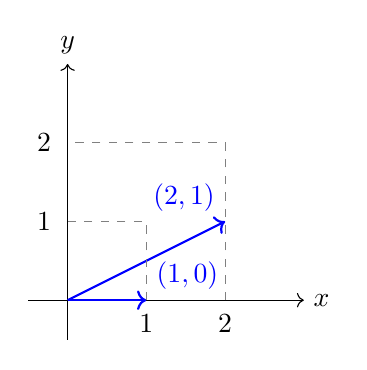
\begin{tikzpicture}
    % Draw the axes
    \draw[->] (-0.5,0) -- (3,0) node[right] {$x$};
    \draw[->] (0,-0.5) -- (0,3) node[above] {$y$};

    % Draw the vectors
    \draw[->,thick,blue] (0,0) -- (2,1) node[above left] {$(2, 1)$};
    \draw[->, thick, blue] (0,0) -- (1,0) node[above right] {$(1,0)$};
    % Draw grid lines
    \draw[dashed, gray] (1,0) -- (1,1) -- (0,1);
    \draw[dashed, gray] (2,0) -- (2,2) -- (0,2);

    % Label points
    \node at (1,-0.3) {1};
    \node at (-0.3,1) {1};
    \node at (2,-0.3) {2};
    \node at (-0.3,2) {2};
\end{tikzpicture}
\end{figure}

\[\|v_1\| = \sqrt{4+1} = \sqrt{5}\]
\[\alpha_{12} = \frac{(v_1 \mid v_2)}{(v_1 \mid v_1)} = \frac{2}{5}\]
\[u_1 = v_1\]
\[u_2 = v_2 - \alpha_{12} u_1 = \begin{pmatrix}
    1\\
    0
\end{pmatrix} - \frac{(v_1 \mid v_2)}{(v_1 \mid v_1)} \begin{pmatrix}
    1\\
    1
\end{pmatrix} = \begin{pmatrix}
    1\\
    0
\end{pmatrix} - \frac{2}{5} \begin{pmatrix}
    2\\
    1
\end{pmatrix} = \begin{pmatrix}
    \frac{1}{5}\\
    -\frac{2}{5}
\end{pmatrix}\]

\[(u_1 \mid u_2) = \begin{pmatrix}
    2 & 1
\end{pmatrix} \begin{pmatrix}
    \frac{1}{5}\\
    -\frac{2}{5}
\end{pmatrix} = \frac{2}{5} - \frac{2}{5} = 0\]
\[\left\{u_1 =  \begin{pmatrix}
    2\\
    1
\end{pmatrix}, u_2 = \begin{pmatrix}
    \frac{1}{2}\\
    -\frac{2}{5}
\end{pmatrix}\right\}\]
è una \textit{base ortogonale}.
\\
Normalizzando otteniamo:
\[u_1' = \frac{1}{\|u_1\|}\begin{pmatrix}
    2\\
    1
\end{pmatrix} = \frac{1}{\sqrt(5)} \begin{pmatrix}
    2\\
    1
\end{pmatrix} = \begin{pmatrix}
    \frac{2}{\sqrt{5}}\\
    \frac{1}{\sqrt{5}}
\end{pmatrix}\]
\[\|u_2\| = \sqrt{(u_2 \mid u_2)} = \sqrt{\frac{1}{25} + \frac{4}{25}} = \sqrt{\frac{5}{25}} = \frac{1}{\sqrt{5}}\]
\[u_2' = \frac{1}{\|u_2\|} \begin{pmatrix}
    \frac{1}{5}\\
    -\frac{2}{5}
\end{pmatrix} =  \sqrt{5} \begin{pmatrix}
    \frac{1}{5}\\
    -\frac{2}{5}
\end{pmatrix} = \begin{pmatrix}
    \frac{\sqrt{5}}{5}\\
    -\frac{2\sqrt{5}}{5}
\end{pmatrix} = \begin{pmatrix}
    \frac{1}{\sqrt{5}}\\
    -\frac{2}{\sqrt{5}}
\end{pmatrix}\]
\\
Dunque $\mathcal{B}' = \left\{\begin{pmatrix}
    \frac{2}{\sqrt{5}}\\
    \frac{1}{\sqrt{5}}
\end{pmatrix}, \begin{pmatrix}
    \frac{1}{\sqrt{5}}\\
    -\frac{2}{\sqrt{5}}
\end{pmatrix}\right\}$ è una base ortonormale di $\mathbb{R}^2$

\begin{figure}[H]
\centering
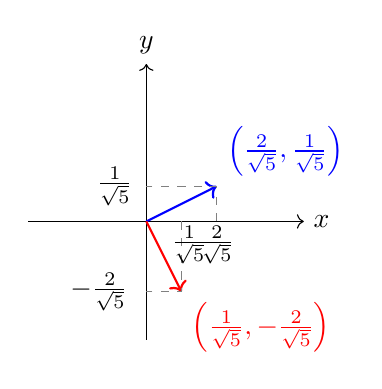
\begin{tikzpicture}
    % Define the basis vectors
    \pgfmathsetmacro{\vxA}{2/sqrt(5)}
    \pgfmathsetmacro{\vyA}{1/sqrt(5)}
    \pgfmathsetmacro{\vxB}{1/sqrt(5)}
    \pgfmathsetmacro{\vyB}{-2/sqrt(5)}

    % Draw the axes
    \draw[->] (-1.5,0) -- (2,0) node[right] {$x$};
    \draw[->] (0,-1.5) -- (0,2) node[above] {$y$};

    % Draw the vectors in the new basis
    \draw[->,thick,blue] (0,0) -- ({\vxA},{\vyA}) node[above right] {$\left(\frac{2}{\sqrt{5}},\frac{1}{\sqrt{5}}\right)$};
    \draw[->,thick,red] (0,0) -- ({\vxB},{\vyB}) node[below right] {$\left(\frac{1}{\sqrt{5}},-\frac{2}{\sqrt{5}}\right)$};

    % Draw grid lines for clarity
    \draw[dashed, gray] (\vxA,0) -- (\vxA,\vyA) -- (0,\vyA);
    \draw[dashed, gray] (\vxB,0) -- (\vxB,\vyB) -- (0,\vyB);

    % Label points
    \node at (\vxA,-0.3) {$\frac{2}{\sqrt{5}}$};
    \node at (-0.4,\vyA) {$\frac{1}{\sqrt{5}}$};
    \node at (\vxB+0.1,-0.3) {$\frac{1}{\sqrt{5}}$};
    \node at (-0.6,\vyB) {$-\frac{2}{\sqrt{5}}$};
\end{tikzpicture}
\end{figure}

\end{document}
